\documentclass[reprint,hidelinks,onecolumn]{revtex4-2}
\usepackage{braket,amsmath,color,graphicx,bookmark,bm,amssymb}
\graphicspath{{./figures/}}
\bibliographystyle{apsrev4-2}
\begin{document}

\title{\bf A Unitary RG-based Auxiliary Model Approach to Strongly-Correlated Electrons}
\author{Abhirup Mukherjee, Siddhartha Lal}
\affiliation{Department of Physical Sciences, Indian Institute of Science Education and Research-Kolkata, Mohanpur Campus, West Bengal 741246, India}
\date{\today}
\maketitle
\tableofcontents

\section{What is the minimal impurity model for a Mott metal-insulator transition?}
The Hubbard model is one of the fundamental models for strong electronic correlation; in its simplest form, it features a single band of conduction electrons hopping on a lattice and interacting via local correlations that provide a cost \(U\) if any site is doubly occupied:
\begin{equation}\begin{aligned}
	H_\text{hubb} = -t\sum_{\left<i,j \right>,\sigma}\left(c^\dagger_{i\sigma}c_{j\sigma}+\text{h.c.}\right) + U\sum_i \hat n_{i \uparrow} \hat n_{i \downarrow} - \mu \sum_{i,\sigma}\hat n_{i\sigma}~.
\end{aligned}\end{equation}
The model can be made particle-hole symmetric by choosing \(\mu = U/2\):
\[H_\text{hubb} = -t\sum_{\left<i,j \right>,\sigma}\left(c^\dagger_{i\sigma}c_{j\sigma}+\text{h.c.}\right) - \frac{U}{2}\sum_i \left(\hat n_{i \uparrow} - \hat n_{i \downarrow}\right)^2\]
There are two trivial limits of the model. At \(U=0\), the bath consists of just a kinetic energy part, and the ground state is just a filled Fermi sea. At \(t=0\), each lattice site decouples from the rest and becomes a local moment, which under symmetry-breaking becomes a Néel antiferromagnet. This suggests that on increasing \(U/t\) beyond some critical value, the system might undergo a phase transition from a metallic state to an insulating state~\cite{Mott_1949}. This transition is reflected in the local spectral function - while it has a well-defined zero energy peak in the metallic phase, it is gapped in the insulating phase.

One method of studying Hubbard models is through auxiliary models, described in the next section. Auxiliary models are simpler versions of the full Hamiltonian that are able to capture the essential physics. For example, a correlated impurity interacting with a conduction bath is a potential auxiliary model for the Hubbard Hamiltonian:
\begin{equation}\begin{aligned}
\label{clus_bath_siam}
\mathcal{H}_\text{SIAM} = \epsilon_d \hat n_d + U \hat n_{d \uparrow} \hat n_{d \downarrow} - t\sum_{\left<i,j \right>, \sigma}\left(c^\dagger_{i\sigma}c_{j\sigma} + \text{h.c.}\right) \\
+ V\sum_\sigma \left( c^\dagger_{d\sigma}c_{0\sigma} + \text{h.c.}\right) 
\end{aligned}\end{equation}
The impurity has onsite energy \(\epsilon_d\) and an onsite correlation \(U\). It hybridises into the bath through \(V\).

If the impurity site hybridises with a {\it non-interacting} bath defined by a uniform density of states, the impurity spectral function is found to have a well-defined Kondo resonance at low temperatures. Increasing the impurity correlation \(U\) only serves to reduce the width of the central peak at the cost of the appearance of side bands at energy scales of the order of \(U\), but the resonance never dies. The situation is however different if the impurity is embedded in a correlated conduction bath with a non-trivial density of states. For the case of a conduction band with the DOS shown in the right of the figure below, the impurity hybridises into a reduced bandwidth because of the correlation on the lattice~\cite{held_2013}.

This difference in the type of conduction baths is utilised in dynamical mean-field theory to describe various phases of the bulk system.
This is done through the DMFT algorithm: one starts with a non-interacting bath, but depending on the value of \(U\), the conduction bath then gets modified and we ultimately end up with something that is different from what we started with.
For small \(U\), the bath does not change much and we retain the central resonance of the impurity spectral function.
This then describes a metal in the bulk.
For larger values of \(U\), however, the bath changes significantly such that its density of states becomes non-constant.
Above a critical \(U_c\), the impurity spectral function gets gapped out, and that then describes the insulating phase in the bulk.
\textit{This leaves open the following question: What is the minimal correlation one can insert into the non-interacting bath (of a single-impurity Anderson model) that can capture both the metallic and insulating phases of the bulk model?}

\begin{figure}[!htb]
\centering
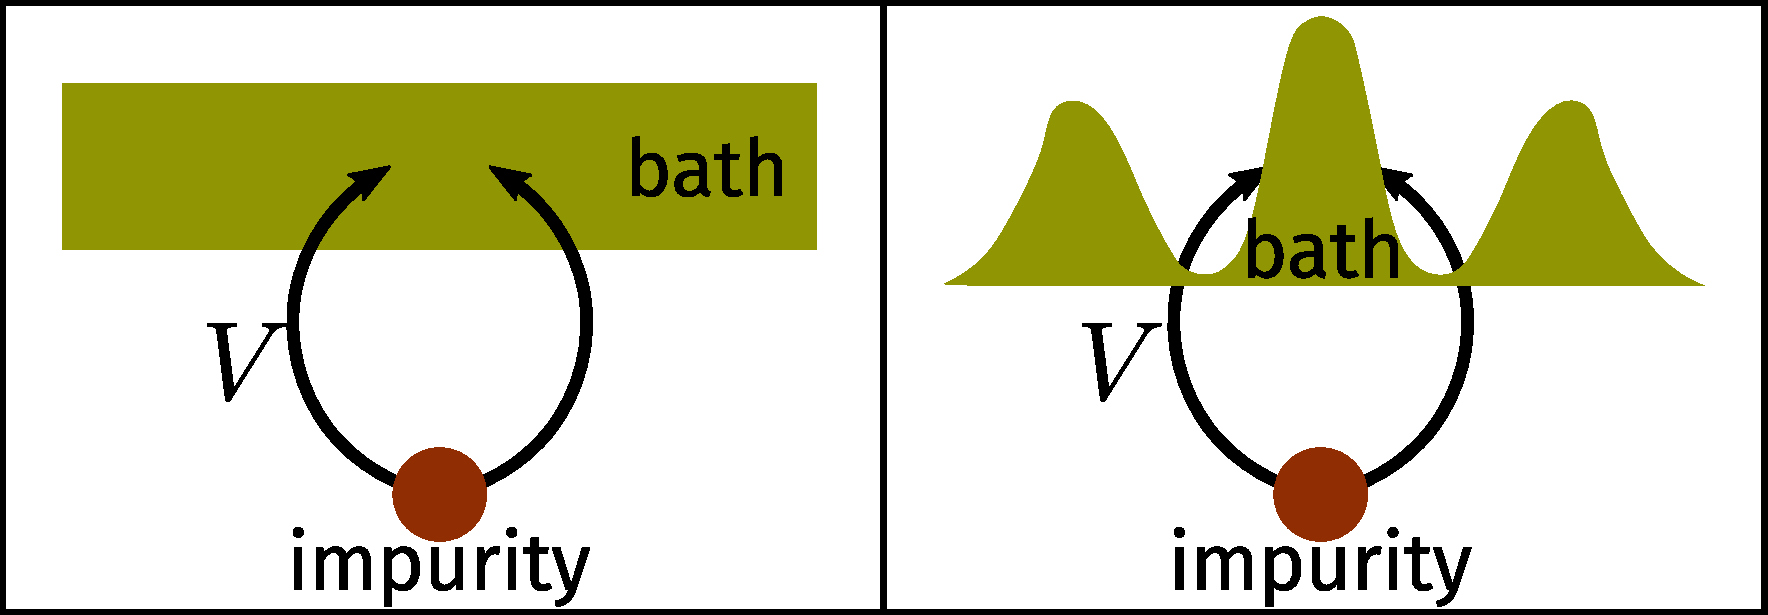
\includegraphics[width=0.45\textwidth]{dos_diff.pdf}
\caption{Various kinds of bath that an impurity can hybridise into. The left panel shows a non-interacting conduction band with a flat density of states. The right panel shows an interacting bath with an energy-dependent density of states. In the latter case, the impurity "feels" a reduced effective bandwidth defined by the width of the central peak.}
\end{figure}

\section{Philosophy of auxiliary model methods}
The present method is a realisation of the general method of using simpler systems called auxiliary models to study bulk systems~\cite{martin_2016}. In general, a full Hamiltonian can be separated into the Hamiltonians for a particular subsystem \(S\), the rest of the system \(R\), and the interactions between \(S\) and \(R\).
\begin{equation}\begin{aligned}
	\mathcal{H} &= \mathcal{H}_S\ket{S}\bra{S} + \mathcal{H}_R \ket{R}\bra{R} + \mathcal{H}_{SR} \ket{S}\bra{R} \\
				&+ \mathcal{H}_{RS}\ket{S}\bra{R} = \begin{bmatrix} & \mathcal{H}_{R} && \mathcal{H}_{RS} & \\ & \mathcal{H}_{RS}^* && \mathcal{H}_{S} & \end{bmatrix}
\end{aligned}\end{equation}
where \(\ket{S}\) and \(\ket{R}\) actually represents sums over all basis kets of \(S\) and \(R\) respectively. As an example, we can split the Hubbard model Hamiltonian between a particular site \(i = p\) and the rest of the lattice into three parts \(H_\text{hubb} = H_S + H_R + H_{SR} + H_{RS}\) (fig.~\ref{cluster-bath}), where
\begin{equation}\begin{aligned}
	H_S &= U^H\hat n_{p \uparrow} \hat n_{p \downarrow} - \mu^H \sum_\sigma \hat n_{p \sigma}\\
	H_R &= U^H\sum_{i \neq p}\hat n_{i \uparrow} \hat n_{p \downarrow} - \mu^H \sum_{i \neq p, \sigma} \hat n_{i \sigma} \\
		&-t^H\sum_{\sigma,\left<i,j \right>\atop{i \neq p \neq j}}\left(c^\dagger_{i\sigma} c_{j\sigma} + \text{h.c.}\right) \\
	H_{SR} + H_{Rs} &= - t^H\sum_{\sigma,\atop{i \in \text{N.N. of }p}}\left(c^\dagger_{i\sigma} c_{p\sigma} + \text{h.c.}\right)~.
\end{aligned}\end{equation}
The Greens function of the full Hamiltonian can also be split in a similar fashion:
\begin{equation}\begin{aligned}
	G(\omega) = \begin{bmatrix} G_S && G_{SR} \\ G_{RS} && G_R \end{bmatrix}
\end{aligned}\end{equation}
Each Greens function can be written in terms of the non-interacting counterpart and the self-energy through the Dyson equation: \(\Sigma_i = 1/G_{i,0} - 1/G_i\).

The subsystem \(S\) is usually taken to be the "cluster", and consequently, \(R\) represents the "bath".
The smaller system is typically chosen such that its eigenstates are known exactly.
Progress is then made by choosing a simpler version of \(H_R\) and a simpler form also for its coupling \(H_{RS}\) with the smaller system.
This combination of the cluster and the simpler bath is then called the \textit{auxiliary system}.
A typical auxiliary system for the Hubbard model would be the SIAM, where the impurity represents an arbitrary site \(p\) of the lattice, the bath represents the rest of the lattice sites and the hybridisation term between the impurity and the bath represents the coupling term \(H_{RS}\).
Such a construction is shown in fig.~\ref{cluster-bath}.
\begin{figure}[!htb]
	\centering
	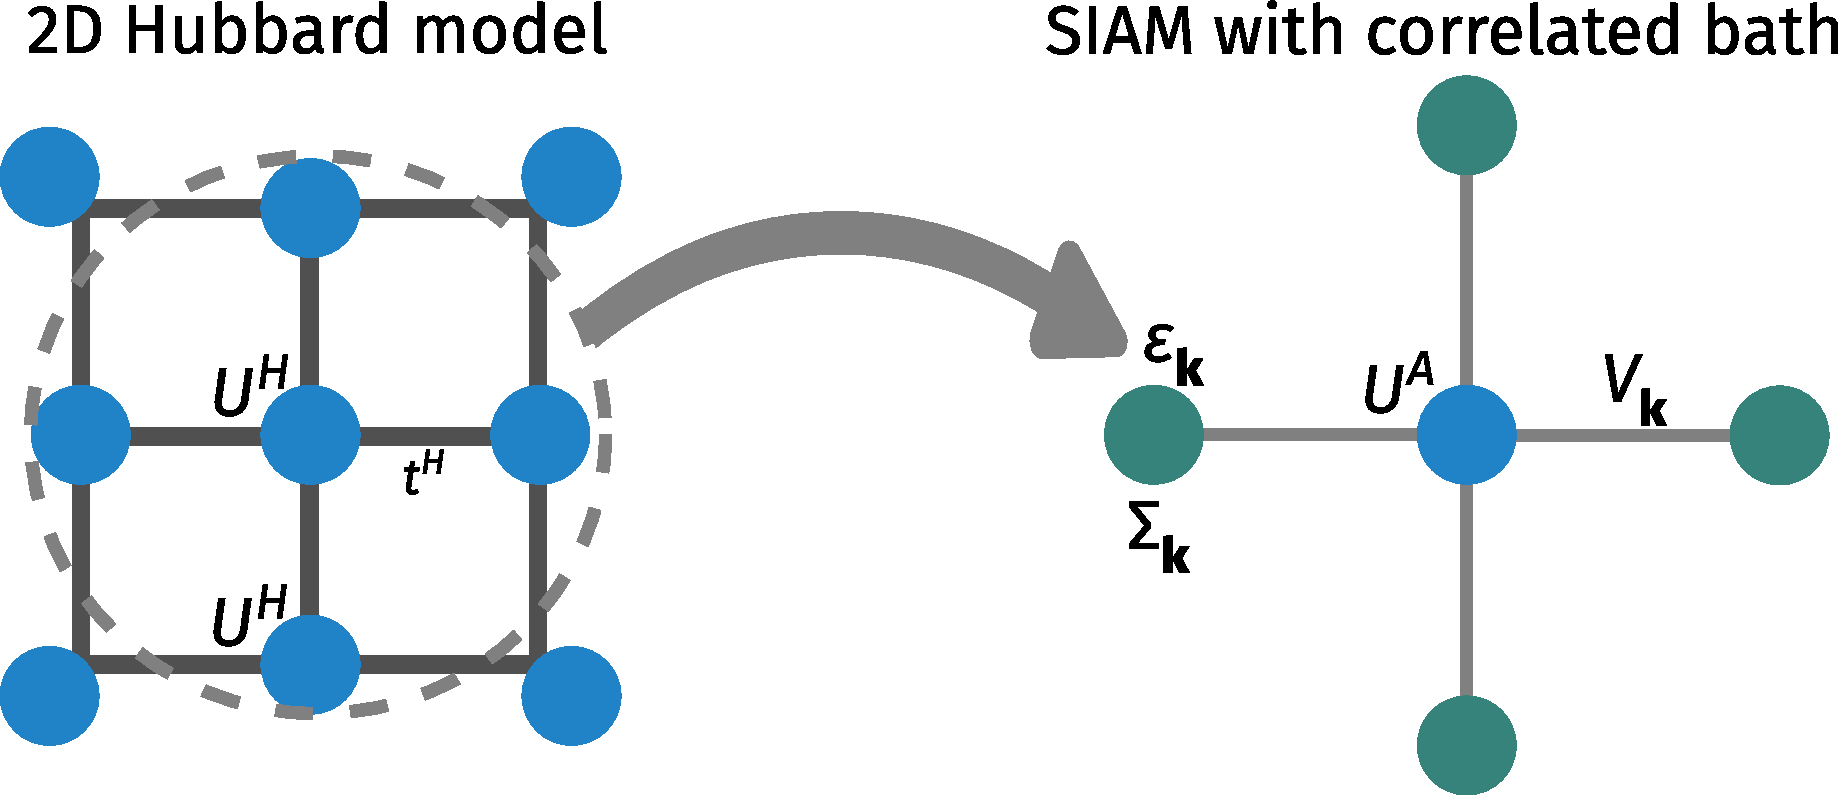
\includegraphics[width=0.48\textwidth]{clusterBath.pdf}
	\caption{\textit{Left}: Full Hubbard model lattice with onsite repulsion $U^H$ on all sites and hopping between nearest neighbour sites with strength $t^H$. \textit{Right}: Extraction of the auxiliary (cluster+bath) system from the full lattice. The central site on left becomes the impurity site (red) on the right (with an onsite repulsion $\epsilon_d$), while the rest of the $N-1$ sites on the left form a conduction bath (green circles) (with dispersion $\epsilon_k$ and correlation modelled by the self-energy $\Sigma_k(\omega)$) that hybridizes with the impurity through the coupling $V$.}
	\label{cluster-bath}
\end{figure}
\textit{It should be noted that any reasonable choice of the cluster and bath would break the translational symmetry of the full model}. To allow computing quantities, one would need to make the bath (which is a much larger system) simpler than the cluster (which is a single site). This distinction breaks the translational symmetry of the Hubbard model. For eg., if one chooses eq.~\ref{clus_bath_siam} as the auxiliary system, then the fact that the impurity has an onsite correlation while the bath does not means we have broken the symmetry between the cluster and the bath.

\subsection*{Dynamical mean-field theory - an example of an auxiliary model approach}
Dynamical mean-field theory is an approximation scheme that use impurity models to obtain Greens functions of bulk systems of strong correlation~\cite{kotliar1996,kotliar1992}. The essential idea is to find the most suitable impurity model that replicates the full Hamiltonian. This is done through the following algorithm. Given a bulk Hamiltonian with on=site correlation \(U\) and a non-interacting \(k-\)space Greens function \(G_{k,0}\) for the bath:
\begin{itemize}
	\item[1.] We first create an impurity model with on-site correlation \(U\) and non-interacting impurity Greens function \(G_{i,0} = \sum_k G_{k,0}\).
		\[\mathcal{H}_\text{aux} = H_\text{imp}(U) -t \sum_\sigma \left(c^\dagger_{d\sigma}c_{0\sigma} + \text{h.c.}\right) + H_\text{bath}\left(t,G_{i,0}\right)\]

	\item[2.] This impurity model is solved using some method like numerical renormalisation group, and the self-energy \(\Sigma_\text{aux}\) of the impurity is obtained.

	\item[3.] The impurity self-energy is now {\it equated} with the bath momentum-space self-energy:
		\[\Sigma_{k}(\omega) = \Sigma_\text{aux}(\omega)\]
		Since the impurity is purely local, this is an approximation that involves replacing a non-local quantity by its purely local component: \(\Sigma_{k}(\omega) = \sum_{{\bf r}}e^{i \vec{k}\cdot\vec{r}}\Sigma_{{\bf r}}(\omega) \simeq \Sigma_{{\bf r} = 0}(\omega)\). This approximation is a result of the single-site nature of the cluster of the chosen auxiliary model - larger clusters with more impurities can generate non-local components. This local approximation becomes exact in the limit of large system dimension \(w\), because it can be shown that the non-local components of the self-energy scale as \(w^{-3/2}\).

	\item[4.] With this updated bath self-energy, we now create a new \(k-\)space Greens function for the bath:
		\begin{equation}\begin{aligned}
		G_{i}(\omega) &= \sum_k G_{k}(\omega) \\
			      &= \sum_k \frac{1}{\omega - H_\text{bath}(k) - \Sigma_k(\omega)} \\
			      &= \sum_k \frac{1}{\omega - H_\text{bath}(k) - \Sigma_\text{aux}(\omega)}
		\end{aligned}\end{equation}
	This interacting Greens function is then used to obtain the updated non-interacting Greens function, using Dyson's equation:
	\[G_{i,0} = \frac{1}{1/G_{i} + \Sigma_\text{aux}}\]
	\item[5.] Repeat the algorithm from step 1 with the updated \(G_{i,0}\), until \(\Sigma_\text{aux}\) stops changing.
\end{itemize}
The stopping condition is the consistency relation that makes the bath and impurity self-energies equal.

\begin{figure}[!htb]
	\centering
	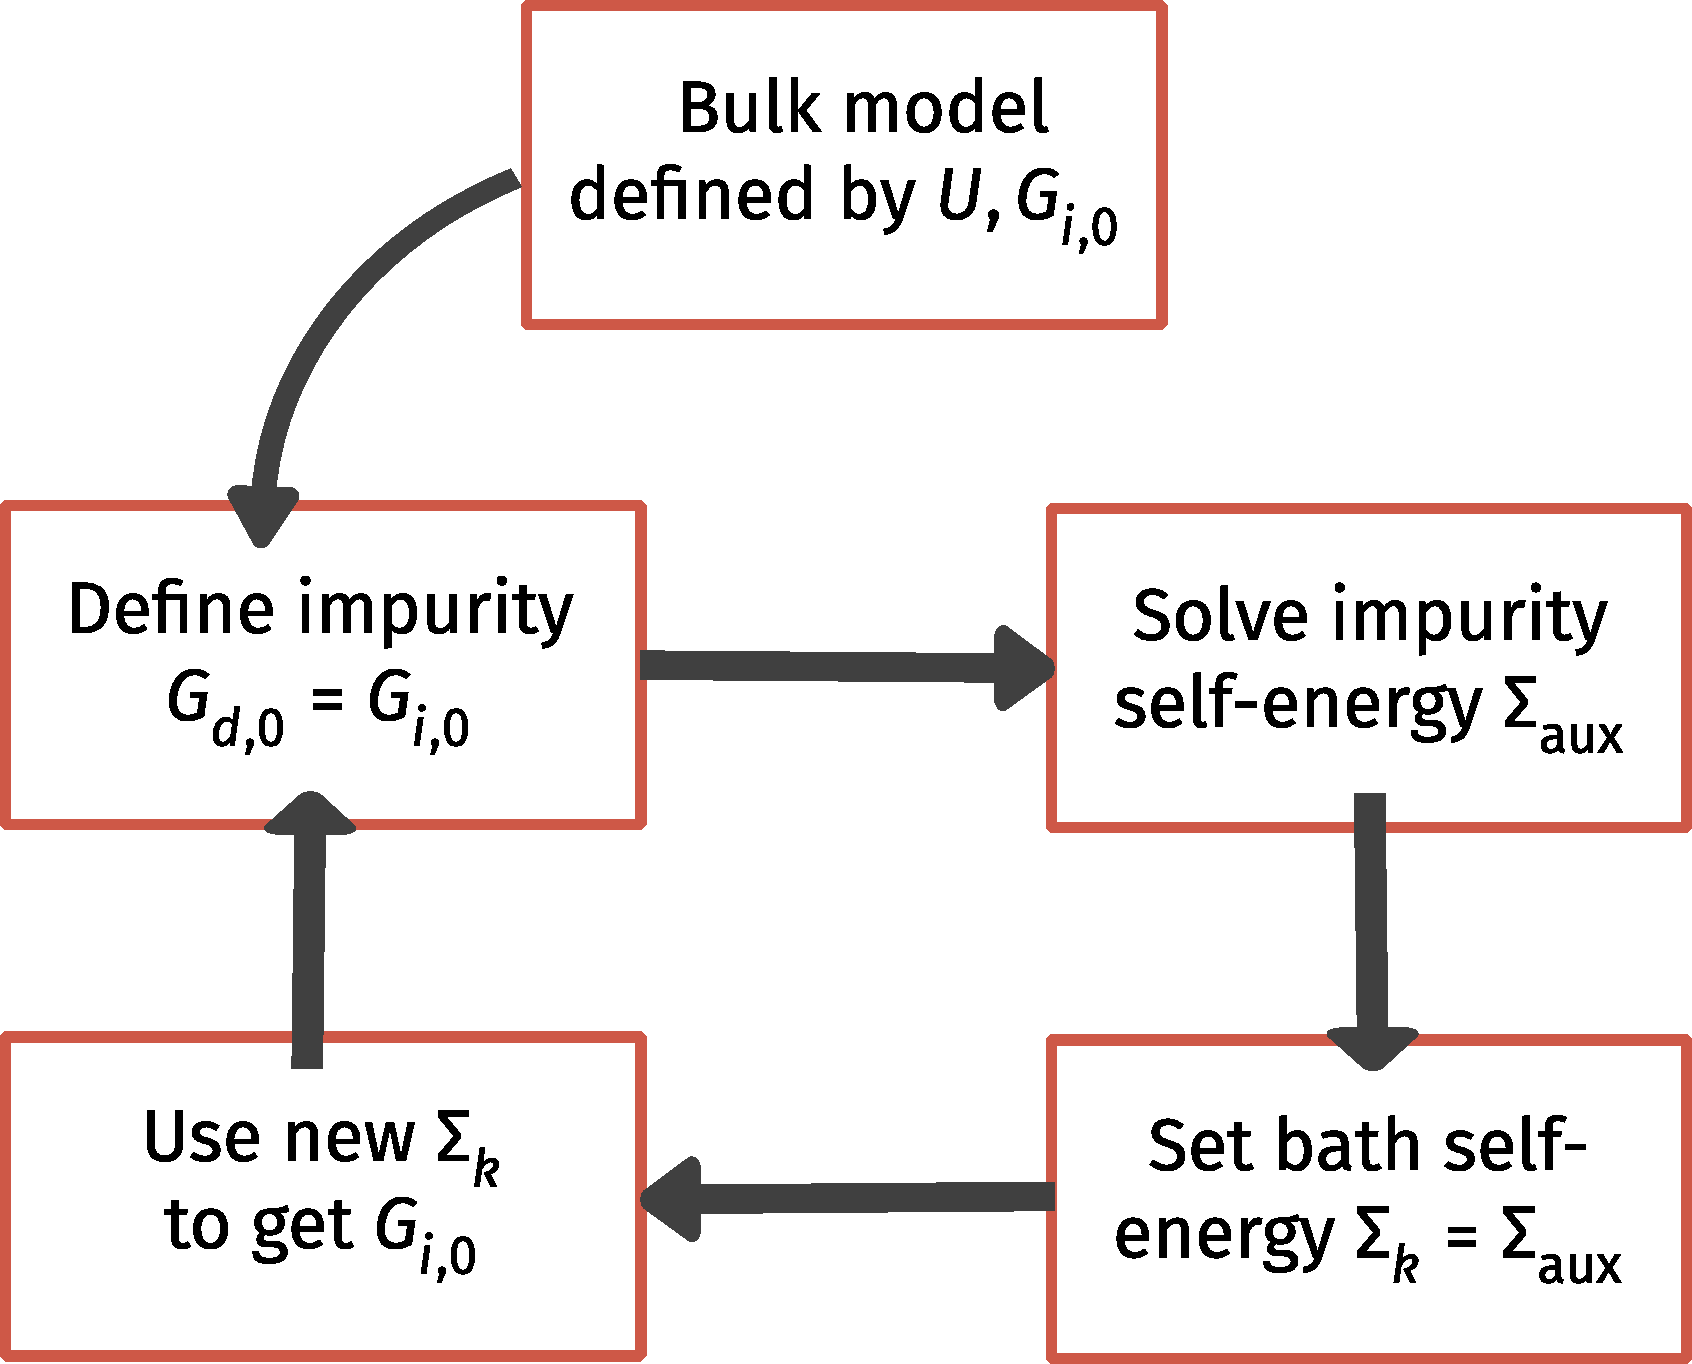
\includegraphics[width=0.35\textwidth]{dmft_scheme.pdf}
\end{figure}


\section{A ``bottoms-up" approach to using auxiliary models}
As mentioned in the previous section, the question we are posing is the following: what is the simplest auxiliary model of impurity in a bath that can capture the metal-insulator transition in a Hubbard-like model of correlated electrons. We approach this problem in a constructionist/bottoms-up way: we first identity an appropriate quantum impurity model (fig.~\ref{cluster-bath}) that shows an impurity phase transition, and then create a bulk model out of this auxiliary model. The bulk model hence created will then show a metal-insulator transition. 

The impurity models are studied using the recently-developed unitary renormalisation group method~\cite{anirbanmott1,anirbanmott2,anirbanurg1,anirbanurg2,siddharthacpi,santanukagome}. The leap to the bulk model is then made by applying lattice translation operators on the auxiliary model. This process, referred to as tiling here, relates the auxiliary model Hamiltonian with that of the bulk, and hence allows connecting the Greens functions and other related quantities across dimensions. One nice outcome is that since the auxiliary model has multiple sites, there is a real-space off-diagonal component of the self-energy, and this leads to a \(k-\)dependence in the self-energy of the bulk, which is in contrast with the lack of \(k-\)dependence in single-site DMFT.  

In our approach, the auxiliary models can be chosen in various ways. The simplest choice is of course the single-impurity Anderson model of eq.~\ref{clus_bath_siam}:
\begin{equation}\begin{aligned}
\mathcal{H}_\text{SIAM} = \epsilon_d \hat n_d + U \hat n_{d \uparrow} \hat n_{d \downarrow} - t\sum_{\left<i,j \right>, \sigma}\left(c^\dagger_{i\sigma}c_{j\sigma} + \text{h.c.}\right) \\
+ V\sum_\sigma \left( c^\dagger_{d\sigma}c_{0\sigma} + \text{h.c.}\right) 
\end{aligned}\end{equation}
This model does not show any impurity phase transition - the impurity is always screened~\cite{hrk_wilson_1980,wilson1975,bullaNRGreview}. Correlation can be introduced into the auxiliary model in two ways:
\begin{itemize}
	\item[1.] The impurity or the bath can be made to have additional interaction: 
\begin{gather}
\mathcal{H}_\text{aux} = H_\text{SIAM} + J \vec{S}_d\cdot\vec{s}_0 - \frac{1}{2}U_b \left(\hat n_{0 \uparrow} - \hat n_{0 \downarrow}\right)^2
\end{gather}
The additional terms are (i) a spin-exchange interaction between the impurity site and the zeroth site, and (ii) a local correlation on the zeroth site.
\item[2.] The second method is to make the cluster itself more complicated. That is, one can introduce multiple impurity sites that are connected via the hopping:
	\begin{equation}\begin{aligned}
	\mathcal{H}_\text{aux} = -\frac{U}{2}\sum_{d_i}\left(\hat n_{d_i \uparrow} - \hat n_{d_i \downarrow}\right) ^2 + V\sum_{d_i}\sum_\sigma\left( c^\dagger_{d_i\sigma}c_{0\sigma} + \text{h.c.} \right) \\
	+ \text{K.E.} - t\sum_{\sigma}\left(c^\dagger_{d_1\sigma}c_{d_2\sigma} + \text{h.c.}\right)
	\end{aligned}\end{equation}
	
\end{itemize}

\begin{figure}[!htb]
 	\centering
 	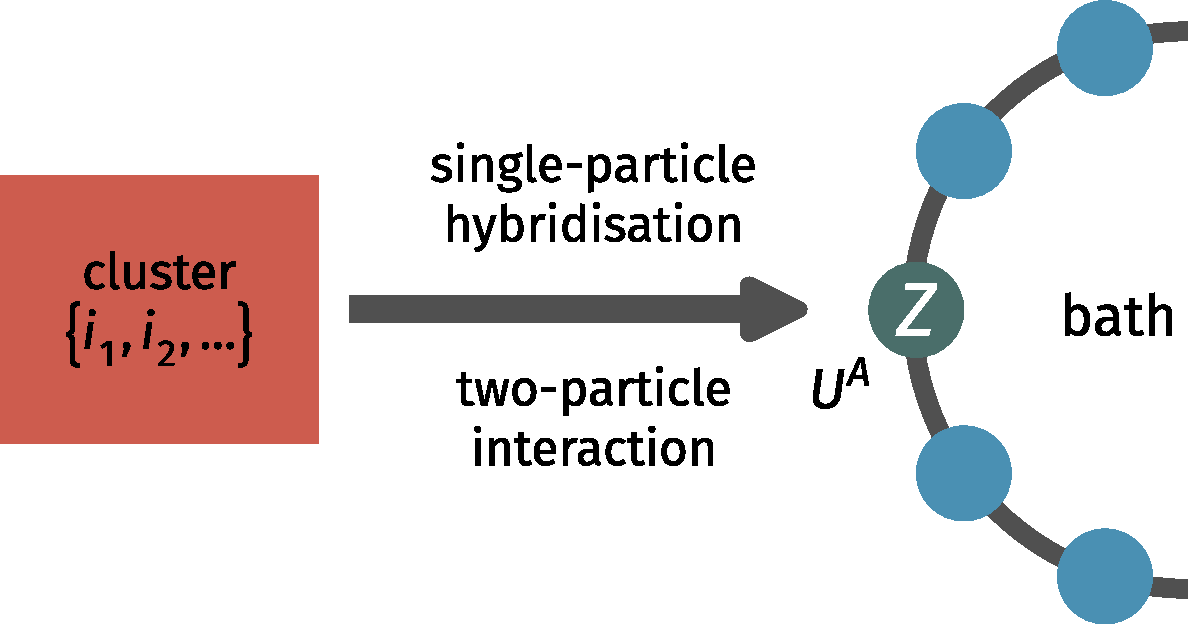
\includegraphics[width=0.35\textwidth]{gen_siam.pdf}
 	\caption{Cluster+bath construction of auxiliary model. It consists of a cluster (red square) hybridising with a bath (ring) by hopping into and out of the zeroth site (pink). The other sites (green) form the rest of the bath. Just the cluster and the zeroth site have onsite correlations.}
 \end{figure}
 The next step in the programme is to tile the real-space lattice with this cluster+bath Hamiltonian \(\tilde H\) to restore translational invariance (shown in a later section), and obtain a new bulk Hamiltonian for correlated electrons, $\tilde H = T\left[ \mathcal{H}_\text{aux} \right] T^{-1}$, where $T$ denotes the operator that performs the set of iterative real-space translations, and enables the cluster-bath (auxiliary model) Hamiltonian to span the target real-space lattice. Given a general auxiliary model Hamiltonian \(\mathcal{H}_\text{aux}\), the result of tiling can be written very generally as
 \begin{equation}\begin{aligned}
	 \tilde H = \sum_{\left\{i_1,i_2,...\right\}} \mathcal{H}_\text{aux}\left(\left\{i_1,i_2,...\right\}\right)
 \end{aligned}\end{equation}
where \(\left\{i_1,i_2,...\right\}\) represents the indices for the members of the cluster. To reiterate, what that means is that we have placed the cluster+bath system at all lattice point sets \(\left\{i_1,i_2,...\right\}\) to reconstruct a new model of correlated electrons. The answer to how closely $\tilde H$ approximates a target model of correlated electrons lies in (i) the choice of the cluster-bath construction of the auxiliary model, and (ii) the accuracy of the URG procedure on the auxiliary model.

The strategy, therefore, is to relate Hamiltonians, wavefunctions and hence correlation functions of the bulk model to those of the auxiliary model. One can then substitute the information obtained from solutions of the auxiliary model, and thereby calculate quantities on the bulk lattice model.

\section{Extending the Anderson impurity model}
We have shown in a previous work that by including a local attractive interacting on the conduction bath site coupled to the impurity site of the Anderson impurity model, one can obtain an impurity phase transition from a screened phase to an unscreened local moment phase at a certain critical value of the attractive interaction strength. We now consider a more realistic form of this model, by embedding the impurity site into the lattice of a 2D  conduction bath and accounting for the lowering of the \(s-\)wave symmetry of the interactions down to just the \(C_4\) symmetry of the 2D square lattice. A general structure of such a model is shown in fig.~\ref{embeddedEsiam}; one of the sites of the 2D square lattice is identified as the impurity, while the four nearest-neghbours interact directly with this impurity site. 
\begin{figure}[htpb]
	\centering
	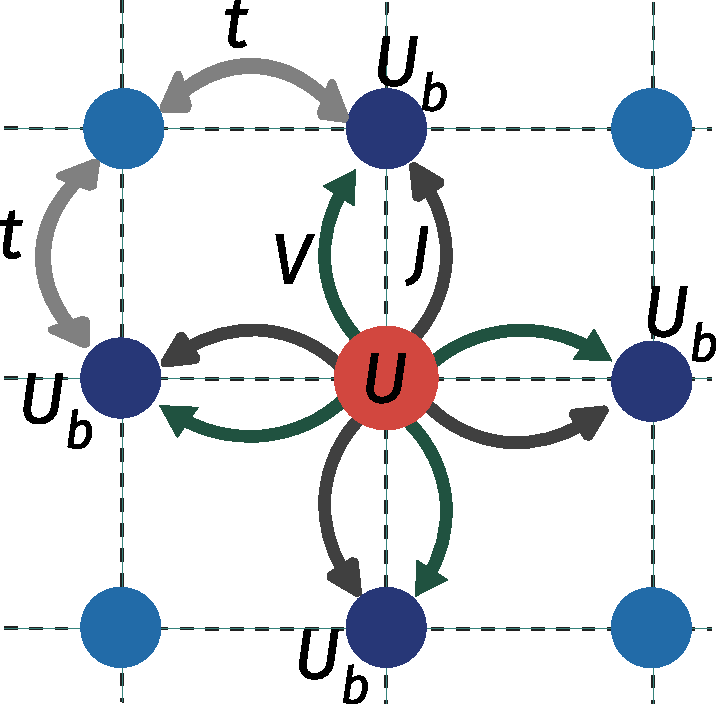
\includegraphics[width=0.2\textwidth]{pWaveEsiam.pdf}
	\caption{General structure of an embedded extended SIAM, where the impurity site is a part of the 2D square lattice. The four nearest-neghbour sites (dark blue) interact with the impurity site through one or more processes, and can host local interactions. The other lattice sites (light blue) are completely non-interacting.}
	\label{embeddedEsiam}
\end{figure}
\subsection{Hamiltonian}
We consider an impurity spin \(\vec S_d\) interacting with a two-dimensional tight-binding conduction bath through a highly localised interaction, described by the Hamiltonian
\begin{equation}\begin{aligned}
	\mathcal{H} = H_\text{cbath} + H_\text{imp-cbath} + H_\text{cbath-int}~,
\end{aligned}\end{equation}
where \(H_\text{cbath}\) is the kinetic energy arising out of nearest-neighbour hopping processes,
\begin{equation}\begin{aligned}
	H_\text{cbath} = -2t\sum_{{\bf k}}\left[\cos(ak_x) + \cos(ak_y)\right] c^\dagger_{{\bf k},\sigma}c_{{\bf k},\sigma}~.
\end{aligned}\end{equation}
The form of the impurity-bath interaction \(H_\text{imp-cbath}\) and the local interaction \(H_\text{cbath-int}\) in the bath can be of various forms, depending in the choice of the bath orbital which participates in the interaction. We now consider some interesting cases:
\paragraph{\(d-\)wave interactions:} This is the case when a coherent \(d-\)wave combination of the bath sites closest to the impurity participates in the interaction:
\begin{equation}\begin{aligned}
	d_{\sigma} &= \frac{1}{2}\left(c^\dagger_{L,\sigma} + c^\dagger_{R,\sigma} - c^\dagger_{U\sigma} - c^\dagger_{D\sigma}\right)~,
\end{aligned}\end{equation}
leading to the interaction terms
\begin{equation}\begin{aligned}
	H^{(d)}_\text{imp-cbath} &= J\vec{S}_d\cdot\frac{1}{2}\sum_{\sigma_1,\sigma_2}\vec{\tau}_{\sigma_1,\sigma_2} d^\dagger_{\sigma_1}d_{\sigma_2}~,\\
	H^{(d)}_\text{cbath-int} &= -\frac{W}{2}\left(d^\dagger_{\uparrow}d_{\uparrow} - d^\dagger_{\downarrow}d_{\downarrow}\right)^2~,
\end{aligned}\end{equation}
where \(\vec \tau\) is the vector of sigma matrices, \(\sigma_1,\sigma_2\) are spin indices, and \(L,R,U,D\) represent the four lattice sites ({\it L}eft, {\it R}ight, {\it U}p, {\it D}own) closest to the impurity. When Fourier-transformed to momentum space, it gives rise to the momentum-dependent couplings
\begin{equation}\begin{aligned}\label{d-wave k-space}
	J_{{\bf k}_1, {\bf k}_2} = J f_{\pi}\left({\bf k}_1\right) f_{\pi}\left({\bf k}_2\right) ~,\quad W_{\left\{ k_i \right\} } = W\prod_{i=1,2,3,4}f_{\pi}(k_i)~,
\end{aligned}\end{equation}
where \(f_{\pi}({\bf k}) = \cos\left( ak_x \right) - \cos\left( ak_y \right) \) is the \(d-\)wave symmetric functional form in \(k-\)space.
\paragraph{\(p-\)wave interaction:} One can also consider the case when the \(p-\)wave orbital of the nearest sites participates in the interaction:
\begin{equation}\begin{aligned}
	p_{\sigma} &= \frac{1}{2}\left(c^\dagger_{L,\sigma} + c^\dagger_{R,\sigma} + c^\dagger_{U\sigma} + c^\dagger_{D\sigma}\right)~,\\
	H^{(p)}_\text{imp-cbath} &= J\vec{S}_d\cdot\frac{1}{2}\sum_{\sigma_1,\sigma_2}\vec{\tau}_{\sigma_1,\sigma_2} p^\dagger_{\sigma_1}p_{\sigma_2}~,\\
	H^{(p)}_\text{cbath-int} &= -\frac{W}{2}\left(p^\dagger_{\uparrow}p_{\uparrow} - p^\dagger_{\downarrow}p_{\downarrow}\right)^2~.
\end{aligned}\end{equation}
The momentum-dependent Kondo coupling in this case is 
\begin{equation}\begin{aligned}\label{p-wave k-space}
	J_{{\bf k}_1, {\bf k}_2} = J f_{{2\pi}}\left({\bf k}_1\right) f_{{2\pi}}\left({\bf k}_2\right) ~, \quad W_{\left\{ k_i \right\} } = W\prod_{i=1,2,3,4}f_{{2\pi}}(k_i)~,
\end{aligned}\end{equation}
where \(f_{2\pi}({\bf k}) = \cos\left( ak_x \right) + \cos\left( ak_y \right)\) is the form for the \(p-\)wave symmetric function.

Note that both these interactions involve not only local terms as well as quasi-local terms in the form of off-site interactions that connect the impurity site with multiple bath sites. An example of such a term is \(\vec{S}_d\cdot\frac{1}{2}\sum_{\sigma_1,\sigma_2}\vec{\tau}_{\sigma_1,\sigma_2} c^\dagger_{R,\sigma_1}c_{U,\sigma_2}\), which couples the impurity site with both the right and up sites in the bath. One can consider simple modifications of these cases by retaining only the on-site terms in the interaction Hamiltonian. This gives us the modified \(d-\)wave and \(p-\)wave symmetries:
\begin{equation}\begin{aligned}
	H^{(\bar d(\bar p))}_\text{imp-cbath} &= J\vec{S}_d\cdot\frac{1}{2}\sum_{\sigma_1,\sigma_2}\vec{\tau}_{\sigma_1,\sigma_2} \sum_{i \in \left\{L,R,U,D\right\}} \lambda_i c^\dagger_{i,\sigma_1}c_{i,\sigma_2}~,\\
	H^{(\bar d(\bar p))}_\text{cbath-int} &= -\frac{W}{2}\sum_{i \in \left\{L,R,U,D\right\}} \lambda_i \left(c^\dagger_{i, \uparrow}c_{i, \uparrow} - c^\dagger_{i, \downarrow}c_{i, \downarrow}\right) ~,
\end{aligned}\end{equation}
where \(\lambda_R = \lambda_L = \lambda_U = \lambda_D = 1\) for the \(\bar p\)-wave case, but \(\lambda_R = \lambda_L = -\lambda_U = -\lambda_D = 1\) for the \(\bar d\)-wave case. The \(k-\)dependent couplings have the form
\begin{equation}\begin{aligned}
	J_{{\bf k}_1, {\bf k}_2} &= J f_{\bar d(\bar p)}\left({\bf k}_1 -{\bf k}_2\right),\\
	W_{\left\{ \bf k_i \right\} } &= Wf_{\bar d(\bar p)}\left({\bf k}_1 -{\bf k}_2 + {\bf k}_3 -{\bf k}_4\right) ,
\end{aligned}\end{equation}
where 
\begin{equation}\begin{aligned}
	&f_{\bar d(\bar p)}\left({\bf k}_1 -{\bf k}_2 + {\bf k}_3 -{\bf k}_4\right) \\
	&= \frac{1}{2}\left[\lambda_R \cos\left(k_{1x} - k_{2x} + k_{3x} - k_{4x}\right) \right.\\
	&\quad\left. + \lambda_U \cos\left(k_{1y} - k_{2y} + k_{3y} - k_{4y}\right)\right] ~.
\end{aligned}\end{equation}

\subsection{Unitary RG analysis of the model}
We studied the low-energy physics of this model through a unitary renormalisation group calculation that decouples the high-energy modes of the conduction bath and incorporates their effects in the form of renormalised Hamiltonian couplings. We find that the bath interaction \(W\) remains marginal (does not undergo any renormalisation), while the renormalisation in the momentum-resolved Kondo coupling \(J^{(j)}\) at the \(j^\text{th}\) step is of the form
\begin{equation}\begin{aligned}\label{KondoRGequation}
	\Delta J^{(j)}_{{\bf k}_1, {\bf k}_2} = -\sum_{{\bf q} \in \text{PS}} \frac{J^{(j)}_{{\bf k}_2,{\bf q}} J^{(j)}_{{\bf q},{\bf k}_1} + 4J^{(j)}_{{\bf q}, {\bf \bar q}} W_{{\bf \bar q}, {\bf k}_2, {\bf k}_1, {\bf q}}}{\omega - \frac{1}{2}|\varepsilon_j| + J^{(j)}_{{\bf q}}/4 + W_{{\bf q}}/2}~,
\end{aligned}\end{equation}
where \(\varepsilon_j\) is the energy of the shell being decoupled at the \(j^\text{th}\) step, and the sum is over all momentum states \({\bf q}\) in the particle sector (PS) of the shell \(\varepsilon_j\) (that is, all states that are occupied at \(T=0\) and in the absence of any quantum fluctuations). The Kondo coupling and the RG equation as well have certain symmetries under transformations in the Brillouin zone. If any one of the momenta \({\bf k}_1\) or \({\bf k}_2\) are translated by \(\pi\) (\(k_{1x} \to k_{1x} + \pi, k_{1y} \to k_{1y}+\pi\)), the coupling as well as the RG equation changes sign. Translating both the momenta leads to the reversal of the sign change. 
\begin{equation}\begin{aligned}\label{hamiltonanSymms}
	\Delta J^{(j)}_{{\bf k}_1 + \boldsymbol{\pi}, {\bf k}_2} = \Delta J^{(j)}_{{\bf k}_1, {\bf k}_2 + \boldsymbol{\pi}} = -\Delta J^{(j)}_{{\bf k}_1 + \boldsymbol{\pi}, {\bf k}_2 + \boldsymbol{\pi}} = -\Delta J^{(j)}_{{\bf k}_1, {\bf k}_2}~.
\end{aligned}\end{equation}
These transformations involve translating one or both momenta through the center of the Brillouin zone.

We now consider some specific cases of these results.
\paragraph{Interactions with off-site terms:}
The case with the complete \(d-\)wave and \(p-\)wave terms enjoy a factorisation of the momentum space couplings into functions of the participating momenta, as shown in eq.~\ref{d-wave k-space} and \ref{p-wave k-space}. This factorisation also translates into the RG equation, ensuring that the momentum space Kondo coupling retains its form, and renormalisation occurs only in the magnitude \(J\), through the equation
\begin{equation}\begin{aligned}
	\Delta J^{(j)}_{{\bf k}_1, {\bf k}_2} &= f_{{2\pi}(\pi)}\left({\bf k}_1\right) f_{{2\pi}(\pi)}\left({\bf k}_2\right) \Delta J~,\\
\Delta J &= \sum_{{\bf q} \in \text{PS}} \frac{-f_{2\pi(\pi)}({\bf q})^2\left[J^2 + 4JWf_{2\pi(\pi)}({\bf q})^2\right]}{\omega - \frac{1}{2}|\varepsilon_j| + \frac{J}{4}f_{2\pi(\pi)}({\bf q})^2 + \frac{W}{2}f_{2\pi(\pi)}({\bf q})^4}~.
\end{aligned}\end{equation}
\paragraph{Interactions without off-site terms:}
This choice does not lead to a factorisation of the momentum-space dependence, and the form of the Kondo coupling therefore morphs during the RG flow, allowing the emergence of new degrees of freedom that screen the impurity at low-energies. At the first step, the RG equation can be written down explicitly as
\begin{equation}\begin{aligned}
	&\Delta J^{(0)}_{{\bf k}_1, {\bf k}_2} =\\
	&-\sum_{{\bf q} \in \text{PS}} \frac{J^2 f_{\bar p(\bar d)}\left({\bf k}_2 - {\bf q}\right) f_{\bar p(\bar d)}\left({\bf q} - {\bf k}_1\right) - 4JW f_{\bar p(\bar d)}\left({\bf k}_2 - {\bf k}_1\right)}{\omega - \frac{1}{2}|\varepsilon_j| + \frac{J}{4}f_\mathcal{D}({\bf q})^2 + \frac{W}{4}}
\end{aligned}\end{equation}
The first term in the numerator does not depend only on the momentum difference \({\bf k}_2 - {\bf k}_1\), unlike the bare Kondo coupling. This leads to a new \(k-\)space dependence of the Kondo coupling at the second step, hence leading to a modified RG equation if one makes the \(k-\)dependence explicit.

\section{The Tiling Algorithm}

\subsection{Formal description of the tiling procedure}
We will now define the {\it tiling} procedure by which we can recreate the complete lattice model by using instances of an auxiliary model Hamiltonian. The first step is of course to identify an impurity model that can act as a good auxiliary model for out lattice model. The local behaviour of this impurity model should reflect the essential local physics of the lattice model. Typically, we will consider impurity model geometries where the real-space bath site connected directly to the impurity also harbours some kind of local interaction. We will henceforth refer to this site as the zeroth site. In the case where multiple sites are connected directly to the impurity, we will choose one of these sites for reference and call that the {\it bath zeroth site} throughout.

In order to identify a {\it unit cell} for our tiling procedure, we place the impurity site at a reference site \({\bf r}_d\) of our lattice, and the bath zeroth site at a nearest-neighbour site \({\bf z}\), and label the corresponding auxiliary model Hamiltonian as \(\mathcal{H}_\text{aux}({\bf r}_d, {\bf z})\). The unit cell at the position \({\bf r}_d\) is then obtained by placing the zeroth site on all nearest-neighbours of \({\bf r}_d\) and averaging over these configurations:
\begin{equation}\begin{aligned}\label{unitCellHamiltonian}
	\mathcal{H}_\text{aux}({\bf r}_d) = \frac{1}{\mathcal{Z}}\sum_{{\bf z}\in\text{NN}({\bf r}_d)}\mathcal{H}_\text{aux}({\bf r}_d, {\bf z})~,
\end{aligned}\end{equation}
where \({\bf z}\) is summed over all nearest-neighbours of \({\bf r}_d\) and \(\mathcal{Z}\) is the number of such nearest-neighbours.

In order to create the bulk model, we now need to translate this auxiliary model over the entire lattice. For this, we define {\it many-particle global} translation operators \(T({\bf a})\) that translate all positions by a vector \({\bf a}\). In terms of manybody states and operators, their action is defined as 
\begin{equation}\begin{aligned}\label{translationDefinition}
	&T^\dagger({\bf a}) \ket{{\bf r}_1, {\bf r}_2,\ldots} = \ket{{\bf r}_1 + {\bf a}}\otimes\ket{{\bf r}_2 + {\bf a}}\ldots\otimes\ket{{\bf r}_n + {\bf a}}\\
	&T^\dagger({\bf a}) \mathcal{O}\left({\bf r}_1, {\bf r}_2,\ldots\right)T({\bf a}) = \mathcal{O}\left({\bf r}_1 + {\bf a}, {\bf r}_2 + {\bf a},\ldots\right)~,
\end{aligned}\end{equation}
where \(\ket{{\bf r}_1, {\bf r}_2,\ldots}\) is a state in the manyparticle Fock-space basis with the particles localised at the specified positions. For example, for a local fermionic creation operator \(c^\dagger({\bf r})\), we have 
\begin{equation}\begin{aligned}
	T^\dagger({\bf a}) c^\dagger({\bf r}) T({\bf a}) = c^\dagger({\bf r} + {\bf a})~.
\end{aligned}\end{equation}
It acts similarly on the auxiliary model Hamiltonian:
\begin{equation}\begin{aligned}
	T^\dagger({\bf a})\mathcal{H}_\text{aux}({\bf r}_d)T({\bf a}) = \mathcal{H}_\text{aux}({\bf r}_d + {\bf a})~,
\end{aligned}\end{equation}
translating all sites by the vector \({\bf a}\). By introducing the Fourier transform to momentum space,
\begin{equation}\begin{aligned}
	\ket{{\bf r}_1, {\bf r}_2,\ldots} = \otimes_{j=1}^N \int d{\bf k}_j e^{-i {\bf r}_j\cdot{\bf k}_j} \ket{{\bf k}_j}~,
\end{aligned}\end{equation}
it is easy to see that the total momentum states are eigenstates of the global translation operators:
\begin{equation}\begin{aligned}
	T^\dagger({\bf a})\ket{{\bf k}_1, {\bf k}_2,\ldots} &= \otimes_{j=1}^N \int d{\bf r}_j e^{i {\bf r}_j\cdot{\bf k}_j} T^\dagger({\bf a})\ket{{\bf r}_j}~,\\
							    &=\otimes_{j=1}^N \int d{\bf r}_j e^{i {\bf r}_j\cdot{\bf k}_j} \ket{{\bf r}_j + {\bf a}}\\
							    &=e^{-i {\bf a}_j\cdot{\bf k}_\text{tot}}\ket{{\bf k}_1, {\bf k}_2,\ldots},
\end{aligned}\end{equation}
where \({\bf k}_\text{tot} = \sum_j {\bf k}_j\) is the total momentum.

The auxiliary model, being an impurity model, lacks translation symmetry. The lattice model does remain invariant under global translation operations. In order to reconstruct the full lattice model and restore its translation invariance, we translate the unit cell across all sites of the lattice:
\begin{equation}\begin{aligned}
	\label{tilingPrescription}
	\mathcal{H}_\text{tiled} &= \sum_{{\bf r}}\mathcal{H}_\text{aux}({\bf r})\\
				&= \sum_{{\bf r}}T^\dagger({\bf r} - {\bf r}_d)\mathcal{H}_\text{aux}({\bf r}_d)T({\bf r} - {\bf r}_d)~ \\
				&= \frac{1}{\mathcal{Z}}\sum_{{\bf r}}\sum_{{\bf z}\in\text{NN}({\bf r}_d)}T^\dagger({\bf r} - {\bf r}_d)\mathcal{H}_\text{aux}({\bf r}_d, {\bf z})T({\bf r} - {\bf r}_d)~ \\
\end{aligned}\end{equation}
where \({\bf r}\) sums over all lattice sites.

\subsection{Extending the Anderson impurity model: Identifying the correct auxiliary model}
The standard Anderson model consists of a correlated impurity site coupled with a non-interacting conduction bath. The double occupancy cost on the impurity is \(U\), while the single-particle hopping strength between the impurity and the conduction bath is \(V\). Such a model does not exhibit a phase transition; the low-energy phase is one of strong-coupling for all parameter regimes. We have recently studied an extended Anderson impurity model (e-SIAM) where we introduced an explicit Kondo coupling \(J\) and a local correlation \(U_b\) on the bath zeroth site, which is the site connected to the impurity (see \cite{gazizovaleblanc2023} for some recent findings of non-local effective attractive interactions within the Hubbard model). The Hamiltonian of the e-SIAM for a half-filled impurity site is of the form
\begin{equation}\begin{aligned}
	\label{siam_attr}
	\mathcal{H}_\text{E-S} = \mathcal{H}_\text{cbath} + \mathcal{H}_\text{imp} + \mathcal{H}_\text{imp-cbath}~,
\end{aligned}\end{equation}
where 
\begin{itemize}
	\item \(\mathcal{H}_\text{cbath} = -\frac{1}{\mathcal{Z}}t\sum_{i=0,1,\ldots;\sigma}\left(c^\dagger_{i,\sigma}c_{i+1,\sigma} + \text{h.c.}\right) - \frac{1}{2}U_b\left(\hat n_{0 \uparrow} - \hat n_{0 \downarrow}\right)^2\) is the Hamiltonian of the conduction bath consisting of a kinetic energy term and some local interaction terms on the zeroth site,
	\item \(\mathcal{H}_\text{imp} = - \frac{U}{2}\left(\hat n_{d \uparrow} - \hat n_{d \downarrow} \right) ^2\) is the Hamiltonian for the localised impurity site, and
	\item \(\mathcal{H}_\text{imp-bath} = J {\bf S}_d\cdot{\bf S}_0 - V \sum_{\sigma} \left(c^\dagger_{0\sigma} c_{d\sigma} + h.c.\right)\) describes the interaction between the impurity orbitals and the conduction bath.
\end{itemize}
Here, \(c_{d\sigma}\) is the impurity electron operator, \(c_{i\sigma}\) is the conduction bath electron operator, \(c_{0,\sigma}\) is the bath zeroth site operator, \({\bf S}_d\) is the impurity spin operator and \({\bf S}_0 = \sum_{\alpha,\beta}{\bf \sigma}c^\dagger_{0,\alpha}c_{0,\beta}\) is the operator for the local spin in the conduction bath. We have found that the e-SIAM has a stable local moment phase for \(U_b < -J/4\) with an antiferromagnetic Kondo coupling (\(J > 0\)). We have also shown that this model captures much of the phenomenology of the infinite dimensional Hubbard model (as discovered via DMFT), such as a second-order phase transition at \(T=0\) and the presence of an optical gap in the local spectral function beyond a certain value of interaction strength. Note that the impurity site and the conduction bath are both at half-filling.

\subsection{Tiling towards a Hubbard-Heisenberg model with an embedded extended SIAM}
In this subsection, we provide an explicit example of constructing a lattice model. We will consider a slightly more generalised version of the extended SIAM described in the previous section, where the impurity site coupled to the conduction bath purely through the s-wave channel. We will show that that model leads to a form of a Hubbard-Heisenberg model upon restoring translation invariance via repeated translation operations. The generalisation involve allowing an arbitrary filling on the impurity site and in the conduction bath, through two additional parameter: (i) a particle-hole asymmetry parameter \(\eta\) for the impurity site, (ii) a chemical potential for the conduction bath, and (iii) embedding the impurity into the lattice of the 2D conduction bath. This modified impurity model is shown in Fig.~\ref{embeddedEsiam}. The first term modifies the impurity Hamiltonian \(\mathcal{H}_\text{imp}\) into
\begin{equation}\begin{aligned}\label{onsiteHamiltonian}
	\mathcal{H}_\text{imp} = -\frac{U}{2}\left(\hat n_{{\bf r}_d \uparrow} - \hat n_{{\bf r}_d \downarrow} \right)^2 - \eta\sum_\sigma \hat n_{{\bf r}_d\sigma}~.
\end{aligned}\end{equation}
where we have placed the impurity site at the position \({\bf r}_d\). The second term modifies the conduction bath Hamiltonian \(\mathcal{H}_\text{cbath}\):
\begin{equation}\begin{aligned}\label{bathHamiltonian}
	\mathcal{H}_\text{cbath} &= -\frac{1}{\sqrt\mathcal{Z}}t\sum_{\left<{\bf r}_i, {\bf r}_j\right>\neq{\bf r}_d;\sigma}\left(c^\dagger_{{\bf r}_i,\sigma}c_{{\bf r}_j,\sigma} + \text{h.c.}\right)\\
							 &- \frac{1}{2 \mathcal{Z}}U_b\sum_{{\bf z}\in\text{NN}({\bf r}_d)}\left(\hat n_{{\bf z}, \uparrow} - \hat n_{{\bf z}, \downarrow}\right)^2 - \mu \sum_{{\bf r}_i \neq {\bf r}_d}\hat n_{{\bf r}_i,\sigma}~,
\end{aligned}\end{equation}
where \(\left<{\bf r}_i, {\bf r}_j\right>\neq {\bf r}_d\) indicates that the sum is over all nearest-neighbour pairs of sites avoiding the impurity site \({\bf r}_d\).

In this notation, the interaction Hamiltonian can be written as
\begin{equation}\begin{aligned}\label{interactionHamiltonian}
	\mathcal{H}_\text{imp-cbath} &= \frac{J}{\mathcal{Z}}\sum_{\sigma,\sigma^\prime}\sum_{{\bf z}\in\text{NN}({\bf r}_d)} {\bf S}_{{\bf r}_d}\cdot{\boldsymbol \tau}_{\sigma,\sigma^\prime}c^\dagger_{{\bf z},\sigma}c_{{\bf z},\sigma^\prime} \\
								 & - \frac{V}{\sqrt{\mathcal{Z}}}\sum_{\sigma} \sum_{{\bf z}\in\text{NN}({\bf r}_d)}\left(c^\dagger_{{\bf r}_d,\sigma} c_{{{\bf z}},\sigma} + h.c.\right)
\end{aligned}\end{equation}
where \(\boldsymbol \tau = \left( \tau_x, \tau_y, \tau_z \right) \) is the vector of Pauli matrices. \(\sigma\) and \(\sigma^\prime\) can be \(\pm 1\) and represent up and down configurations.

We now follow the prescription laid out in eq.~\ref{tilingPrescription}. The tiled Hamiltonian can be written as 
\begin{equation}\begin{aligned}
	\mathcal{H}_\text{tiled} = \sum_{{\bf r}}T^\dagger({\bf r} - {\bf r}_d)\left[\mathcal{H}_\text{cbath} + \mathcal{H}_\text{imp} \right.\\
\left.+ \mathcal{H}_\text{imp-cbath}\right]T({\bf r} - {\bf r}_d)~.
\end{aligned}\end{equation}
Note that in comparison to eq.~\ref{tilingPrescription}, we have dropped the sum over the zeroth sites, because our impurity model Hamiltonian (defined using eqs.~\ref{onsiteHamiltonian} through \ref{interactionHamiltonian}) already contains a sum over these zeroth sites.

We consider the effect of the translation operations on each part of the Hamiltonian. We first have
\begin{equation}\begin{aligned}
	&\sum_{{\bf r}}T^\dagger({\bf r} - {\bf r}_d)\mathcal{H}_\text{cbath}({\bf r}_d, {\bf z})T({\bf r} - {\bf r}_d) \\
	=& \sum_{{\bf r}}T^\dagger({\bf r} - {\bf r}_d)\left[-\frac{1}{\sqrt\mathcal{Z}}t\sum_{\left<{\bf r}_i, {\bf r}_j\right>\neq{\bf r}_d;\sigma}\left(c^\dagger_{{\bf r}_i,\sigma}c_{{\bf r}_j,\sigma} + \text{h.c.}\right) \right.\\
	 &\left.- \frac{U_b}{2\mathcal{Z}}\sum_{{\bf z}\in\text{NN}({\bf r}_d)}\left(\hat n_{{\bf z}, \uparrow} - \hat n_{{\bf z}, \downarrow}\right)^2 - \mu \sum_{{\bf r}_i \neq {\bf r}_d}\hat n_{{\bf r}_i,\sigma}\right]T({\bf r} - {\bf r}_d) \\
	=& -\frac{1}{\sqrt\mathcal{Z}}t\sum_{\left<{\bf r}_i, {\bf r}_j\right>;\sigma}\sum_{{\bf r}\neq{\bf r}_i,{\bf r}_j}\left(c^\dagger_{{\bf r}_i,\sigma}c_{{\bf r}_j,\sigma} + \text{h.c.}\right) \\
	 &- \frac{U_b}{2\mathcal{Z}}\sum_{\bf r}\sum_{{\bf z}\in\text{NN}\left({\bf r}\right)}\left(\hat n_{{\bf z}, \uparrow} - \hat n_{{\bf z}, \downarrow}\right)^2 - \mu \sum_{{\bf r}_i}\sum_{{\bf r} \neq {\bf r}_i}\hat n_{{\bf r}_i,\sigma}\\
	=& -\frac{1}{\sqrt\mathcal{Z}}(N-2)t\sum_{\left<{\bf r}_i, {\bf r}_j\right>;\sigma}\left(c^\dagger_{{\bf r}_i,\sigma}c_{{\bf r}_j,\sigma} + \text{h.c.}\right)\\
	 &- \frac{1}{2}U_b\sum_{\bf r}\left(\hat n_{{\bf r} , \uparrow} - \hat n_{{\bf r} , \downarrow}\right)^2 - \mu (N-1) \sum_{{\bf r}}\hat n_{{\bf r},\sigma}\\
\end{aligned}\end{equation}
In the first step, the factor of \(\mathcal{Z}\) is cancelled out by the trivial sum over \({\bf r}_0\) in the first and third terms. At the last step, the three terms simplified for the following reasons. The inequality \(\left<{\bf r}_i, {\bf r}_j\right>\neq{\bf r}\) in the first term ensures that each nearest-neighbour pair appears in \(N-2\) instances of the auxiliary model, \(N\) being the total number of lattice sites; the two instances that do not contribute are the ones in which the impurity site itself is at \({\bf r}_i\) or \({\bf r}_j\). For the second term, the double sum \(\sum_{\bf r}\sum_{{\bf z} \in \text{NN}({\bf r})}\) evaluates to \(\mathcal{Z}\sum_{\bf r}\), because each point on the lattice appears \(\mathcal{W}\) times in the summation. This factor of \(\mathcal{W}\) cancels the one in the denominator. In the third term, the inner summation simply evaluates to \(N-1\), and we finally replace the dummy index \({\bf r}_i\) with \({\bf r}\). 

The next part is
\begin{equation}\begin{aligned}
	&\sum_{{\bf r}}T^\dagger({\bf r} - {\bf r}_d)\mathcal{H}_\text{imp}T({\bf r} - {\bf r}_d) \\
	=& -\frac{U}{2}\sum_{{\bf r}}\left(\hat n_{{\bf r} \uparrow} - \hat n_{{\bf r} \downarrow} \right)^2 - \eta\sum_{{\bf r},\sigma} \hat n_{{\bf r}\sigma}~.
\end{aligned}\end{equation}
This is obtained simply by replacing the impurity position \({\bf r}_d\) with the translated position \({\bf r}\), generating a translation-invariant Hubbard term (the first term) and a finite chemical potential (second term).

We now consider the final term:
\begin{equation}\begin{aligned}
	&\sum_{{\bf r}}T^\dagger({\bf r} - {\bf r}_d)\mathcal{H}_\text{imp-cbath}T({\bf r} - {\bf r}_d)\\
	&=\sum_{{\bf r}}T^\dagger({\bf r} - {\bf r}_d)\left[\frac{1}{\mathcal{Z}}\sum_{{\bf z}\in\text{NN}({\bf r}_d)}\sum_{\sigma,\sigma^\prime}J {\bf S}_{{\bf r}_d}\cdot{\boldsymbol \tau}_{\sigma,\sigma^\prime}c^\dagger_{{\bf z},\sigma}c_{{\bf z},\sigma^\prime} \right.\\
				     &-  \left. \frac{1}{\sqrt\mathcal{Z}}\sum_{{\bf z}\in\text{NN}({\bf r}_d)}\sum_{\sigma} V \left(c^\dagger_{{\bf r}_d,\sigma} c_{{{\bf z}},\sigma} + h.c.\right)\right]T({\bf r} - {\bf r}_d)\\
	&=\sum_{{\bf r}}\sum_{{\bf z}\in\text{NN}({\bf r})}\left[\frac{1}{\mathcal{Z}}\sum_{\sigma,\sigma^\prime}J {\bf S}_{{\bf r}}\cdot{\boldsymbol \tau}_{\sigma,\sigma^\prime}c^\dagger_{{\bf z},\sigma}c_{{\bf z},\sigma^\prime} \right.\\
				     &-  \frac{1}{\sqrt\mathcal{Z}}\left.\sum_{\sigma} V\left(c^\dagger_{{\bf r}_d,\sigma} c_{{{\bf z}},\sigma} + h.c.\right)\right]\\
					 &=\sum_{\left< {\bf r}_i, {\bf r}_j\right>}\left[\frac{2}{\mathcal{Z}}J {\bf S}_{{\bf r}_i}\cdot{\bf S}_{{\bf r}_j} - \frac{2}{\sqrt\mathcal{Z}}V \sum_{\sigma}\left(c^\dagger_{{\bf r}_i,\sigma} c_{{{\bf r}_j},\sigma} + h.c.\right)\right]\\
\end{aligned}\end{equation}
At the last step, each nearest-neighbour pair of sites \({\bf r}_i, {\bf r}_j\) appear 2 times in the summation, because any site is a member of two distinct nearest-neighbour pairs. We have also defined \({\bf S}_{{\bf r}_j} =\sum_{\sigma,\sigma^\prime} {\boldsymbol \tau}_{\sigma,\sigma^\prime}c^\dagger_{{\bf z},\sigma}c_{{\bf z},\sigma^\prime}\) as the local spin operator.

The total tiled Hamiltonian is therefore
\begin{equation}\begin{aligned}
	&\mathcal{H}_\text{tiled} \\
	&= -\frac{N-2}{\sqrt\mathcal{Z}}t\sum_{\left<{\bf r}_i, {\bf r}_j\right>,\sigma}\left(c^\dagger_{{\bf r}_i,\sigma}c_{{\bf r}_j,\sigma} + \text{h.c.}\right) - \mu (N-1) \sum_{{\bf r}}\hat n_{{\bf r},\sigma}\\
	&- \frac{1}{2}U_b\sum_{\bf r}\left(\hat n_{{\bf r} , \uparrow} - \hat n_{{\bf r} , \downarrow}\right)^2  -\frac{U}{2}\sum_{{\bf r}}\left(\hat n_{{\bf r} \uparrow} - \hat n_{{\bf r} \downarrow} \right)^2 - \eta\sum_{{\bf r},\sigma} \hat n_{{\bf r}\sigma}\\
	& + \sum_{\left< {\bf r}_i, {\bf r}_j\right>}\left[\frac{2}{\mathcal{Z}}J {\bf S}_{{\bf r}_i}\cdot{\bf S}_{{\bf r}_j} - \frac{2}{\sqrt\mathcal{Z}}V \sum_{\sigma}\left(c^\dagger_{{\bf r}_i,\sigma} c_{{{\bf r}_j},\sigma} + h.c.\right)\right]
\end{aligned}\end{equation}
While constructing the tiled Hamiltonian, we have added extra copies of the non-interacting Hamiltonian \(\mathcal{H}_\text{cbath-nint} = -\frac{1}{\sqrt\mathcal{Z}}t\sum_{\left<{\bf r}_i, {\bf r}_j\right>;\sigma}\left(c^\dagger_{{\bf r}_i,\sigma}c_{{\bf r}_j,\sigma} + \text{h.c.}\right) - \mu \sum_{{\bf r}}\hat n_{{\bf r},\sigma}\) for the conduction bath (this results in the factors of \(N-2\) and \(N-1\) in front of the first and third terms). Upon removing these repeated terms, the tiled Hamiltonian becomes
\begin{equation}\begin{aligned}
	\mathcal{H}_\text{tiled} &= \sum_{{\bf r}}\mathcal{H}_\text{aux}({\bf r}) - (N-3)\mathcal{H}_\text{cbath-nint}\\
							 &= -\frac{1}{\sqrt\mathcal{Z}}(t + 2V)\sum_{\left<{\bf r}_i, {\bf r}_j\right>;\sigma}\left(c^\dagger_{{\bf r}_i,\sigma}c_{{\bf r}_j,\sigma} + \text{h.c.}\right) \\
							 &- \frac{1}{2}\left(U + U_b\right)\sum_{\bf r}\left(\hat n_{{\bf r} , \uparrow} - \hat n_{{\bf r} , \downarrow}\right)^2 - \left(\eta + 2\mu\right) \sum_{{\bf r}}\hat n_{{\bf r},\sigma} \\
							 &+ \frac{2}{\mathcal{Z}}J\sum_{\left< {\bf r}_i, {\bf r}_j\right>} {\bf S}_{{\bf r}_i}\cdot{\bf S}_{{\bf r}_j}
\end{aligned}\end{equation}

The result of the tiling operations is a Hubbard-Heisenberg model, of the form
\begin{equation}\begin{aligned}
	\mathcal{H}_\text{HH} &= -\frac{1}{\sqrt\mathcal{Z}}\tilde t\sum_{\left<{\bf r}_i, {\bf r}_j\right>;\sigma}\left(c^\dagger_{{\bf r}_i,\sigma}c_{{\bf r}_j,\sigma} + \text{h.c.}\right) - \tilde \mu \sum_{{\bf r}}\hat n_{{\bf r},\sigma}\\
						  &+ \frac{1}{\mathcal{Z}}\tilde J\sum_{\left< {\bf r}_i, {\bf r}_j\right>}{\bf S}_{{\bf r}_i}\cdot{\bf S}_{{\bf r}_j} - \frac{1}{2}\tilde U\sum_{\bf r}\left(\hat n_{{\bf r} , \uparrow} - \hat n_{{\bf r} , \downarrow}\right)^2  ~,
\end{aligned}\end{equation}
where the tilde symbol indicates that the parameters are for the lattice model (and not the auxiliary model). By comparing the tiled model and the general lattice model, the lattice model parameters and the auxiliary model parameters can be mapped to each other:
\begin{equation}\begin{aligned}\label{couplingsMappings}
	\tilde t = t+2V,~~ \tilde U = U + U_b, ~ ~ \tilde \mu = 2\mu + \eta,~ ~ \tilde J = 2J~.
\end{aligned}\end{equation}
In summary, the appropriate method for reconstructing the lattice model Hamiltonian is therefore
\begin{equation}\begin{aligned}\label{tilingPrescriptionFinal}
	\mathcal{H}_\text{tiled} &= \sum_{{\bf r}}\mathcal{H}_\text{aux}({\bf r}) - N\mathcal{H}_\text{cbath-nint}~,
\end{aligned}\end{equation}
where we replaced \(N-3\) with \(N\) assuming a large number of sites. Using this, the extended-SIAM gets ``expanded" into a Hubbard-Heisenberg model.

\subsection{Translation symmetry and a conserved total momentum}
From the form in eq.~\ref{tilingPrescriptionFinal}, the tiled Hamiltonian is symmetric under global many-body translations of the kind defined in eq.~\ref{translationDefinition}, by arbitrary lattice spacings:
\begin{equation}\begin{aligned}\label{translationSymmetry}
	&T({\bf a})^\dagger\sum_{{\bf r}}\mathcal{H}_\text{aux}({\bf r})T({\bf a}) = \sum_{{\bf r}}\mathcal{H}_\text{aux}({\bf r + a}) = \sum_{{\bf r}^\prime}\mathcal{H}_\text{aux}({\bf r}^\prime)\\
	&T({\bf a})^\dagger\sum_{{\bf r}}\mathcal{H}_\text{cbath-nint}T({\bf a}) = \mathcal{H}_\text{cbath-nint}\\
	&\implies T({\bf a})^\dagger\mathcal{H}_\text{tiled}T({\bf a}) = \mathcal{H}_\text{tiled}~.
\end{aligned}\end{equation}
In the first equation, we used the fact that the translation operator simply translates the auxiliary model at the position \({\bf r}\) into another one at the position \({\bf r} + {\bf a}\). Since both are part of the summation, the summation remains unchanged. The second equation uses the fact that the Hamiltonian \(\mathcal{H}_\text{cbath-nint}\) is that of a tight-binding model and is therefore translation-invariant. The fact that the Hamiltonian \(\mathcal{H}_\text{tiled}\) commutes with the many-body translation operator implies that the total crystal momentum \(\vec k\) is a conserved quantity.

\section{Form of the eigenstates: Bloch's theorem}
In the tight-binding approach to lattice problems, the full Hamiltonian is described by adding the localised Hamiltonians at each site, and the full eigenstate \(\ket{\Psi}\) is then obtained by constructing liner combinations of the eigenstates \(\ket{\psi_i}\) of the local Hamiltonians such that \(\ket{\Psi}\) satisfies Bloch's theorem: \(\ket{\Psi_{\bf k}} = \sum_{i} e^{i {\bf k}\cdot{\bf r}_i} \ket{\psi_i}\), where \({\bf r}_i\) sums over the positions of the local Hamiltonians. Bloch's theorem ensures that eigenstates satisfy the following relation under a translation operation by an arbitrary number of lattice spacings \({n\bf a}\):
\begin{equation}\begin{aligned}
	T^\dagger(n{\bf a})\ket{\Psi_{{\bf k}}} = \sum_{i} e^{i {\bf k}\cdot{\bf r}_i} \ket{\psi_{i + n}} = e^{-in{\bf k}\cdot{\bf a}}\ket{\Psi_{\bf k}}
\end{aligned}\end{equation}
The definition and some properties of these global translation operations were provided in subsection~\ref{formalDescription}. It was shown there that they share eigenstates with the total momentum operator. In a lattice model, this continuous symmetry gets lowered to its discrete form: the total {\it crystal} momentum is conserved by any scattering process. As a result, the eigenstates can be labelled using the combined index \(s = \left({\bf k}, n\right) \) where \({\bf k}\) is the total crystal momentum and \(n\) is a band index \(n\).

The eigenstates \(\ket{\Psi_{s}}\) (\(s = \left({\bf k}, n\right)\)) of the lattice Hamiltonians obtained using eq.~\ref{tilingPrescriptionFinal} also enjoy a {\it many-body} Bloch's theorem~\cite{stoyanova}, because the tiling procedure restores the translation symmetry of the Hamiltonian (as shown in eq.~\ref{translationSymmetry}). This means that the {\it local} eigenstates \(\ket{\psi_n\left({\bf r}_d\right)}\) (with the impurity located at an arbitrary position \({\bf r}_d\)) of the unit cell auxiliary model Hamiltonian \(\mathcal{H}_\text{aux}({\bf r}_d)\) defined in eq.~\ref{unitCellHamiltonian} can be used to construct eigenstates of the lattice Hamiltonian. The index \(n(=0,1,\ldots)\) in the subscript indicates that it is the \(n^\text{th}\) eigenstate of the auxiliary model.

The state \(\ket{\psi_n\left({\bf r}_d\right)}\) does not specify the position of the zeroth site, because the unit cell Hamiltonian \(\mathcal{H}_\text{aux}({\bf r}_d)\) itself has been averaged over \(\mathcal{Z}\) zeroth sites. Accordingly, we can express the averaged eigenstate \(\ket{\psi_n\left({\bf r}_d\right)}\) as
\begin{equation}\begin{aligned}
	\ket{\psi_n\left({\bf r}_d\right)} = \frac{1}{\sqrt\mathcal{Z}}\sum_{{\bf z} \in \text{NN}({\bf r}_d)}\ket{\psi_n\left({\bf r}_d, {\bf z}\right)}~,
\end{aligned}\end{equation}
where \(\ket{\psi_n\left({\bf r}_d, {\bf z}\right)}\) is an auxiliary model eigenstate with the impurity and zeroth sites placed at \({\bf r}_d\) and \({\bf z}\). With this in mind, the following unnormalised combination of the auxiliary model eigenstates satisfies a many-particle equivalent of Bloch's theorem~\cite{stoyanova}:
\begin{equation}\begin{aligned}\label{eigenstateProposal}
	\ket{\Psi_{s}} \equiv \ket{\Psi_{{\bf k}, n}} &= \frac{1}{\sqrt N}\sum_{{\bf r}_d} e^{i {\bf k}\cdot{\bf r}_d} \ket{\psi_{n}\left({\bf r}_d\right)} = \frac{1}{\sqrt{\mathcal{Z} N}}\sum_{{\bf r}_d}\sum_{{\bf z} \in \text{NN}({\bf r}_d)} e^{i {\bf k}\cdot{\bf r}_d} \ket{\psi_{n}\left({\bf r}_d, {\bf z}\right)}~,
\end{aligned}\end{equation}
where \(N\) is the total number of lattice sites and \({\bf r}_d\) is summed over all lattice spacings. The set of \(n=0\) states form the lowest band in the spectrum of the lattice, while higher values of \(n\) produce the more energetic bands. The ground state \(s = s_0\) is obtained by setting \({\bf k}\) and \(n\) to 0:
\begin{equation}\begin{aligned}\label{groundstateProposal}
	\ket{\Psi_\text{gs}} \equiv \ket{\Psi_{s_0}} &= \frac{1}{\sqrt N}\sum_{{\bf r}_d} e^{i {\bf k}\cdot{\bf r}_d} \ket{\psi_\text{gs}\left({\bf r}_d\right)} = \frac{1}{\sqrt{\mathcal{Z} N}}\sum_{{\bf r}_d}\sum_{{\bf z} \in \text{NN}({\bf r}_d)} e^{i {\bf k}\cdot{\bf r}_d} \ket{\psi_\text{gs}\left({\bf r}_d, {\bf z}\right)}
\end{aligned}\end{equation}

\section{One-Particle Greens Functions}
\subsection{Momentum-space}
In the previous part, we proposed a form for the ground state \(\ket{\Psi_\text{gs}}\) of the bulk Hamiltonian in terms of the ground-states \(\ket{\psi_\text{gs}}\) of the auxiliary models.
In this section, we will relate one-particle Greens functions of the bulk lattice to those of the auxiliary model. We will assume that the auxiliary model Hilbert space has the same dimensions as that of the bulk lattice model. We define the retarded time-domain lattice \(k-\)space Greens function at zero temperature as
\begin{equation}\begin{aligned}
	\tilde G({\bf K}\sigma; t) = -i\theta(t) \braket{\Psi_\text{gs} | \left\{ c_{{\bf K}\sigma}(t), c^\dagger_{{\bf K}\sigma} \right\} | \Psi_\text{gs}}~.
\end{aligned}\end{equation}
where the bulk Hamiltonian \(H_\text{tiled}\) leads to the dynamics of the annihilation operators at time \(t\): 
\begin{equation}\begin{aligned}\label{heisenberg}
	c_{{\bf K}\sigma}(t) = e^{it H_\text{tiled} }c_{{\bf K}\sigma}e^{-i t H_\text{tiled}}~.
\end{aligned}\end{equation}
We now proceed to simplify one of the terms of the anticommutator (for simplicity of notation):
\begin{equation}\begin{aligned}\label{greensFunction1}
	&\braket{\Psi_\text{gs} | c_{{\bf K}\sigma}(t) c^\dagger_{{\bf K}\sigma} | \Psi_\text{gs}} = \frac{1}{N^2}\sum_{\vec r,\vec \Delta}e^{-i{\bf K}_0\cdot\vec\Delta}\braket{\psi_{0}(\vec r+\vec \Delta) | c_{{\bf K}\sigma}(t) c^\dagger_{{\bf K}\sigma} | \psi_{0}(\vec r)}~.
\end{aligned}\end{equation}
To make further progress, we insert the identity resolution \(1 = \sum_s\ket{\Psi_s}\bra{\Psi_s}\) in between the two operators, where \(s=\left({\bf k}, n\right)\) sums over all eigenstates (with energies \(\tilde E_s\)). The lattice eigenstates themselves can again be written in terms of those of the auxiliary model, using eq.~\ref{eigenstateProposal}:
\begin{equation}\begin{aligned}
	\ket{\Psi_s}\bra{\Psi_s} = \sum_{\vec r^\prime,\vec \Delta^\prime} e^{i\vec k\cdot\vec\Delta^\prime}\ket{\psi_n(\vec r^\prime+\vec \Delta^\prime)}\bra{\psi_n(\vec r^\prime)}~.
\end{aligned}\end{equation}
With this, eq.~\ref{greensFunction1} becomes
	\begin{equation}\begin{aligned}\label{greensfunction2}
		\braket{\Psi_\text{gs} | c_{{\bf K}\sigma}(t) c^\dagger_{{\bf K}\sigma} | \Psi_\text{gs}} = \frac{1}{N^2}\sum_s\sum_{\vec r,\vec \Delta}\sum_{\vec r^\prime,\vec \Delta^\prime}e^{-i\vec k_0\cdot\vec\Delta} e^{i\vec k\cdot\vec\Delta^\prime}\braket{\psi_{0}(\vec r+\vec \Delta) | c_{{\bf K}\sigma}(t) \ket{\psi_n(\vec r^\prime+\vec \Delta^\prime)}\bra{\psi_n(\vec r^\prime)} c^\dagger_{{\bf K}\sigma} | \psi_{0}(\vec r)}~.
\end{aligned}\end{equation}
In order to bring this expression closer to the form of an auxiliary model Greens function, we would like to transform the initial and final states \(\ket{\psi(\vec r)}\) and \(\ket{\psi(\vec r + \vec \Delta)}\) to apply to the same auxiliary model. This is done by using the relation: \(\ket{\psi(\vec r + \Delta)} = T^\dagger(\vec \Delta)\ket{\psi(\vec r)}\), where \(T^\dagger(\vec \Delta)\) translates all lattice sites by the vector \(\vec\Delta\).
\begin{equation}\begin{aligned}
	\braket{\psi_{0}(\vec r+\vec \Delta) | c_{{\bf K}\sigma}(t) | \psi_n(\vec r^\prime+\vec \Delta^\prime)} = \braket{\psi_{0}(\vec r) | T(\vec \Delta) c_{{\bf K}\sigma}(t) | \psi_n(\vec r^\prime+\vec \Delta^\prime)} = \braket{\psi_{0}(\vec r) | T(\vec \Delta) c_{{\bf K}\sigma}(t) T^\dagger(\vec \Delta) | \psi_n(\vec r^\prime+\vec \Delta^\prime - \vec \Delta)}
\end{aligned}\end{equation}
The effect of the translation operators on the \(k-\)space annihilation operator can be easily ascertained by transforming it to real-space, using the Fourier transform definition
\begin{equation}\begin{aligned}\label{fourTransf}
	c({\bf K}) = \frac{1}{\sqrt N}\sum_{\bf r}e^{-i{\bf K}\cdot{\bf r}}c({\bf r})~.
\end{aligned}\end{equation}
Upon applying this, we get
\begin{equation}\begin{aligned}\label{translationOnField}
	T\left(\vec a\right) c({\bf K}) T^\dagger\left(\vec a\right) = \frac{1}{N}\sum_{\bf r}e^{-i{\bf K}\cdot{\bf r}}T\left(\vec a\right) c({\bf r}) T^\dagger\left(\vec a\right) = \frac{1}{N}\sum_{\bf r}e^{-i{\bf K}\cdot{\bf r}}c({\bf r} - \vec a) = e^{-i{\bf K}\cdot\vec a}c({\bf K})~.
\end{aligned}\end{equation}
Using this identity on the above expression gives
\begin{equation}\begin{aligned}
	\braket{\psi_{0}(\vec r+\vec \Delta) | c_{{\bf K}\sigma}(t) | \psi_n(\vec r^\prime+\vec \Delta^\prime)} = e^{-i{\bf K} \cdot \vec \Delta}\braket{\psi_{0}(\vec r) | c_{{\bf K}\sigma}(t) | \psi_n(\vec r^\prime+\vec \Delta^\prime - \vec \Delta)}
\end{aligned}\end{equation}
Finally replacing this all the way back into eq.~\ref{greensfunction2} gives
	\begin{equation}\begin{aligned}
		\braket{\Psi_\text{gs} | c_{{\bf K}\sigma}(t) c^\dagger_{{\bf K}\sigma} | \Psi_\text{gs}} = \frac{1}{N^2}\sum_s\sum_{\vec r,\vec \Delta}\sum_{\vec r^\prime,\vec \Delta^\prime}e^{-i\left(\vec k_0 + {\bf K}\right)\cdot\vec\Delta} e^{i\vec k\cdot\vec\Delta^\prime}\braket{\psi_{0}(\vec r) | c_{{\bf K}\sigma}(t) \ket{\psi_n(\vec r^\prime+\vec \Delta^\prime - \vec\Delta)}\bra{\psi_n(\vec r^\prime)} c^\dagger_{{\bf K}\sigma} | \psi_{0}(\vec r)}~.
\end{aligned}\end{equation}
To further unify the operators, we make the substitution \(\vec \Delta^\prime \to \vec \Delta^\prime + \vec \Delta\), leading to the expression
	\begin{equation}\begin{aligned}
		\braket{\Psi_\text{gs} | c_{{\bf K}\sigma}(t) c^\dagger_{{\bf K}\sigma} | \Psi_\text{gs}} = \frac{1}{N^2}\sum_s\sum_{\vec r,\vec \Delta}\sum_{\vec r^\prime,\vec \Delta^\prime}e^{-i\left(\vec k_0 + {\bf K} - \vec k\right)\cdot\vec\Delta} e^{i\vec k\cdot\vec\Delta^\prime}\braket{\psi_{0}(\vec r) | c_{{\bf K}\sigma}(t) \ket{\psi_n(\vec r^\prime+\vec \Delta^\prime)}\bra{\psi_n(\vec r^\prime)} c^\dagger_{{\bf K}\sigma} | \psi_{0}(\vec r)}~.
\end{aligned}\end{equation}
The sum over \(\vec\Delta\) can now be carried out, resulting in
\begin{equation}\begin{aligned}\label{greensfunction3}
		\braket{\Psi_\text{gs} | c_{{\bf K}\sigma}(t) c^\dagger_{{\bf K}\sigma} | \Psi_\text{gs}} = \frac{1}{N}\sum_n\sum_{\vec r,\vec r^\prime,\vec \Delta^\prime} e^{i\left( \vec k_0 + {\bf K} \right) \cdot\vec\Delta^\prime}\braket{\psi_{0}(\vec r) | c_{{\bf K}\sigma}(t) \ket{\psi_n(\vec r^\prime+\vec \Delta^\prime)}\bra{\psi_n(\vec r^\prime)} c^\dagger_{{\bf K}\sigma} | \psi_{0}(\vec r)}~,
\end{aligned}\end{equation}
where the sum over \(s=(\vec k, n)\) has been reduced to a sum over the auxiliary model eigenstate index \(n\) because of the Kronecker delta \(\delta\left(\vec k_0 + {\bf K} - \vec k\right)\). This can be further simplified by splitting the sum over \(\vec\Delta^\prime\) into positive and negative parts and then making the transformation \(\vec r^\prime \to \vec r^\prime + \vec \Delta^\prime\):
\begin{equation}\begin{aligned}
	\sum_{\vec r^\prime,\vec \Delta^\prime} e^{i\left( \vec k_0 + {\bf K} \right) \cdot\vec\Delta^\prime}\ket{\psi_n(\vec r^\prime+\vec \Delta^\prime)}\bra{\psi_n(\vec r^\prime)} &= \frac{1}{2}\sum_{\vec r^\prime,\vec \Delta^\prime}\left[ e^{i\left( \vec k_0 + {\bf K} \right) \cdot\vec\Delta^\prime}\ket{\psi_n(\vec r^\prime+\vec \Delta^\prime)}\bra{\psi_n(\vec r^\prime)} + e^{-i\left( \vec k_0 + {\bf K} \right) \cdot\vec\Delta^\prime}\ket{\psi_n(\vec r^\prime-\vec \Delta^\prime)}\bra{\psi_n(\vec r^\prime)}\right] \\
																																												   &= \frac{1}{2}\sum_{\vec r^\prime,\vec \Delta^\prime}\left[ e^{i\left( \vec k_0 + {\bf K} \right) \cdot\vec\Delta^\prime}\ket{\psi_n(\vec r^\prime+\vec \Delta^\prime)}\bra{\psi_n(\vec r^\prime)} + e^{-i\left( \vec k_0 + {\bf K} \right) \cdot\vec\Delta^\prime}\ket{\psi_n(\vec r^\prime)}\bra{\psi_n(\vec r^\prime+\vec \Delta^\prime)}\right] \\
\end{aligned}\end{equation}
For each pair of \(\vec r^\prime\) and \(\vec\Delta^\prime\), the term within the box brackets has the form of a two-level Hamiltonian between the states \(\ket{\psi_n(\vec r^\prime)}\) and \(\ket{\psi_n(\vec r^\prime+\vec \Delta^\prime)}\), with a tunnelling amplitude \(e^{i\left( \vec k_0 + {\bf K} \right) \cdot\vec\Delta^\prime}\). The term can therefore be written in the eigenbasis of this Hamiltonian:
\begin{equation}\begin{aligned}
	\sum_{\vec r^\prime,\vec \Delta^\prime} e^{i\left( \vec k_0 + {\bf K} \right) \cdot\vec\Delta^\prime}\ket{\psi_n(\vec r^\prime+\vec \Delta^\prime)}\bra{\psi_n(\vec r^\prime)} &=\frac{1}{2}\sum_{\vec r^\prime,\vec \Delta^\prime}\left[ \ket{\chi_n^+(\vec r^\prime,\vec\Delta^\prime)}\bra{\chi_n^+(\vec r^\prime,\vec\Delta^\prime)} - \ket{\chi_n^-(\vec r^\prime,\vec\Delta^\prime)}\bra{\chi_n^-(\vec r^\prime,\vec\Delta^\prime)}\right],
\end{aligned}\end{equation}
where \(\ket{\chi_n^\pm(\vec r^\prime,\vec\Delta^\prime)} = \frac{1}{\sqrt 2}\left[\ket{\psi_n(\vec r^\prime)} \pm e^{i\left( \vec k_0 + {\bf K} \right) \cdot\vec\Delta^\prime}\ket{\psi_n(\vec r^\prime + \vec\Delta^\prime)}\right] \) are the eigenvectors of the tunnelling Hamiltonian with eigenvalues \(\pm 1\) respectively. With this basis transformation, we can rewrite eq.~\ref{greensfunction3} as
\begin{equation}\begin{aligned}
		\braket{\Psi_\text{gs} | c_{{\bf K}\sigma}(t) c^\dagger_{{\bf K}\sigma} | \Psi_\text{gs}} = \frac{1}{2N}\sum_n\sum_{\vec r,\vec r^\prime,\vec \Delta^\prime} \braket{\psi_{0}(\vec r) | c_{{\bf K}\sigma}(t) \left[ \ket{\chi_n^+(\vec r^\prime,\vec\Delta^\prime)}\bra{\chi_n^+(\vec r^\prime,\vec\Delta^\prime)} - \ket{\chi_n^-(\vec r^\prime,\vec\Delta^\prime)}\bra{\chi_n^-(\vec r^\prime,\vec\Delta^\prime)}\right] c^\dagger_{{\bf K}\sigma} | \psi_{0}(\vec r)}~.
\end{aligned}\end{equation}

In order to make the expression more transparent, we consider the various components separately:
\paragraph{\(\vec r^\prime = \vec r,~\vec\Delta^\prime=0\)}:
\begin{equation}\begin{aligned}
		\braket{\Psi_\text{gs} | c_{{\bf K}\sigma}(t) c^\dagger_{{\bf K}\sigma} | \Psi_\text{gs}} \to \frac{1}{N}\sum_n\sum_{\vec r} \braket{\psi_{0}(\vec r) | c_{{\bf K}\sigma}(t) \ket{\psi_n(\vec r)}\bra{\psi_n(\vec r)} c^\dagger_{{\bf K}\sigma} | \psi_{0}(\vec r)} ~.
\end{aligned}\end{equation}
These terms represent those contributions to the total Greens function that arise from excitations that start and end at a specific auxiliary model (at \(\vec r\)), and also evolve dynamically within the same auxiliary model. These terms are therefore exactly equal to the auxiliary model Greens function at position \(\vec r\), and are the most dominant contribution due to the localised nature of the impurity model.

\paragraph{\(\vec r^\prime \neq \vec r,~\vec\Delta^\prime=0\)}:
\begin{equation}\begin{aligned}
		\braket{\Psi_\text{gs} | c_{{\bf K}\sigma}(t) c^\dagger_{{\bf K}\sigma} | \Psi_\text{gs}} \to \frac{1}{N}\sum_n\sum_{\vec r, \vec r^\prime \neq \vec r} \braket{\psi_{0}(\vec r) | c_{{\bf K}\sigma}(t) \ket{\psi_n(\vec r^\prime)}\bra{\psi_n(\vec r^\prime)} c^\dagger_{{\bf K}\sigma} | \psi_{0}(\vec r)} ~.
\end{aligned}\end{equation}
These are more non-local contributions; they involve excitations whose time evolution is governed by a different auxiliary model than the terminal one. These contributions are highly suppressed in the Kondo screened phase because of the strong entanglement of the singlet ground state.

\paragraph{\(\vec r^\prime \neq \vec r,~\vec\Delta^\prime \neq 0\)}:
\begin{equation}\begin{aligned}
		\braket{\Psi_\text{gs} | c_{{\bf K}\sigma}(t) c^\dagger_{{\bf K}\sigma} | \Psi_\text{gs}} \to \frac{1}{2N}\sum_n\sum_{\vec r,\vec r^\prime \neq \vec r,\vec \Delta^\prime \neq 0} \braket{\psi_{0}(\vec r) | c_{{\bf K}\sigma}(t) \left[ \ket{\chi_n^+(\vec r^\prime,\vec\Delta^\prime)}\bra{\chi_n^+(\vec r^\prime,\vec\Delta^\prime)} - \ket{\chi_n^-(\vec r^\prime,\vec\Delta^\prime)}\bra{\chi_n^-(\vec r^\prime,\vec\Delta^\prime)}\right] c^\dagger_{{\bf K}\sigma} | \psi_{0}(\vec r)} ~.
\end{aligned}\end{equation}
These are the most non-local contributions; they involve excitations whose time evolution is governed by three different auxiliary models. Accordingly, these contributions are further suppressed.

We now consider each type of contribution in more detail.
\subsection{\(\vec r^\prime = \vec r,~\vec\Delta^\prime=0\)}
Restricting ourselves to just the single auxiliary model contributions gives
\begin{equation}\begin{aligned}
		\braket{\Psi_\text{gs} | c_{{\bf K}\sigma}(t) c^\dagger_{{\bf K}\sigma} | \Psi_\text{gs}} = \frac{1}{N}\sum_n\sum_{\vec r} \braket{\psi_{0}(\vec r) | c_{{\bf K}\sigma}(t) \ket{\psi_n(\vec r)}\bra{\psi_n(\vec r)} c^\dagger_{{\bf K}\sigma} | \psi_{0}(\vec r)} ~.
\end{aligned}\end{equation}
We first consider more carefully the transition operator \(\mathcal{T}_{{\bf K}\sigma} = c_{{\bf K}\sigma}\) for the 1-particle excitation giving rise to the above Greens function. Within our auxiliary model approach, gapless excitations within the lattice model are represented by gapless excitations of the impurity site, specifically those that screen the impurity site and form the local Fermi liquid. As a result, the uncoordinated \(\mathcal{T}-\)matrix for the lattice model must be replaced by a combined \(\mathcal{T}-\)matrix within the impurity model that captures those gapless excitations that occur in connection with the impurity, and projects out the uncorrelated excitations that take place even when the impurity site is decoupled from the bath.

In order to construct this auxiliary model \(\mathcal{T}-\)matrix, we note that the impurity site can have both spin and charge excitations. Considering both excitations, the modified \(\mathcal{T}-\)matrix that constructs \(k-\)space excitations in correlation with the impurity site are
\begin{equation}\begin{aligned}\label{tmatrix}
	\mathcal{T}_{{\bf K}\sigma} = c_{{\bf K}\sigma}\left(\sum_{\sigma^\prime}c^\dagger_{d\sigma} + \text{h.c.}\right) + c_{{\bf K}\sigma}\left(S_d^+ + \text{h.c.}\right)~,
\end{aligned}\end{equation}
leading to the updated expression for the complete Greens function:
\begin{equation}\begin{aligned}
	\tilde G({\bf K}\sigma; t) = -i\theta(t)\frac{1}{N}\sum_n\sum_{\vec r} \braket{\psi_{0}(\vec r) | \left[\mathcal{T}_{{\bf K}\sigma}(t) \ket{\psi_n(\vec r)}\bra{\psi_n(\vec r)} \mathcal{T}_{{\bf K}\sigma}^\dagger + \mathcal{T}^\dagger_{{\bf K}\sigma} \ket{\psi_n(\vec r)}\bra{\psi_n(\vec r)} \mathcal{T}_{{\bf K}\sigma}(t)\right] | \psi_{0}(\vec r)} ~.
\end{aligned}\end{equation}

In order to convert this into a more useful form, we use eq.~\ref{heisenberg}:
\begin{equation}\begin{aligned}
		\braket{\psi_{0}(\vec r) | \mathcal{T}_{{\bf K}\sigma}(t) | \psi_n(\vec r)} = \braket{\psi_{0}(\vec r) | e^{it H_\text{tiled} }\mathcal{T}_{{\bf K}\sigma}e^{-i t H_\text{tiled}} | \psi_n(\vec r)}~.
\end{aligned}\end{equation}
Guided by the relation in eq.~\ref{tilingPrescriptionFinal} \(H_\text{tiled} = \sum_{{\bf r}}\mathcal{H}_\text{aux}({\bf r}) - N\mathcal{H}_\text{cbath-nint}\) between the tiled Hamiltonian and the auxiliary model, we assume that the operator \(e^{-i t H_\text{tiled}}\) acting on the state \(\ket{\psi_n(\vec r)}\) involves the excitation energy \(E_n\) of only a single auxiliary model. Specifically, \(E_n\) is the energy of the eigenstate \(\ket{\psi_n(\vec r)}\). This is supported by the fact that this class of contributions to the Greens function is completed within a single auxiliary model. Accordingly, we replace \(H_\text{tiled}\) with \(E_n - \varepsilon_{\bf k} \), where \(\varepsilon_{\bf k}\) are the eigenenergies of the non-interacting conduction bath \(\mathcal{H}_\text{cbath-nint}\) and \({\bf k}\) is the crystal momentum associated with the state \(\ket{\psi_n(\vec r)}\). This momentum was found to be constrained to \({\bf k}_0 + {\bf K}\) below eq.~\ref{greensfunction3}. In the same way, the action of \(H_\text{tiled}\) on the terminal state \(\ket{\psi_{0}(\vec r)}\) gives \(E_0 - \varepsilon_{\bf k_0}\), where \(E_0\) is the ground state energy of the auxiliary model at \({\bf r}\). Applying this to our expression gives
\begin{equation}\begin{aligned}
	\tilde G({\bf K}\sigma; t) = -i\theta(t)\frac{1}{N}\sum_n\sum_{\vec r} \braket{\psi_{0}(\vec r) | \left[e^{-it\omega_p} \mathcal{T}_{{\bf K}\sigma}(t) \ket{\psi_n(\vec r)}\bra{\psi_n(\vec r)} \mathcal{T}_{{\bf K}\sigma}^\dagger + e^{-it\omega_h} \mathcal{T}^\dagger_{{\bf K}\sigma} \ket{\psi_n(\vec r)}\bra{\psi_n(\vec r)} \mathcal{T}_{{\bf K}\sigma}(t)\right] | \psi_{0}(\vec r)} ~,
\end{aligned}\end{equation}
where \(\omega_p = (E_n - \varepsilon_{\bf k_0 + \bf K}) - (E_0 - \varepsilon_{\bf k_0})\) is the particle-excitation cost and \(\omega_h = -\omega_p\) is the hole-excitation cost. We now introduce the Fourier transform \(g(\omega) = \int~dt~ e^{i\omega T}f(t)\) to obtain the frequency-domain Greens function in its spectral representation:
\begin{equation}\begin{aligned}
	\tilde G({\bf K}\sigma; \omega) = \frac{1}{N}\sum_{\vec r}\sum_n \braket{\psi_{0}(\vec r) | \left[\frac{1}{\omega - \omega_p} \mathcal{T}_{{\bf K}\sigma}(t) \ket{\psi_n(\vec r)}\bra{\psi_n(\vec r)} \mathcal{T}_{{\bf K}\sigma}^\dagger + \frac{1}{\omega - \omega_h} \mathcal{T}^\dagger_{{\bf K}\sigma} \ket{\psi_n(\vec r)}\bra{\psi_n(\vec r)} \mathcal{T}_{{\bf K}\sigma}(t)\right] | \psi_{0}(\vec r)} ~.
\end{aligned}\end{equation}
For each value of \({\vec r}\), the term within that summation is simply the Greens function (for the excitation \(\mathcal{T}_{{\bf K}\sigma}\)) of the auxiliary model with the impurity site at \({\vec r}\). Since all these impurity models are physically equivalent (because of translation invariance), we can replace the average over \({\bf r}\) with the value obtained from any one auxiliary model.
\begin{equation}\begin{aligned}
	\tilde G({\bf K}\sigma; \omega) = \sum_n \braket{\psi_{0} | \left[\frac{1}{\omega - \omega_p} \mathcal{T}_{{\bf K}\sigma}(t) \ket{\psi_n}\bra{\psi_n} \mathcal{T}_{{\bf K}\sigma}^\dagger + \frac{1}{\omega - \omega_h} \mathcal{T}^\dagger_{{\bf K}\sigma} \ket{\psi_n}\bra{\psi_n} \mathcal{T}_{{\bf K}\sigma}(t)\right] | \psi_{0}} ~.
\end{aligned}\end{equation}

\subsection{\(\vec r^\prime \neq \vec r,~\vec\Delta^\prime=0\)}
Allowing for more non-local contributions, and updating the \(\mathcal{T}-\)matrix similar to the previous section gives the following Greens function:
\begin{equation}\begin{aligned}
	\tilde G({\bf K}\sigma; t) = -i\theta(t)\frac{1}{N}\sum_n\sum_{\vec r, \vec r^\prime} \braket{\psi_{0}(\vec r) | \left[\mathcal{T}_{{\bf K}\sigma}(t) \ket{\psi_n(\vec r^\prime)}\bra{\psi_n(\vec r^\prime)} \mathcal{T}_{{\bf K}\sigma}^\dagger + \mathcal{T}^\dagger_{{\bf K}\sigma} \ket{\psi_n(\vec r^\prime)}\bra{\psi_n(\vec r^\prime)} \mathcal{T}_{{\bf K}\sigma}(t)\right] | \psi_{0}(\vec r)} ~.
\end{aligned}\end{equation}
In order to allow computations within a single auxiliary model, we replace the translated state \(\ket{\psi_n(\vec r^\prime)}\) with \(T^\dagger(\vec r \to \vec r^\prime)\ket{\psi_n(\vec r)} \), where \(T^\dagger(\vec r - \vec r^\prime)\) translates all sites by the vector \(\vec r^\prime - \vec r\). This leads to a modified correlation function but within a single auxiliary model:
\begin{equation}\begin{aligned}
	\tilde G({\bf K}\sigma; t) = -i\theta(t)\frac{1}{N}\sum_{n,\vec r, \vec r^\prime} \bra{\psi_{0}(\vec r)} &\left[\mathcal{T}_{{\bf K}\sigma}(t)T^\dagger(\vec r - \vec r^\prime) \ket{\psi_n(\vec r)}\bra{\psi_n(\vec r)}T(\vec r - \vec r^\prime) \mathcal{T}_{{\bf K}\sigma}^\dagger + \right. \\
								&\left. \mathcal{T}^\dagger_{{\bf K}\sigma}T^\dagger(\vec r - \vec r^\prime) \ket{\psi_n(\vec r)}\bra{\psi_n(\vec r)}T(\vec r - \vec r^\prime) \mathcal{T}_{{\bf K}\sigma}(t)\right] \ket{\psi_{0}(\vec r)} ~.
\end{aligned}\end{equation}
In fact, by the same arguments as in the previous section, we can obtain a frequency-resolved Greens function:
\begin{equation}\begin{aligned}
	\tilde G({\bf K}\sigma; \omega) = \sum_n \bra{\psi_{0}} &\left[\frac{1}{\omega - \omega_p} \mathcal{T}_{{\bf K}\sigma}(t)T^\dagger(\vec r - \vec r^\prime) \ket{\psi_n}\bra{\psi_n}T(\vec r - \vec r^\prime) \mathcal{T}_{{\bf K}\sigma}^\dagger + \right.\\
															&\left. \frac{1}{\omega - \omega_h} \mathcal{T}^\dagger_{{\bf K}\sigma}T^\dagger(\vec r - \vec r^\prime) \ket{\psi_n}\bra{\psi_n}T(\vec r - \vec r^\prime) \mathcal{T}_{{\bf K}\sigma}(t)\right] \ket{\psi_{0}} ~.
\end{aligned}\end{equation}
To obtain the above, we used the fact that \(H_\text{tiled}\) commutes with the translation operator.

%TODO
%By expanding in terms of the small parameter $\frac{\lambda_{\vec k_0}^2}{\mathcal{Z}}\frac{\mathcal{G}_{dz}}{\mathcal{G}_{dd}}$, this expression for $\Sigma_{H-H}(\vec k,\omega)$ can be recast in the following form:
%\begin{equation}\begin{aligned}
%	\Sigma_{H-H}(\vec k, \omega) \simeq \Sigma_\text{loc}(\omega) + \tilde{\Sigma}(\vec k, \omega)~,~\label{selfenergy2}
%\end{aligned}\end{equation}
%where $\Sigma_\text{loc}$ and $\Sigma_\text{near-n}$ correspond to the local and nearest-neighbour self-energies defined on the real-space lattice 
%\begin{eqnarray}
%\Sigma_\text{loc}(\omega) &=& \frac{\lambda_{\vec k_0}^2}{\mathcal{G}_{dd}^{(0)}} - \frac{\lambda_{\vec k_0}^2}{\mathcal{G}_{dd}}~,\\ 
%\tilde{\Sigma}(\vec k, \omega)&=&\xi_{\vec k}\Sigma_\text{near-n}~,~\Sigma_\text{near-n} = \left(1/G^{(0)}\right)_\text{near-n} + \frac{\lambda_{\vec k_0}^2}{\mathcal{Z}}\frac{\mathcal{G}_{dz}}{\mathcal{G}_{dd}^2}~.
%\end{eqnarray}
%We note that the form of $\Sigma(\vec k, \omega)$ obtained by us is similar to the form proposed on phenomenological grounds in the generalised DMFT + $\Sigma$ approach~\cite{sadovskii2012}.

\section{Equal-Time Ground State Correlators}\label{staticCorr}
Properties of the ground state can be probed using static correlation functions that are expectation values of operators that propagate excitations. We will consider general correlations, in real and momentum space.
\subsection{Real-space correlation functions}
We first consider a real-space operator \(\mathcal{O}({\bf r} + {\bf \Delta})\mathcal{O}^\dagger({\bf r})\) that quantifies the presence of correlations over a distance \({\bf \Delta}\). The correlation function itself is given by the expectation value of this operator in the ground state:
\begin{equation}\begin{aligned}
	C_{\mathcal{O}}({\bf \Delta}) = \braket{\Psi_\text{gs} | \mathcal{O}({\bf r} + {\bf \Delta})\mathcal{O}^\dagger({\bf r}) | \Psi_\text{gs}}~.
\end{aligned}\end{equation}
To obtain a tractable expression for this, we first replace the full ground state with its expression in terms of the auxiliary model ground states (eq.~\ref{groundstateProposal}):
\begin{equation}\begin{aligned}
	C_{\mathcal{O}}({\bf \Delta}) = \frac{1}{N}\sum_{{\bf r}_1,{\bf r}^\prime}\braket{\psi_\text{gs}\left({\bf r}_1 + {\bf r}^\prime + {\bf r}_c + {\bf r}\right)  | \mathcal{O}({\bf r} + {\bf \Delta})\mathcal{O}^\dagger({\bf r}) | \psi_\text{gs}\left({\bf r}_1 + {\bf r}_c + {\bf r}\right)} e^{-i{\bf k}_0\cdot\left({\bf r}_1 - {\bf r}_2\right)}~,
\end{aligned}\end{equation}
where \({\bf r}_1\) and \({\bf r}_1 + {\bf r}^\prime\) are the positions of the incoming and outgoing auxiliary model states, relative to \({\bf r}_c + {\bf r}\), and \({\bf k}_0\) is the crystal momentum of the ground state (which we will immediately set to zero). In order to convert the incoming and outgoing states into the same auxiliary mode at a reference location \({\bf r}_c\) (which would then allow computations purely within a single auxiliary model), we use the relation: \(\ket{\psi_\text{gs}\left({\bf x}\right)} = T^\dagger\left({\bf x} - {\bf r}_c\right)\psi_\text{gs}\ket{\psi\left({\bf r}_c \right)}\). Substituting this appropriately for both the auxiliary model states gives:
\begin{equation}\begin{aligned}
	C_{\mathcal{O}}({\bf \Delta}) &= \frac{1}{N}\sum_{{\bf r}_1,{\bf r}^\prime}\braket{\psi_\text{gs}\left({\bf r}_c\right) | T\left({\bf r}_1 + {\bf r}^\prime + {\bf r}\right) \mathcal{O}({\bf r} + {\bf \Delta})\mathcal{O}^\dagger({\bf r}) T^\dagger\left({\bf r}_1 + {\bf r}\right) | \psi_\text{gs}\left({\bf r}_c\right)}\\
								  &= \frac{1}{N}\sum_{{\bf r}_1,{\bf r}^\prime}\braket{\psi_\text{gs}\left({\bf r}_c\right) | T\left({\bf r}^\prime\right) \mathcal{O}({\bf \Delta} - {\bf r}_1) \mathcal{O}^\dagger(- {\bf r}_1) | \psi_\text{gs}\left({\bf r}_c\right)}\\
								  &= \frac{1}{N}\sum_{{\bf r}_1,{\bf r}^\prime}\braket{\psi_\text{gs}\left({\bf r}_c + {\bf r}^\prime\right) | \mathcal{O}({\bf \Delta} - {\bf r}_1) \mathcal{O}^\dagger(- {\bf r}_1) | \psi_\text{gs}\left({\bf r}_c\right)}~.
\end{aligned}\end{equation}
As a final cosmetic change, we transform \({\bf r}_1 \to -{\bf r}\):
\begin{equation}\begin{aligned}
	C_{\mathcal{O}}({\bf \Delta}) = \frac{1}{N}\sum_{{\bf r},{\bf r}^\prime}\braket{\psi_\text{gs}\left({\bf r}_c + {\bf r}^\prime\right) | \mathcal{O}({\bf \Delta} + {\bf r}) \mathcal{O}^\dagger({\bf r}) | \psi_\text{gs}\left({\bf r}_c\right)}~.
\end{aligned}\end{equation}
Like in the Greens function calculation, we now consider the various kinds of contributions separately.

\subsubsection{Intra-auxiliary model contributions: \({\bf r}^\prime = 0\)}
These terms describe excitations that start and propagate within the same auxiliary model, upto a distance \({\bf \Delta}\):
\begin{equation}\begin{aligned}
	C_{\mathcal{O}}({\bf \Delta}) \to \frac{1}{N}\sum_{{\bf r}}\braket{\psi_\text{gs}\left({\bf r}_c\right) | \mathcal{O}({\bf \Delta} + {\bf r})\mathcal{O}^\dagger({\bf r}) | \psi_\text{gs}\left({\bf r}_c\right)}~.
\end{aligned}\end{equation}
With an eye towards introducing the impurity operators into the correlations, we insert a complete basis defined by the eigenstates \(\left\{\ket{\psi_n\left({\bf r}_c\right)}\right\} \) of the auxiliary model into the expression:
\begin{equation}\begin{aligned}
	C_{\mathcal{O}}({\bf \Delta}) \to \frac{1}{N}\sum_{{\bf r}}\sum_{n}\braket{\psi_\text{gs}\left({\bf r}_c\right) | \mathcal{O}({\bf \Delta} + {\bf r}) \ket{\psi_n\left({\bf r}_c\right)}\bra{\psi_n\left({\bf r}_c\right)} \mathcal{O}^\dagger({\bf r}) | \psi_\text{gs}\left({\bf r}_c\right)}~.
\end{aligned}\end{equation}

For the excitations that exist purely in the conduction bath \(({\bf r} \neq {\bf r}_c)\), the excitation operators must be suitably modified (see the arguments around eq.~\ref{tmatrix}) in order to incorporate Kondo screening. The modified excitation operators are generally defined as
\begin{equation}\begin{aligned}\label{operatorTmatrix}
	\mathcal{\tilde O}({\bf r}) = \mathcal{O}({\bf r})\mathcal{O}^\dagger(d) \mathcal{P}_\text{gs} ~,
\end{aligned}\end{equation}
where \(\mathcal{O}^\dagger(d)\) is the hermitian conjugate of the correlation operator \(\mathcal{O}\), but applied on the impurity sites. This therefore constitutes a time-reversed scattering process on the impurity site relative to the process in the bath. The operator \(\mathcal{P}_\text{gs}\) projects onto the ground state of the auxiliary model, since we are interested in ground state correlations. The operator multiplying the old correlation operator represents all possible excitations of the impurity site, and ensure that the bath and impurity excitation processes take place in correlation. The projector ensures that only tripartite correlations between the impurity site and the two momentum states are captured by the correlation, which is what's desired within the tiling method.

With this modified operator, this class of correlation functions can be written as
\begin{equation}\begin{aligned}
	C_{\mathcal{O}}({\bf \Delta}) \to \frac{1}{N}\sum_{{\bf r} }\braket{\psi_\text{gs}\left({\bf r}_c\right) | \mathcal{\tilde O}({\bf \Delta} + {\bf r}) | \psi_\text{gs}\left({\bf r}_c\right)}\braket{\psi_\text{gs}\left({\bf r}_c\right) | \mathcal{\tilde O}^\dagger({\bf r}) | \psi_\text{gs}\left({\bf r}_c\right)}~.
\end{aligned}\end{equation}
This can be interpreted as the fact that within our auxiliary model formalism, the correlation between the sites \({\bf r}\) and \({\bf \Delta + r}\) can only occur through a transition process that connect one of the sites with the impurity site and then a return process that connects the impurity site with the other site.

\subsubsection{Inter-auxiliary model contributions: \({\bf r}^\prime \neq 0\)}
These are the most non-local contributions, and involve excitations that connect different auxiliary models:
\begin{equation}\begin{aligned}
	C_{\mathcal{O}}({\bf \Delta}) \to \frac{1}{N}\sum_{{\bf r}^\prime \neq 0}\braket{\psi_\text{gs}\left({\bf r}_c + {\bf r}^\prime\right) | \mathcal{\tilde O}({\bf \Delta} + {\bf r}) | \psi_\text{gs}\left({\bf r}_c\right)}\braket{\psi_\text{gs}\left({\bf r}_c\right) | \mathcal{\tilde O}^\dagger({\bf r}) | \psi_\text{gs}\left({\bf r}_c\right)}~.
\end{aligned}\end{equation}

\subsection{Momentum-space correlation functions}
We now consider momentum space correlations, through a general operator \(\mathcal{O}({\bf k}_2)\mathcal{O}^\dagger({\bf k}_1)\):
\begin{equation}\begin{aligned}
	C_{\mathcal{O}}({\bf k}_1,{\bf k}_2) = \braket{\Psi_\text{gs} | \mathcal{O}({\bf k}_2)\mathcal{O}^\dagger({\bf k}_1) | \Psi_\text{gs}}~.
\end{aligned}\end{equation}
Note that \(\mathcal{O}\) itself is a two-particle operator. To obtain a tractable expression for this, we first replace the full ground state with its expression in terms of the auxiliary model ground states (eq.~\ref{groundstateProposal}):
\begin{equation}\begin{aligned}
	C_{\mathcal{O}}({\bf k}_1,{\bf k}_2) = \frac{1}{N}\sum_{{\bf r}_1,{\bf r}_2}\braket{\psi_\text{gs}\left({\bf r}_2\right)  | \mathcal{O}({\bf k}_2)\mathcal{O}^\dagger({\bf k}_1) | \psi_\text{gs}\left({\bf r}_1\right)}~,
\end{aligned}\end{equation}
where \({\bf r}_1\) and \({\bf r}_2 \) are the positions of the incoming and outgoing auxiliary model states. In order to convert the incoming and outgoing states into the same auxiliary mode at a reference location \({\bf r}_c\) (which would then allow computations purely within a single auxiliary model), we use the relation: \(\ket{\psi_\text{gs}\left({\bf x}\right)} = T^\dagger\left({\bf x} - {\bf r}_c\right)\psi_\text{gs}\ket{\psi\left({\bf r}_c \right)}\). Substituting this appropriately for both the auxiliary model states gives:
\begin{equation}\begin{aligned}
	C_{\mathcal{O}}({\bf k}_1,{\bf k}_2) &= \frac{1}{N}\sum_{{\bf r}_1,{\bf r}_2}\braket{\psi_\text{gs}\left({\bf r}_c\right) | T\left({\bf r}_2 - {\bf r}_c\right) \mathcal{O}({\bf k}_2)\mathcal{O}^\dagger({\bf k}_1) T^\dagger\left({\bf r}_1 - {\bf r}_c\right) | \psi_\text{gs}\left({\bf r}_c\right)}~.
\end{aligned}\end{equation}
In order to simplify the translation operators, we can use eq.~\ref{translationOnField}. For that, we would need to know whether the operator \(\mathcal{O}\) involves the net transfer of momentum. If \(\mathcal{O}({\bf k})\) commutes with the total number operator \(n_{\bf k} = \sum_\sigma n_{{\bf k},\sigma}\), there is no momentum transfer. Examples of such operators are spin operators, \(S_{\alpha\beta}({\bf k}) \equiv c^\dagger_{{\bf k \alpha}}c_{{\bf k}\beta}\), and density operators \(n_{{\bf k}\alpha}\). If \(\mathcal{O}({\bf k})\) does not commute with \(n_{\bf k}\), there is a net transfer of momentum, and one such operator would be the charge isospin operator \(C^+({\bf k}) = c^\dagger_{{\bf k}\uparrow}c^\dagger_{{\bf k}\downarrow}\). For the first kind of operators, we have \(T({\bf a})\mathcal{O}({\bf k})T^\dagger({\bf a}) = \mathcal{O}({\bf k})\), while the for the latter, we get \(T({\bf a})\mathcal{O}({\bf k})T^\dagger({\bf a}) = e^{-{\bf a}\cdot{\bf 2k}}\mathcal{O}({\bf k})\), where \(2{\bf k}\) represents the momentum being transferred by the operator. We consider the two cases separately.

\subsubsection{Momentum-conserving operators: \(\left[\mathcal{O}({\bf k}), n_{{\bf k}}\right] = 0\)}
For these operators, the expression for the correlation gives
\begin{equation}\begin{aligned}
	C_{\mathcal{O}}({\bf k}_1,{\bf k}_2) &= \frac{1}{N}\sum_{{\bf r}_1,{\bf r}_2}\braket{\psi_\text{gs}\left({\bf r}_c\right) | T\left({\bf r}_2 - {\bf r}_1\right) \mathcal{O}({\bf k}_2)\mathcal{O}^\dagger({\bf k}_1) | \psi_\text{gs}\left({\bf r}_c\right)}\\
										 &=\sum_{{\bf r},{\bf \Delta}}\braket{\psi_\text{gs}\left({\bf r}_c + {\bf \Delta}\right) | \mathcal{O}({\bf k}_2)\mathcal{O}^\dagger({\bf k}_1) | \psi_\text{gs}\left({\bf r}_c\right)}~.
\end{aligned}\end{equation}
To obtain the last form, we defined \({\bf \Delta}={\bf r}_2 - {\bf r}_1\) as the distance between the incoming and outgoing auxiliary model states, and preformed the sum over the free variable \({\bf r}_1\) to cancel out the factor of \(1/N\). Just like before, this expression can be decomposed into a term that involves a single auxiliary model and other terms that involve two distinct auxiliary models.

\subsubsection{Non-momentum-conserving operators: \(\left[\mathcal{O}({\bf k}), n_{{\bf k}}\right] \neq 0\)}
This class of operators incur an additional phase factor of \(e^{-{\bf a}\cdot{\bf 2k}}\) when the translation operators are translated across them:
\begin{equation}\begin{aligned}
	C_{\mathcal{O}}({\bf k}_1,{\bf k}_2) &= \frac{1}{N}\sum_{{\bf r}_1,{\bf r}_2}\braket{\psi_\text{gs}\left({\bf r}_c\right) | T\left({\bf r}_2 - {\bf r}_1\right) \mathcal{O}({\bf k}_2)\mathcal{O}^\dagger({\bf k}_1) | \psi_\text{gs}\left({\bf r}_c\right)}e^{2i\left( {\bf r}_1 - {\bf r}_c \right) \cdot \left( {\bf k}_1 - {\bf k}_2 \right)} \\
										 &= \delta_{{\bf k}_1, {\bf k}_2}\sum_{{\bf \Delta}}\braket{\psi_\text{gs}\left({\bf r}_c + {\bf \Delta}\right) | \mathcal{O}({\bf k}_2)\mathcal{O}^\dagger({\bf k}_1) | \psi_\text{gs}\left({\bf r}_c\right)}~.
\end{aligned}\end{equation}
For this expression, we again defined \({\bf \Delta}\) similar to before, and carried out the sum of \({\bf r}_1\) involving the exponential to obtain a factor of \(N \delta_{{\bf k}_1, {\bf k}_2}\). The Kronecker delta factor is a manifestation of translational invariance and the associated total momentum conservation.

As it stands, operators like \(\mathcal{O}({\bf k}_1)\) act purely on the conduction bath degrees of freedom. In order to incorporate impurity-bath correlation effects, we modify these operators using the appropriate \(T-\)matrices, by employing eq.~\ref{operatorTmatrix}. The final computations are carried out using these modified operators.


\section{Entanglement}
We will now describe the prescription of calculating entanglement measures of the lattice model from within our auxiliary model treatment. In this section, we are interested mainly in two such measures, the entanglement entropy and the mutual information. Given a pure state \(\ket{\Psi}\) describing the complete system, the entanglement entropy \(S_\text{EE}(\nu)\) of a subsystem \(\nu\) quantifies the entanglement of \(\nu\) with the rest of the subsystem, and is defined as
\begin{equation}\begin{aligned}
	S_\text{EE}(\nu) = -\text{Tr}\left[\rho(\nu)\log \rho(\nu)\right],\quad \rho(\nu) = \text{Tr}_\nu\left[\ket{\Psi}\bra{\Psi}\right] 
\end{aligned}\end{equation}
where \(\text{Tr}\left[\cdot\right] \) is the trace operator, and \(\rho(\nu)\) is the reduced density matrix for the subsystem \(\nu\) obtained by taking the partial trace \(\text{Tr}_\nu\) (over the states of \(\nu\)) of the full density matrix \(\rho = \ket{\Psi}\bra{\Psi}\). If the subsystem \(\nu\) describes local regions in real space (or states in \(k-\)space), we might be interested in the entanglement between two such subsystems \(\nu_1\) and \(\nu_2\). The correct measure to quantify such entanglement is the mutual information:
\begin{equation}\begin{aligned}
	I_2(\nu_1,\nu_2) = S_\text{EE}(\nu_1) + S_\text{EE}(\nu_2) - S_\text{EE}(\nu_1 \cup \nu_2)~,
\end{aligned}\end{equation}
where \(\nu_1 \cup \nu_2\) is a larger subsystem formed by combining \(\nu_1\) and \(\nu_2\).

\subsection{Real-space entanglement}
Real-space entanglement measures can be used to probe delocalisation-localisation transitions. The simplest such measure is the entanglement of a local mode. Since the local entanglement entropy will be uniform at each lattice site for a system with translation invariance, it suffices to calculate the real-space averaged entanglement entropy \(S_\text{EE}^\text{loc} = \frac{1}{N}\sum_{{\bf r}}S_\text{EE}\left( {\bf r} \right) \). By visualising the lattice model as a superposition of auxiliary models placed at various sites (eq.~\ref{tilingPrescriptionFinal}), the real space average of the lattice model can be thought of as an average over sites of a particular impurity model, and then a second average over all the impurity models. But since all all impurity models are equivalent to each other, the second average is redundant. Secondly, all correlations must derive from the impurity site, which can be formally encoded by subtracting, from this average, the corresponding contribution obtained in the absence of the impurity site. In total, the lattice-auxiliary model relation for the local entanglement entropy can be written as
\begin{equation}\begin{aligned}
	S_\text{EE}^\text{loc} = \frac{1}{N}\sum_{{\bf r}}\left[S_\text{EE}({\bf r}_d + {\bf r}) - S_\text{EE}^{(0)}({\bf r}_d + {\bf r})\right] ~,
\end{aligned}\end{equation}
where \({\bf r}_d\) is the impurity site position, \({\bf r}\) is the distance of a conduction bath site from the impurity site (can be zero), and \(S_\text{EE}({\bf r}_d + {\bf r})\) is the entanglement entropy, calculated within the impurity model, at the locatiom \({\bf r}_d + {\bf r}\). \(S^{(0)}_\text{EE}({\bf r}_d + {\bf r})\) is the same entanglement entropy, but calculated for an impurity model but with vanishing impurity-bath hybridisation and bath interaction.

\subsection{Momentum-space entanglement}
Entanglement measures in \(k-\)space can provide valuable information regarding the Fermi surface structure and the nature of gapless excitations proximate to it. The most elementary measure is the entanglement entropy \(S_\text{EE}({\bf q})\) of a single excitation carrying momentum \({\bf q}\). Unlike \(S_\text{EE}^\text{loc}\), this does not involve an average, and involves a single computation:
\begin{equation}\begin{aligned}
	S_\text{EE}^\text{loc} = S_\text{EE}({\bf q}) - S_\text{EE}^{(0)}({\bf q})~.
\end{aligned}\end{equation}
It is possible to improve this by considering inter-auxiliary model contributions in the reduced density matrix \(\rho({\bf q})\). On the lattice model, \(\rho({\bf q})\) is defined as
\begin{equation}\begin{aligned}\label{SEE-k}
	\rho({\bf q}) = \text{Tr}_{\bf q}\left[\ket{\Psi_\text{gs}}\bra{\Psi_\text{gs}}\right] ~,
\end{aligned}\end{equation}
where \(\text{Tr}_{\bf q}\left[\cdot\right]\) is the partial trace over the Hilbert space of \({\bf q}\), and \(\ket{\Psi_\text{gs}}\) is the tiled ground state. Using eq.~\ref{groundstateProposal}, we can write the ground state in terms of those of the auxiliary model. These leads to two classes of terms, one purely within a single auxiliary model ground state \(\ket{\psi_\text{gs}}\), and the other involving transitions across auxiliary models:
\begin{equation}\begin{aligned}
	\rho({\bf q}) = \text{Tr}_{\bf q}\left[\ket{\psi_\text{gs}({\bf r}_d)}\bra{\psi_\text{gs}({\bf r}_d)}\right] + \frac{1}{N}\text{Tr}_{\bf q}\sum_{{\bf r}}\left[\ket{\psi_\text{gs}({\bf r}_d)}\bra{\psi_\text{gs}({\bf r}_d + {\bf r})}\right]~,
\end{aligned}\end{equation}
where \(\ket{\psi_\text{gs}({\bf r}_d)}\) is a reference auxiliary model ground state, and \(\ket{\psi_\text{gs}({\bf r}_d + {\bf r})}\) sums over other auxiliary models at increasing distances from this reference model. The first term leads to the expression in eq.~\ref{SEE-k}, while the second term can be used to improve this estimate. Away from any quantum critical points, the localised nature of the impurity-bath hybridisation ensures that impurity correlations decay exponentially away from the transition. This ensures that the second term is very small away from a critical point. We therefore restrict ourselves to just the first term in the present work.

\section{Low-energy description of the embedded eSIAM}
\subsection{Zero temperature phase diagram and impurity site dynamics}
The ground state phase diagram of the impurity model is shown in the left panel of Fig.~\ref{phaseDiagram}. We find that upon tuning the ratio \(W/J\) of the bath interaction strength \(W\) and the Kondo coupling \(J\), the impurity site undergoes a transition from a screened paramagnetic phase (dark green) to an unscreened local moment phase (yellow), through an intermediate pseudogapped regime (pink). The nature of pseudogapped phase will be clarified in the upcoming sections. The phase transition is seen through the evolution of the local spectral function (middle panel of Fig.~\ref{phaseDiagram}); increasing the ratio \(W/J\) leads to the sharpening of the central Kondo resonance, indicating that the local Fermi liquid excitations are becoming poorer. At the transition, the extremely sharp peak disappears and we are left with a hard gap at zero frequency. A complimentary picture is painted by the imaginary part \(\Sigma^{\prime\prime}\) of the impurity self-energy. The poles in \(\Sigma^{\prime\prime}\) are the edges of the central Kondo resonance, and its sharpening leads to the coalescing of the poles.

\begin{figure}[htpb]
	\centering
	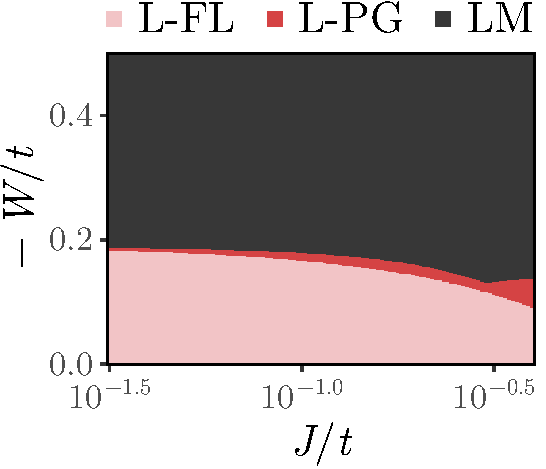
\includegraphics[width=0.32\textwidth]{phaseDiagram.pdf}
	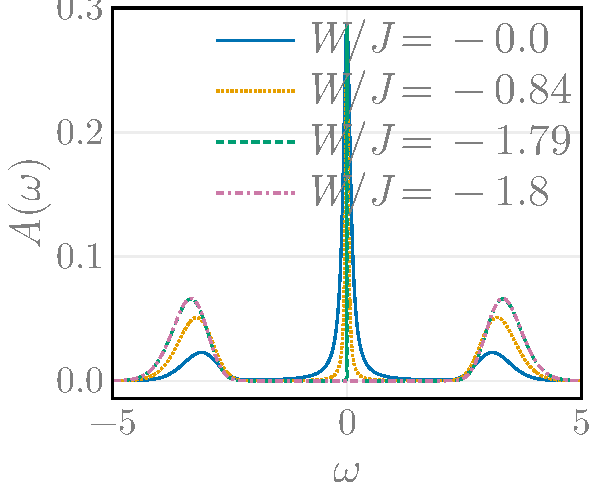
\includegraphics[width=0.32\textwidth]{impSpecFunc_49-1000.pdf}
	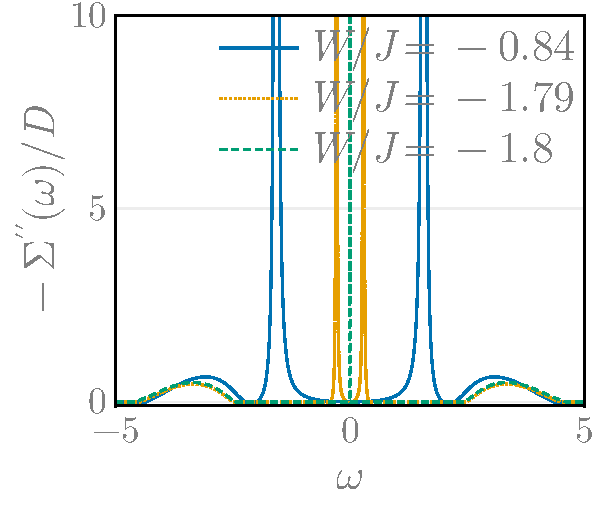
\includegraphics[width=0.32\textwidth]{sigmaImag_49-1000.pdf}
	\caption{{\bf Left}: Zero temperature phase diagram of the embedded impurity model, obtained by tracking impurity-bath spin correlations. The pink phase is characterised by perfect Kondo screening and local Fermi liquid excitations (L-FL), leading to non-zero spin-correlations all over the Fermi surface of the conduction electrons. The red phase is a local pseudogap (L-PG)  phase, where a part of the Fermi surface (starting from the antinodal regions) no longer participates in Kondo screening. This leads to "Fermi arc"-like behaviour in the spin-correlations and the \(k-\)space density of states. The black phase is a local moment (LM) phase, where the impurity is completely decoupled from the conduction electrons. {\bf Middle}: Local spectral function of the impurity site. The blue curve is the normal Kondo resonance in the absence of any bath interaction. The yellow and green curves show the sharpening the spectral function through the locally pseudogapped phase, as momentum states are expelled from the Kondo cloud. The final pink curve shows the charge gap in the local moment phase. {\bf Right:} Imaginary part of impurity self-energy. Poles represent the beginning of the optical gap between the central Kondo resonance and the Hubbard sidebands. Increasing the bath interaction leads to the coalescing of the poles (due to the sharpening of the Kondo resonance), ultimately leading to a zero frequency pole  in the local moment phase.}
	\label{phaseDiagram}
\end{figure}

\subsection{Presence of a local pseuodogapping transition with electronic differentiation in momentum space}
We now discuss the intervening pseudogapped regime (pink region) of the phase diagram. We find that the process of Kondo breakdown in our model occurs anisotropically in our model - the transition starts through the removal, from the Kondo cloud, of the antinodal points of the conduction bath Fermi surface. This is followed by the sequential removal of points away from the antinodes, with the nodal points being removed at the very end. This electronic differentiation is a novel feature of this model that arises because of the more realistic embedding of the impurity site into the conduction bath lattice.

We quantify the removal of these points by the vanishing (up to a tolerance) of the average renormalised scattering probability 
\begin{equation}\begin{aligned}
	\Gamma^*({\bf k}) = \sum_{{\bf q} < \Lambda^*} \left(J^*_{{\bf k}, {\bf q}}\right)^2~,
\end{aligned}\end{equation}
where the other momentum \({\bf q}\) is summed over all the momentum states that reside within the fixed point window. The quantity \(\Gamma({\bf k})\) therefore quantifies the degree to which the state \({\bf k}\) is participating in screening the impurity at low energies. The \(k-\)space forms of this quantity at various values of \(W/J\) is shown in fig.~\ref{gamma_kxky}, and the difference in the behaviour of the nodal and antinodel points is apparent. 

\begin{figure}[!htpb]
	\centering
	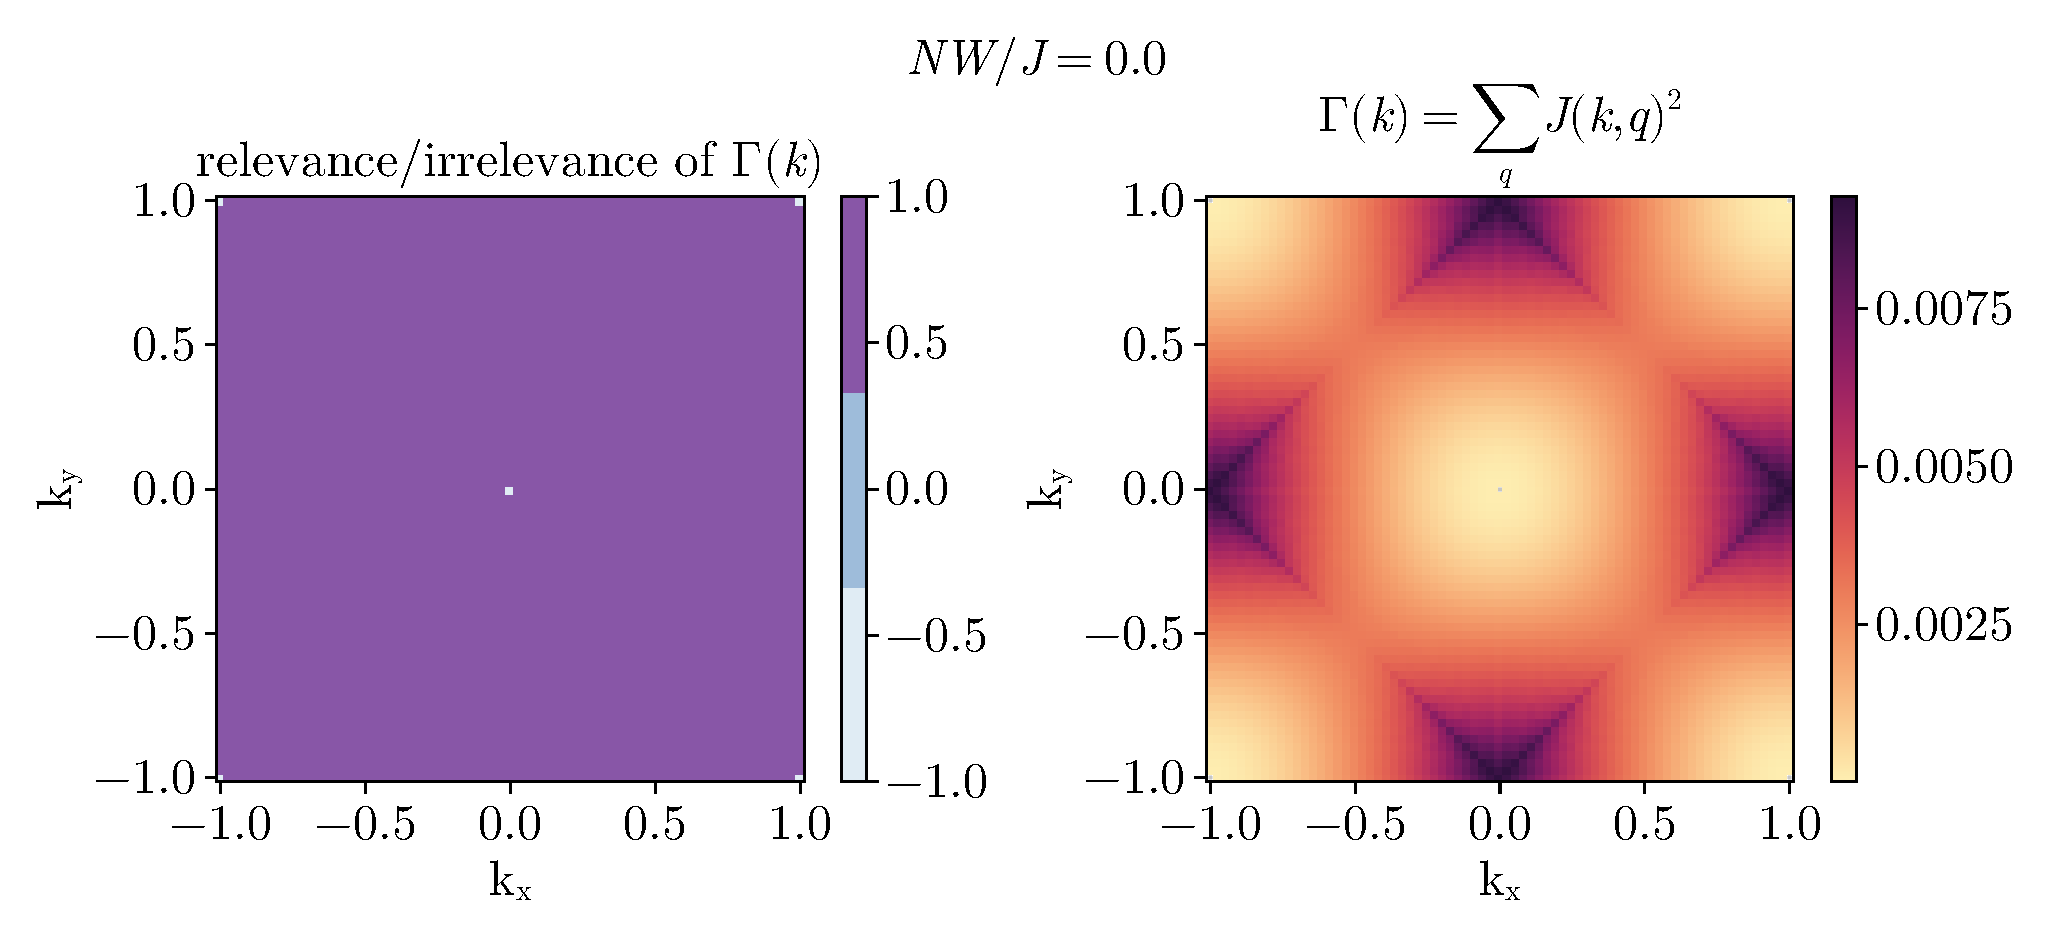
\includegraphics[width=0.23\textwidth]{scattProb-1.pdf}
	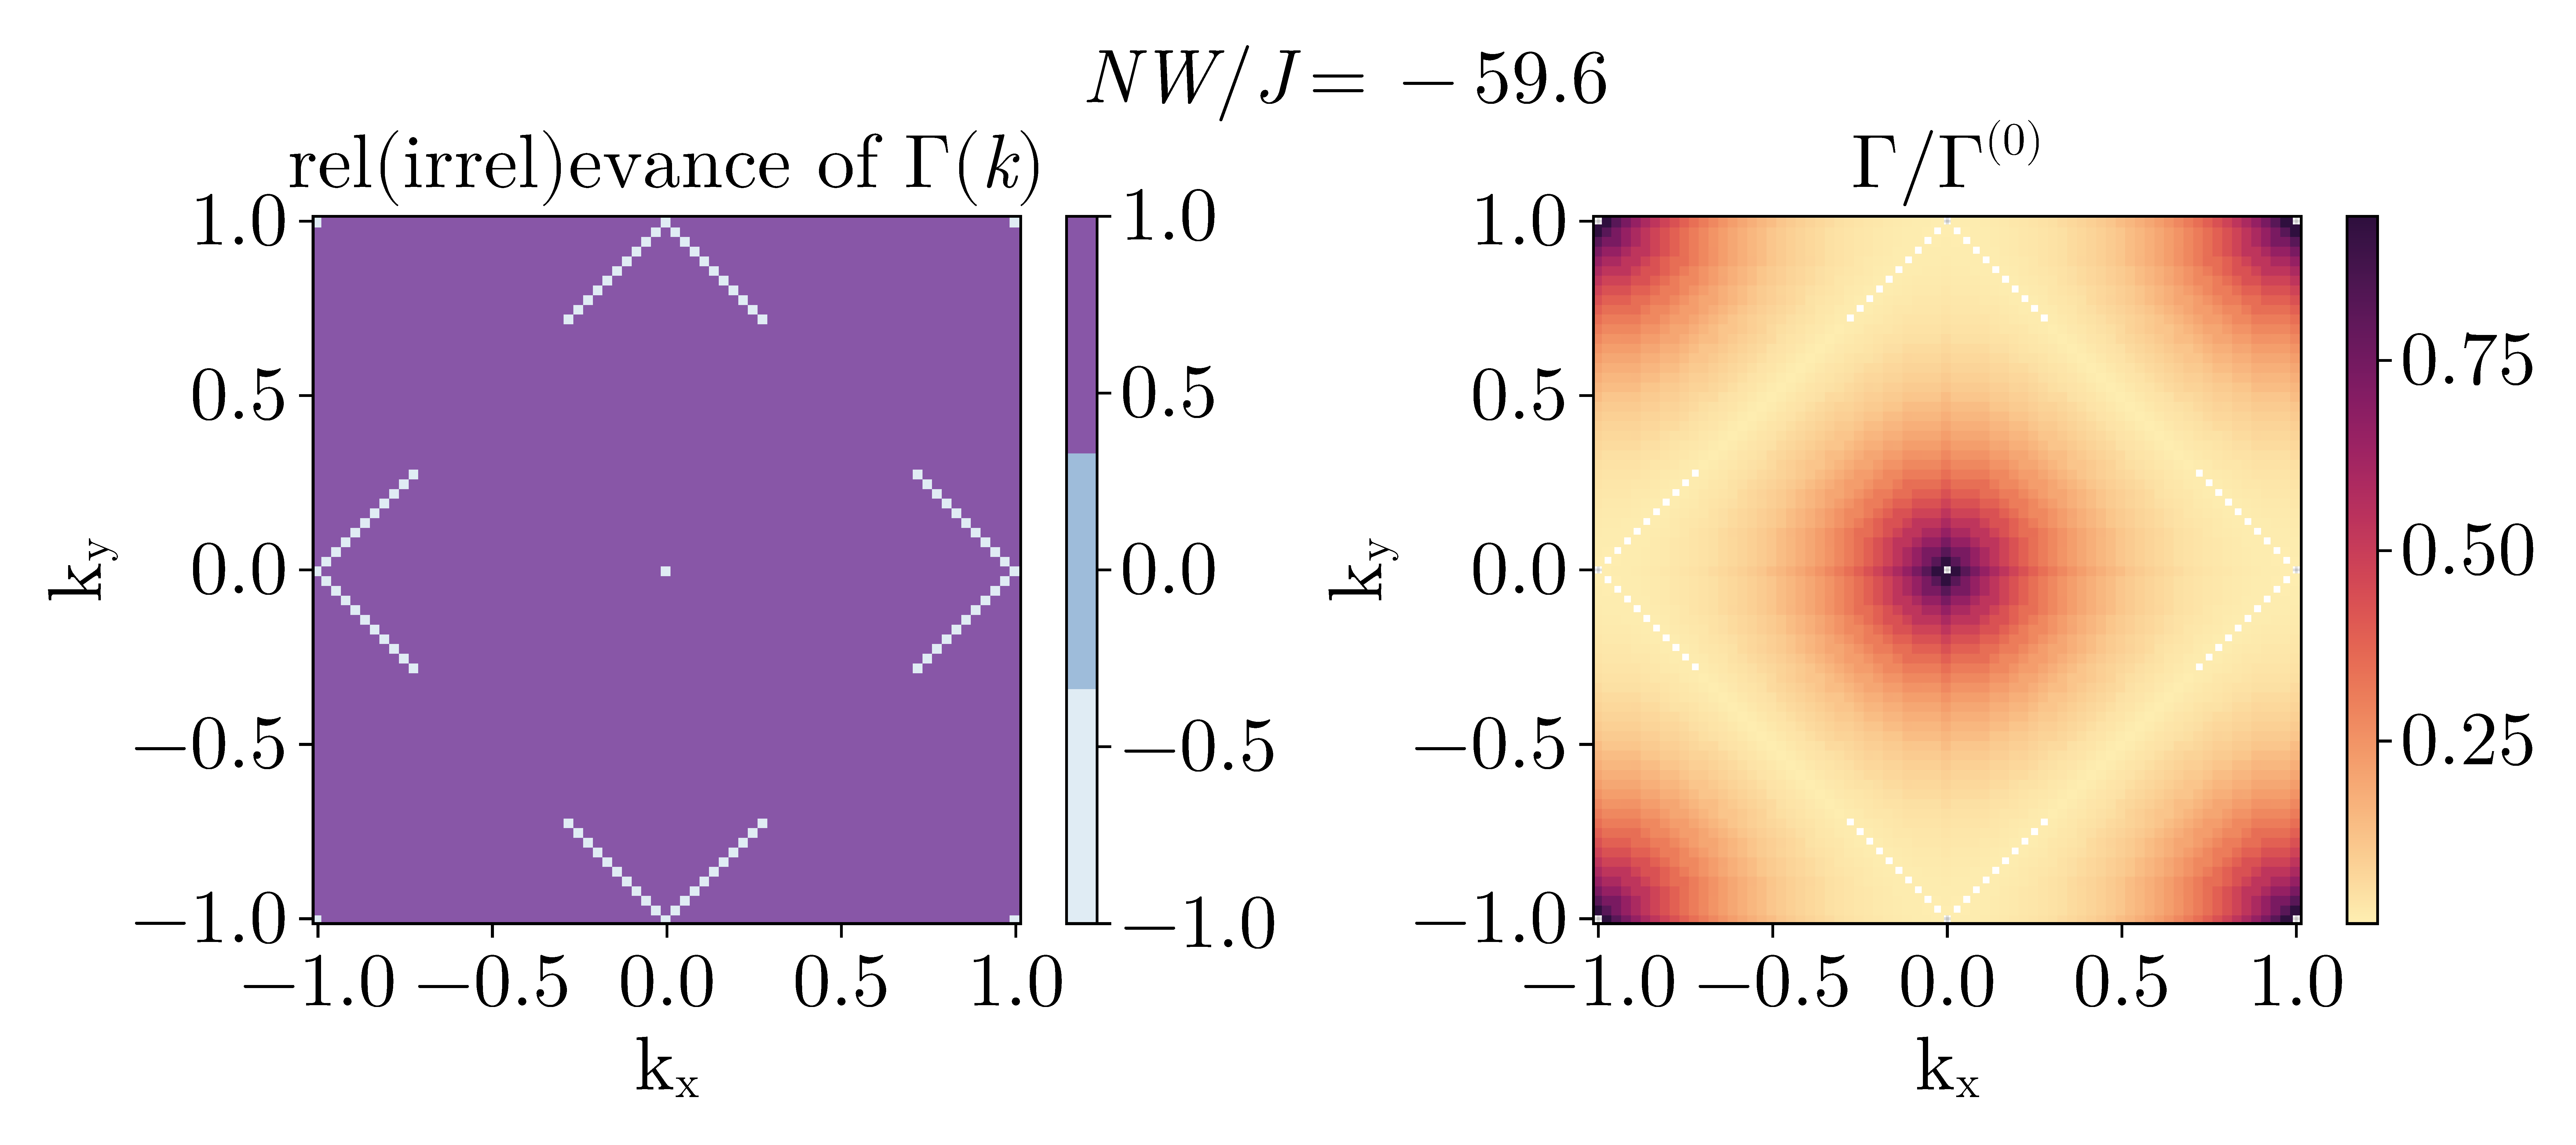
\includegraphics[width=0.23\textwidth]{scattProb-3.pdf}
	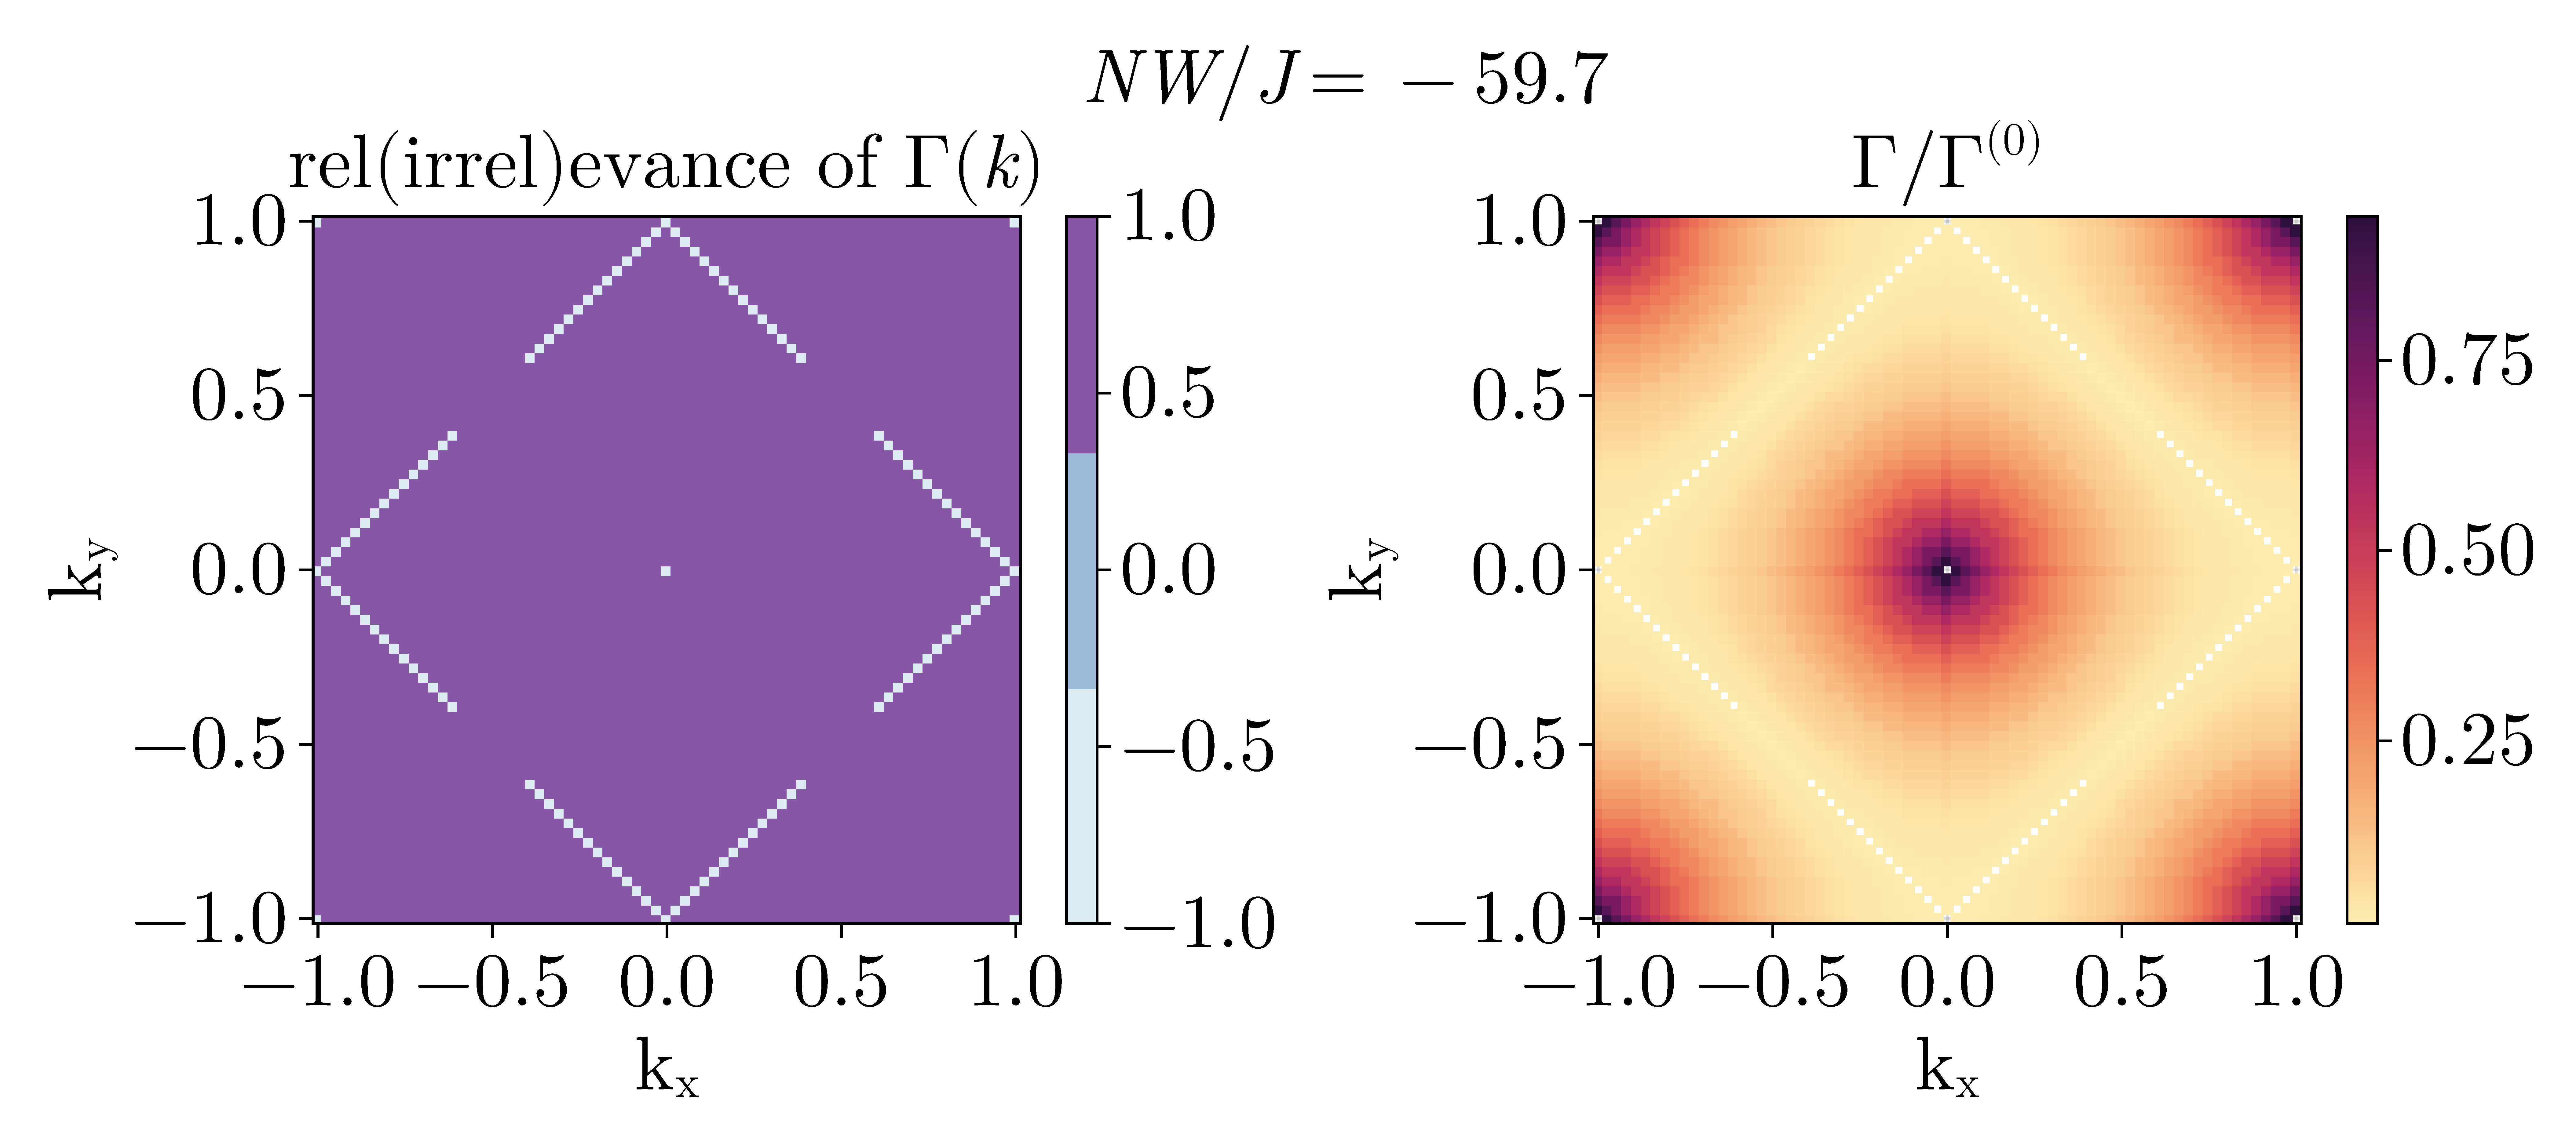
\includegraphics[width=0.23\textwidth]{scattProb-4.pdf}
	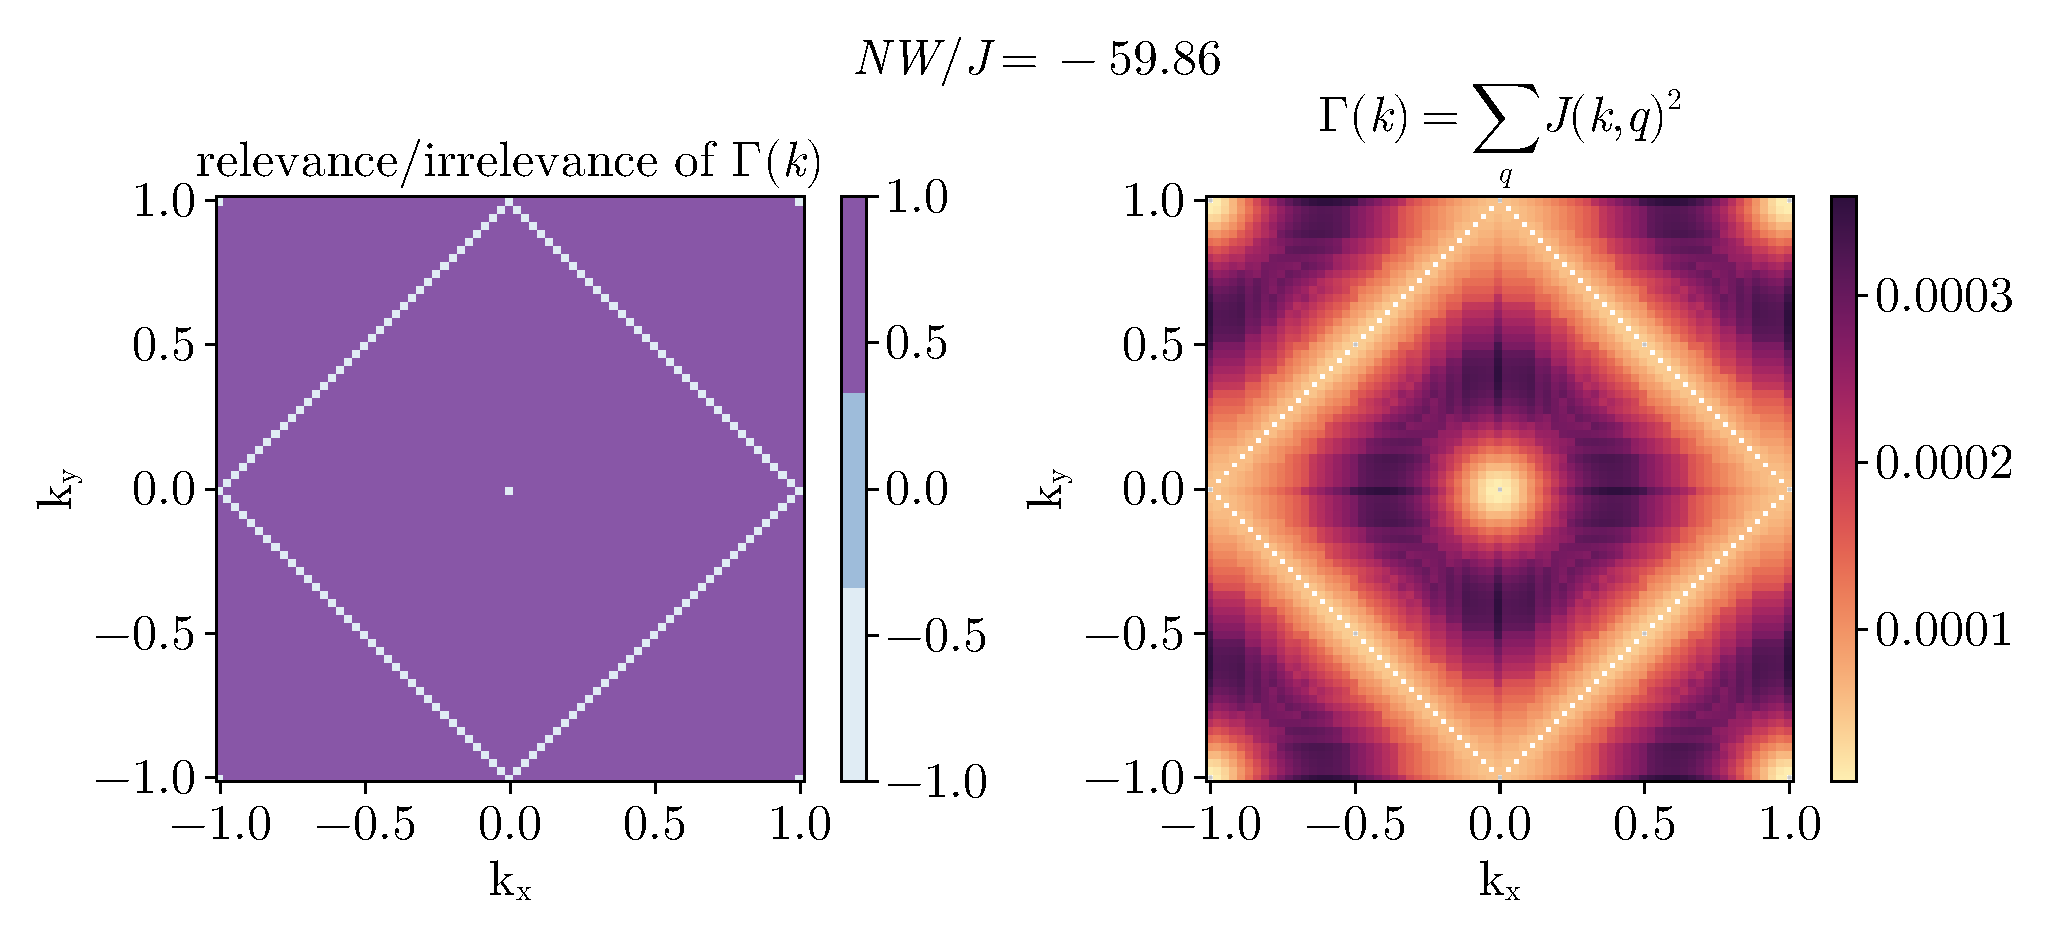
\includegraphics[width=0.23\textwidth]{scattProb-5.pdf}
	\caption{Variation of \(\Gamma\) as \(W/J\) is increased from left to right and top to bottom. Each plot shows whether \(\Gamma({\bf k})\) is relevant (white) or irrelevant (black). The antinodal points are the first state to be removed from the Kondo cloud, while the node is the last to be removed.}
	\label{gamma_kxky}
\end{figure}

\subsection{Spin-correlations across the pseudogap}
In figure ~\ref{spinCorr}, we show the evolution of the spin-flip correlations \(\chi_s(d,\vec k) = \left<S_d^+ S_{\vec k}^- + \text{h.c.}\right>\) in \(k-\)space, as the system is tuned through the pseudogap. At vanishing value of the interaction \(W\), the spin correlations are concentrated around the antinode, because of the \(p-\)wave nature of the Kondo interaction. At the entry into the pseudogap, the correlations become more pronounced near the nodes and become suppressed near the antinodes, signalling that the latter parts will gap out first. The last three figures \((W/J=-1.74, -1.83, -1.84)\) show how \(k-\)points starting from the antinode progressively exit the Kondo cloud, the node being the last to decouple from the impurity.

\begin{figure}[htpb]
	\centering
	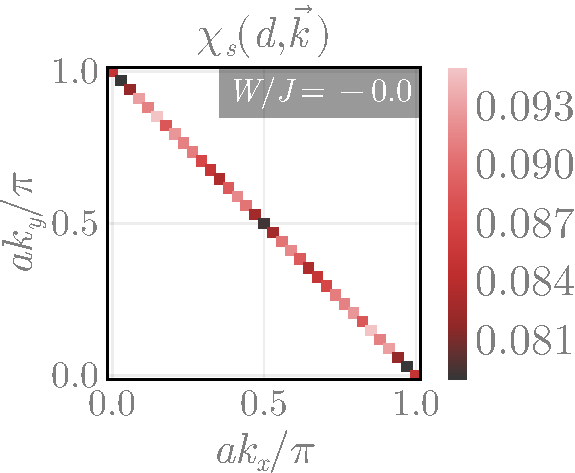
\includegraphics[width=0.23\textwidth]{SF-1.pdf}
	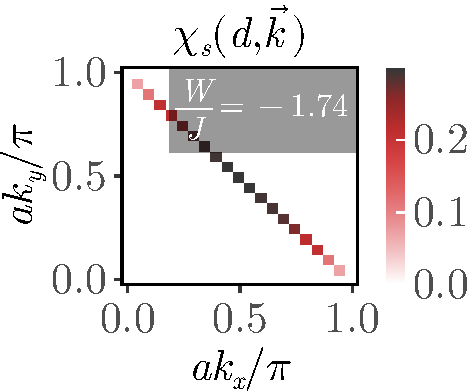
\includegraphics[width=0.23\textwidth]{SF-3.pdf}
	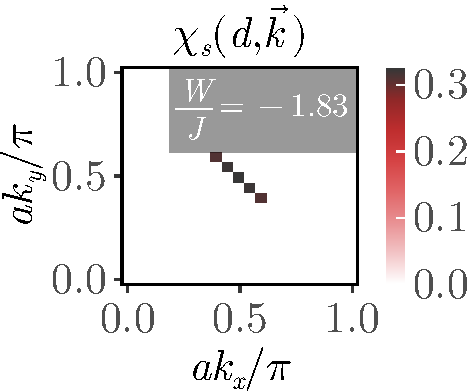
\includegraphics[width=0.23\textwidth]{SF-5.pdf}
	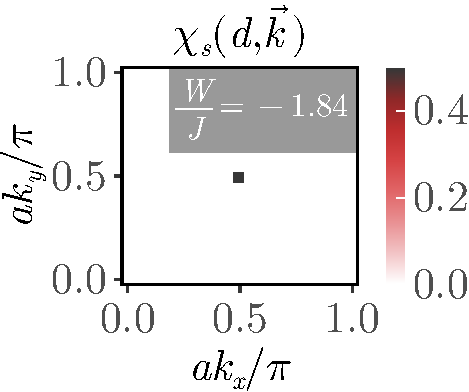
\includegraphics[width=0.23\textwidth]{SF-6.pdf}
	\caption{\(k-\)space distribution of spin-flip scattering correlation \(\chi_s(d,\vec k)\) (defined in the main text). The last three figures \((W/J=-1.74, -1.83, -1.84)\) show how \(k-\)points starting from the antinode progressively exit the Kondo cloud, the node being the last \(k-\)point to decouple from the impurity.}
	\label{spinCorr}
\end{figure}

As a second probe of the pseudogapping phenomenon, we have also studied the entanglement entropy (EE) \(S_\text{EE}(\vec k)\), which is just the von Neumann entropy \(-\text{Tr}\left[\rho \ln \rho\right] \) of the reduced density matrix \(\rho_{\vec k}\) for each \(k-\)state. In accordance with the Kondo spin correlations \(\chi_s\), the EE shows the sequential decoupling, from the impurity, of the antinodes followed by the nodes. 

Studies of \(k-\)space mutual information, \(I_2(\vec k, k_\text{N})\) and \(I_2(\vec k, k_\text{AN})\), between any given \(k-\)state and the node and antinode respectively, have revealed that each point interacts most strongly with it's own neighbourhood (see Supplementary Materials). This feature is in contrast to the charge-transfer correlations in the bath, that show ``long-ranged" interactions between the node and the antinode. These correlations will be discussed immediately after this, and are primarily responsible for driving the impurity transition and destabilising the Kondo cloud.

\subsection{Charge correlations}
In order to study the mechanism behind the destabilisation of the Kondo cloud through the pseudogap, we calculate the \(k-\)space double occupancy \(\left<n_{\vec k \uparrow} n_{\vec k \downarrow}\right>\) and \(k-\)space charge-transfer correlation \(\chi_c(\vec k, \vec q) = \left<c^\dagger_{\vec k \uparrow} c^\dagger_{\vec k \downarrow} c_{\vec q \downarrow}c_{\vec q \uparrow}\right>\) (Fig.~\ref{cfnode}). We find that the entry into the pseudogap is marked by an increase of doubly-occupied states near the antinode in comparison to \(W=0\). These pairs likely lead to the concomitant vanishing of spin-correlations near the antinode at the same value of \(W\), as seen in Fig.~\ref{spinCorr}. More insight on the nature of these correlations are obtained from the fluctuations \(\chi_c(\vec k, \vec q)\) starting from the node \((\vec q = k_\text{N})\) and antinode \(\left( \vec q = k_\text{AN}\right) \). Interestingly, we find strong pair-transfer interactions between the node and antinode. Within the pseudogap, this leads to charge-isospin flip correlations between the decoupled antinodal region and the still-coupled nodal region.
\begin{figure}[!htpb]
	\centering
	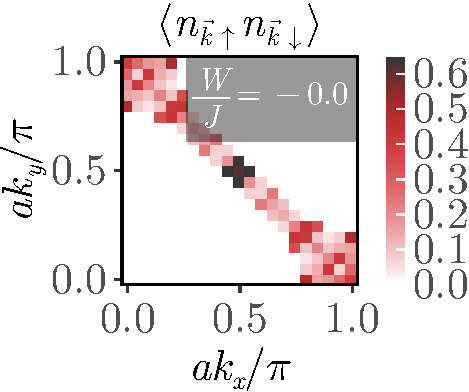
\includegraphics[width=0.23\textwidth]{doubOcc-1.pdf}
	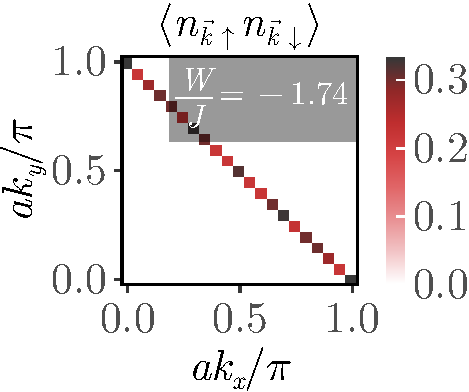
\includegraphics[width=0.23\textwidth]{doubOcc-3.pdf}
	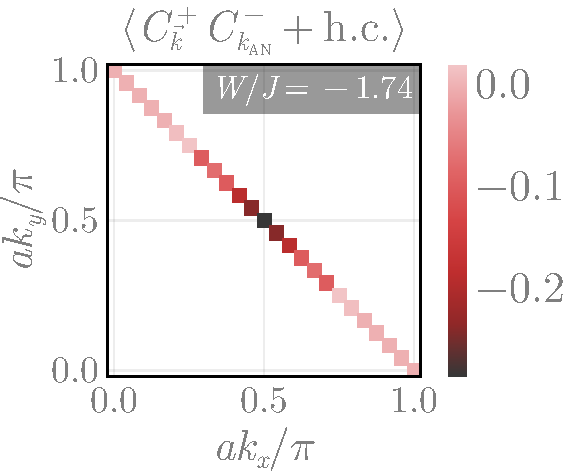
\includegraphics[width=0.23\textwidth]{cfantinode-3.pdf}
	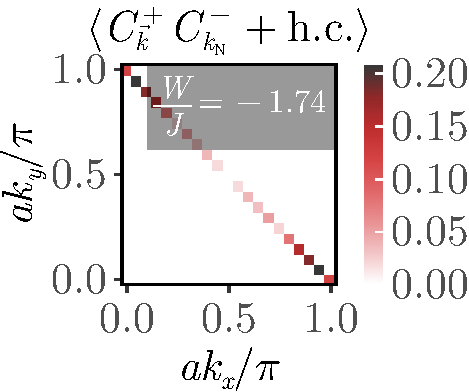
\includegraphics[width=0.23\textwidth]{cfnode-3.pdf}
	\caption{{\it Top panels}: Distribution of double occupancy at \(W=0\) and \(W=-1.74\) (entry into the pseudogap). While the double occupancy is concentrated near the nodes at \(W=0\), it rises near the antinodes at the start of the pseudogap, signalling its destabilisation. {\it Bottom panels}: Charge-transfer correlation \(\chi_c\) (defined in main text) starting from antinode (left) and node (right), at the beginning of the pseudogap phase. Strong node-antinode correlations are clearly visible.}
	\label{cfnode}
\end{figure}

\subsection{Emergence of a two-channel Kondo Model as the low-energy theory in the pseudogap phase}
As the bath interaction \(W\) is tuned through the L-PG phase, the four nodal points in the Brillouin zone are the last to decouple from the impurity. This allows us to write down a simpler Kondo model near the transition, focusing on scattering processes involving the nodal region. Specifically, for the Kondo term \(J_{{\bf k}_1, {\bf k}_2})\), we find that only the following classes of scattering processes survive close to the critical point:
\begin{itemize}
	\item Both momenta in a neighbourhood around \({\bf k}_N\), where \({\bf k}_N\) can be any of the four nodal points,
	\item One momentum from the neighbourhood around \({\bf k}_N\), while the other from the neighbourhood around \({\bf k}_N + \left( \pi, \pi \right) \)~.
\end{itemize}
The second class is tied to the first through a symmetry of the Hamiltonian (eq.~\ref{hamiltonanSymms}). The crucial feature of these processes is that each node only interacts with the other node directly opposite to it across the origin. That is, \(\left(\pi/2, \pi/2\right) \) and \(\left(-\pi/2, -\pi/2\right) \) only interact between themselves, while \(\left(\pi/2, -\pi/2\right) \) and \(\left(-\pi/2, \pi/2\right) \) form their own pair of connected regions. 

Let \(S^\pm\) be the set of momentum states in a small window around nodes along \(k_x = \pm k_y\). As discussed immediately above, the Kondo spin-exchange term close to the transition does not lead to scattering of any \(k-\)state from \(S^+\) to \(S^-\). This is verified by calculating the ratio \(\text{max}\left\{ J_{k^+_1, k^-_2} \right\} / \text{max}\left\{ J_{k^+_1, k^+_2} \right\}\), where the maximum in the numerator is calculated from all the low-energy (fixed point) Kondo scattering processes that connect the two sets \(S^\pm\), while the denominator maximum is from within the set \(S^+\). This ratio vanishes (left panel of Fig.~\ref{channelDecoupling}) within the local pseudogap regime, indicating that no direct Kondo scattering process persists between the two sectors \(S^\pm\) at low energies, deep within the pseudogap regime.

\begin{figure}[htpb]
	\centering
	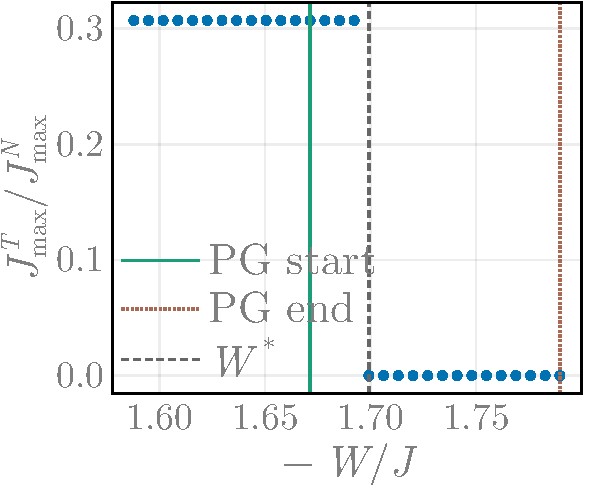
\includegraphics[width=0.45\textwidth]{quadrantMaxKondo-49.pdf}
	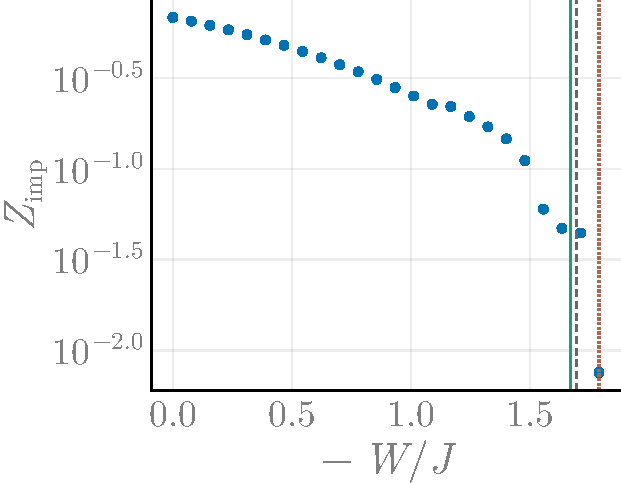
\includegraphics[width=0.45\textwidth]{localQPResidue.pdf}
	\caption{Left: Ratio between the maximum values of the fixed point values of the Kondo couplings for scattering processes between and within the regions \(S^+\) and \(S^-\). The vanishing of the fixed point ratio indicates that the pseudogap regime features a singular low-energy effective theory, where the Fermi surface neighbourhood splits into two disconnected regions with no explicit term in the Hamiltonian connecting them directly. Right: The quasiparticle residue \(Z_\text{imp}\) of the local gapless excitations in various regions. The vanishingly small values of \(Z_\text{imp}\) lend more support to the two-channel (and hence the non-Fermi liquid) nature of the low-energy physics in the pseudogap regime.}
	\label{channelDecoupling}
\end{figure}

The decoupling of the \(k-\)space regions \(S^\pm\) is captured by the following simplified low-energy Hamiltonian:
\begin{equation}\begin{aligned}\label{twoChannel}
H_\text{eff} = H(S^+) + H(S^-);~H(S) = \sum_{{\bf q}\in S,\sigma}\varepsilon_{\bf q}c^\dagger_{{\bf q}\sigma}c_{{\bf q}\sigma} + \sum_{{\bf q}_1\in S,{\bf q}_2\in S}\sum_{\alpha,\beta}J^*({\bf q}_1,{\bf q}_2){\bf S}_d\cdot {\bf \sigma}_{\alpha\beta}c^\dagger_{{\bf q}_1\alpha}c_{{\bf q}_2\beta}~,
\end{aligned}\end{equation}
where \(H(S^\pm)\) represents the dynamics of momentum states residing in regions \(S^\pm\). The only source of information transfer between the two regions is the fact that they interact with the same impurity local moment.

Eq.\ref{twoChannel} tells us that the low-energy dynamics of the embedded eSIAM close to the Kondo-breakdown transition is governed by an emergent {\bf two-channel Kondo model}, with the conduction bath states in the sets \(S^\pm\) making up the two channels. It is well-known that the two-channel Kondo model hosts non-Fermi liquid excitations at low-energies; this is also corroborated by our calculations of the quasiparticle residue \(Z_\text{imp}\) for the local gapless excitations. For a single-particle Greens function of an interacting model, the quasiparticle residue \(Z\) is defined as
\begin{equation}\begin{aligned}
	G = Z G^{(0)} + G_\text{inc}~,
\end{aligned}\end{equation}
where \(G^{(0)}\) is the non-interacting Greens function and \(G_\text{inc}\) is contribution to the Greens function arising from incoherent short-lived excitations. Small values of \(Z\) indicate that the excitations cannot be described in terms of a Fermi liquid theory. Indeed, as shown in the right panel of Fig.~\ref{channelDecoupling}, the quasiparticle residue \(Z_\text{imp}\) of the impurity excitations becomes vanishingly small in the pseudogap region, signalling that the excitations are of a non-Fermi liquid nature.

Given that this is a critical point in the impurity model phase diagram (separating the local Fermi liquid and local moment phases), it is not surprising that a quantum critical model emerges at that point. Signatures of the quantum critical nature include power-law divergence in various correlation functions as temperature \(T \to 0\), and non-Fermi liquid excitations replacing the local Fermi liquid.

\section{Journey Through the Pseudogap on The Lattice model}
We have already seen from the lattice-embedded impurity model that the impurity phase transition is anisotropic in \(k-\)space. This has consequences for the metal-insulator transition of the lattice model. We now describe, in terms of correlations, how the Fermi surface of the lattice model is destabilised when the system is tuned through the pseudogap. For this, we employ the relations we derived between correlations on the impurity model and those on the lattice model.

\subsection{\(k-\)space spectral function and self-energy}
The primary indicator of the pseudogapping nature of the transition is of course the \(k-\)space density of states or the spectral function, shown in Fig.~\ref{tiledSpecFunc}. For \(W=0\), all points on the Fermi surface are gapless. As we enter the pseudogap, the region around the antinodes lose all spectral weight and become gapped. Increasing the value of \(W\) further leads to the enlargement of the gapped region; exactly at the transition, we end up with a singular Fermi surface composed of just the nodal points.

This is also supported by our computations of the \(k-\)space self-energy. We show the zero frequency value of the \(k-\)space self-energy in Fig.~\ref{selfenergy}. This is computed from using Dyson's equation \(\Sigma_k = 1/G_k^{(0)} - 1/G_k\), where \(G_k\) is the interacting \(k-\)space Greens function while \(G_k^{(0)}\) is the non-interacting \(W=0\) Greens function. We find that the beginning of the pseudogap is marked by poles in the self-energy at the antinodal points; at the transition, only the nodes display vanishing self-energy at zero frequency.
\begin{figure}[htpb]
	\centering
	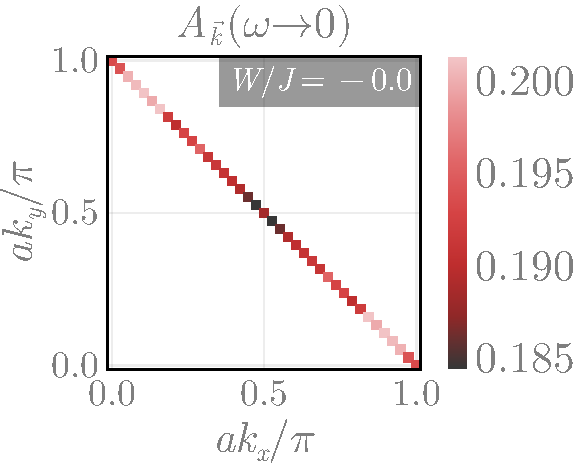
\includegraphics[width=0.23\textwidth]{kspaceDOS-1.pdf}
	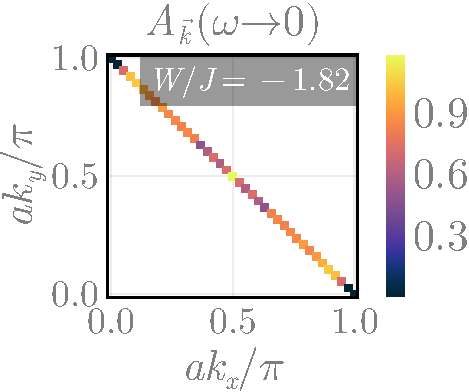
\includegraphics[width=0.23\textwidth]{kspaceDOS-2.pdf}
	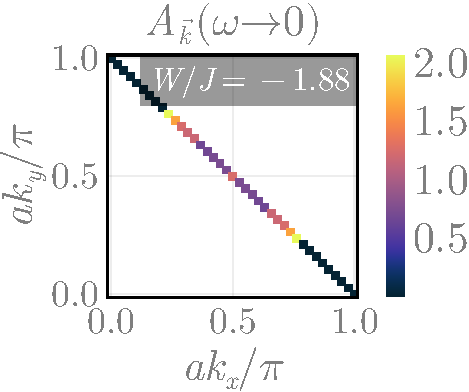
\includegraphics[width=0.23\textwidth]{kspaceDOS-3.pdf}
	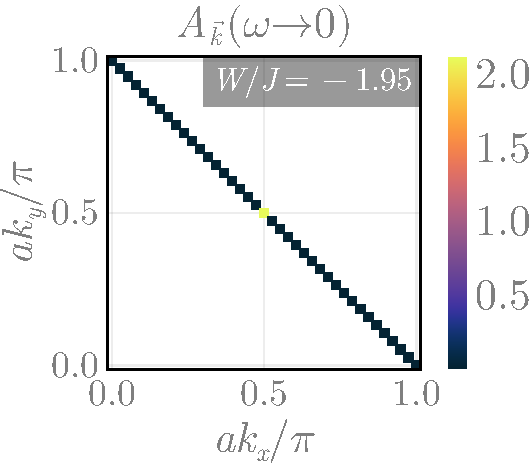
\includegraphics[width=0.23\textwidth]{kspaceDOS-4.pdf}
	\caption{One-particle \(k-\)space spectral function. In the absence of bath interactions, all points on Fermi surface are gapless (first panel). Proceeding through the pseudogap results in the gapping out of Fermi surface points starting from the antinode (second panel) and approaching the node (third panel), until finally only the node remains at the critical point (fourth panel).}
	\label{tiledSpecFunc}
\end{figure}
\begin{figure}[htpb]
	\centering
	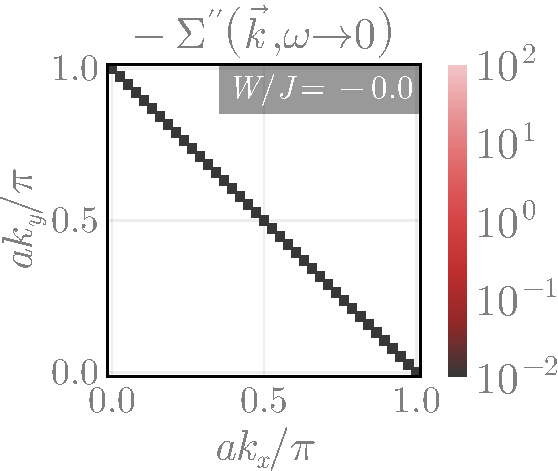
\includegraphics[width=0.23\textwidth]{selfEnergyKspace-1.pdf}
	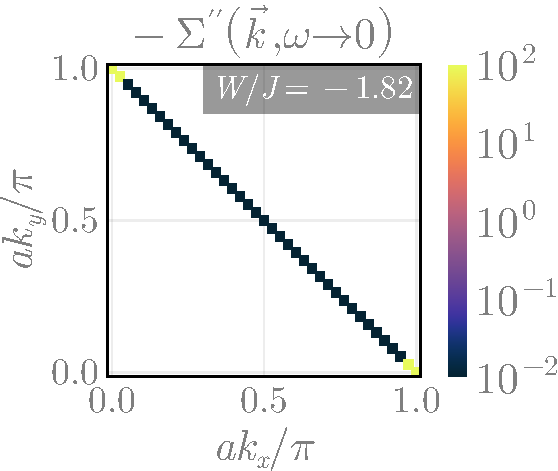
\includegraphics[width=0.23\textwidth]{selfEnergyKspace-2.pdf}
	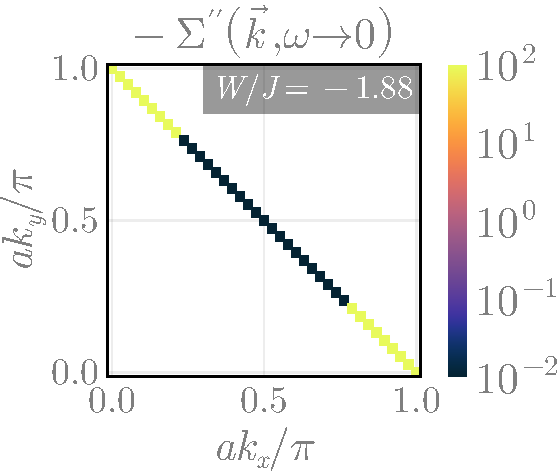
\includegraphics[width=0.23\textwidth]{selfEnergyKspace-3.pdf}
	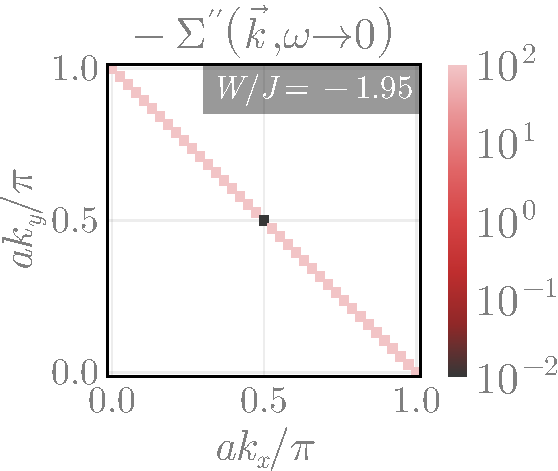
\includegraphics[width=0.23\textwidth]{selfEnergyKspace-4.pdf}
	\caption{\(k-\)space self-energy. For \(W=0\), the self-energy is vanishingly small, leading to a Fermi liquid phase described by well-defined quasiparticles. Inside the pseudogap, the self-energy diverges near the antinodes, leading to their gapping. The coexistence of gapped and gapless points on the Fermi surface in the pseudogapped region leads to non-Fermi liquid behaviour of the gapless excitations, as captured by the emergent two-channel behaviour within the impurity model. The metal at the transition is supported only the four nodal points.}
	\label{selfenergy}
\end{figure}

\subsection{Momentum-space spin-correlations}
We first look at static spin correlations \(\chi_s(k_1, k_2) = \frac{1}{2}\left<S_{k_1}^+ S_{k_2}^- + \text{h.c.} \right>\). These processes correspond to the gapless excitations of the Fermi liquid phase. We find that 
\begin{figure}[htpb]
	\centering
	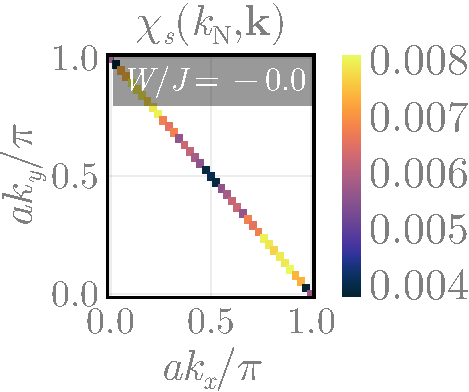
\includegraphics[width=0.24\textwidth]{tiledSF-1.pdf}
	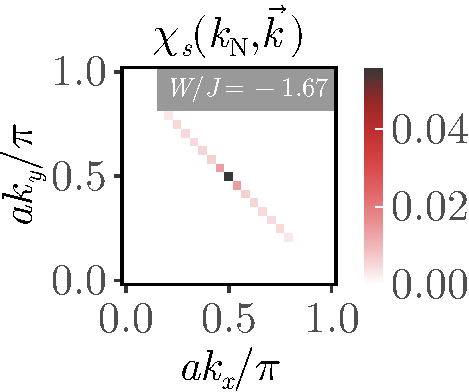
\includegraphics[width=0.24\textwidth]{tiledSF-2.pdf}
	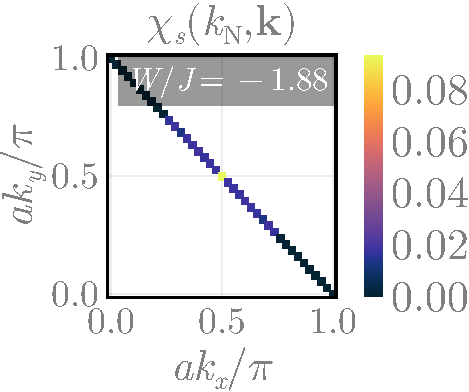
\includegraphics[width=0.24\textwidth]{tiledSF-3.pdf}
	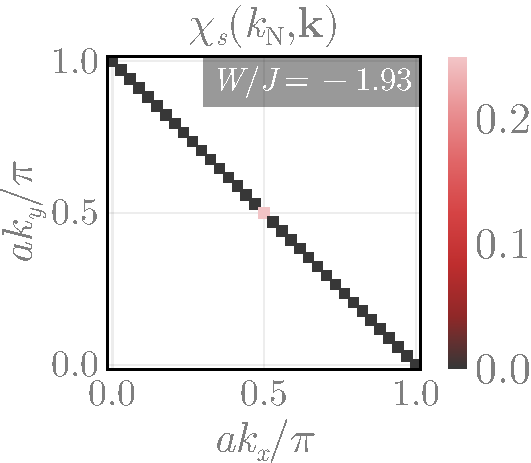
\includegraphics[width=0.24\textwidth]{tiledSF-4.pdf}
	\caption{Spin-flip correlations \(\left<S(k_N)^+, S({\bf k})^-\right>\) between the nodal point \(k_N = \left( -\pi/2, -\pi/2\right)\) and an arbitrary \(k-\)point on the Fermi surface. In the absence of bath interaction (first panel), the correlations are somewhat uniformly distributed along the Fermi surface. As we enter the pseudogap (second panel), the spin-correlations near the antinode vanish, indicating that they have been removed from the metallic excitations. Passing through the pseudogap involves in the extensions of the gapped region (third panel), until finally only the node remains (fourth panel).}
	\label{tiledSF}
\end{figure}

\subsection{Entanglement entropy and Mutual information}
\begin{figure}[htpb]
	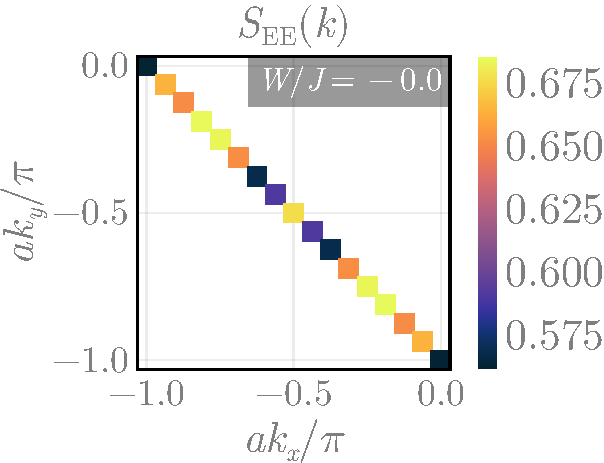
\includegraphics[width=0.24\textwidth]{S_k-1.pdf}
	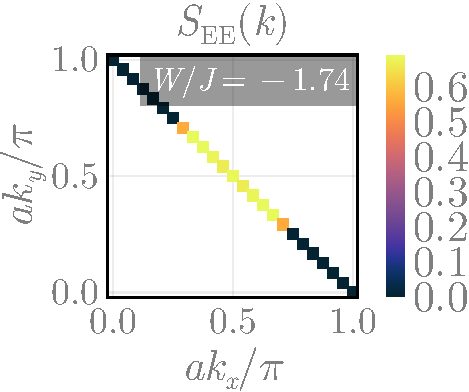
\includegraphics[width=0.24\textwidth]{S_k-3.pdf}
	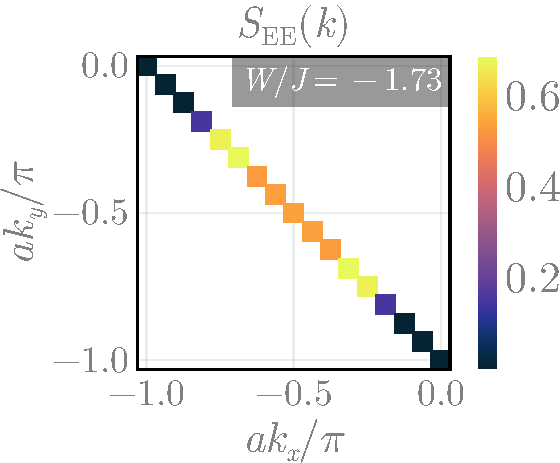
\includegraphics[width=0.24\textwidth]{S_k-4.pdf}
	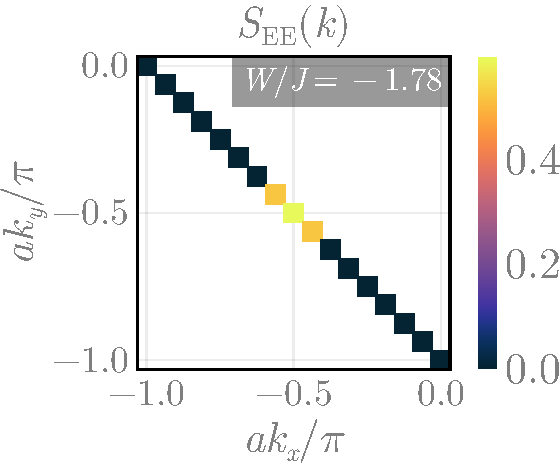
\includegraphics[width=0.24\textwidth]{S_k-5.pdf}
\end{figure}
\begin{figure}[htpb]
	\centering
	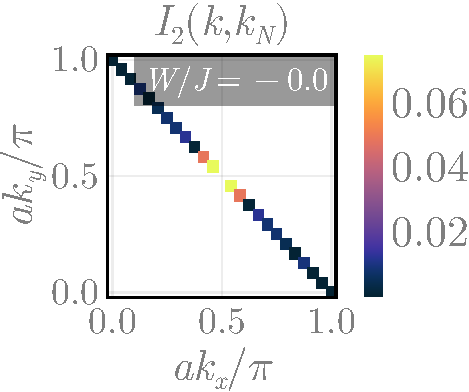
\includegraphics[width=0.24\textwidth]{I2_k_N-1.pdf}
	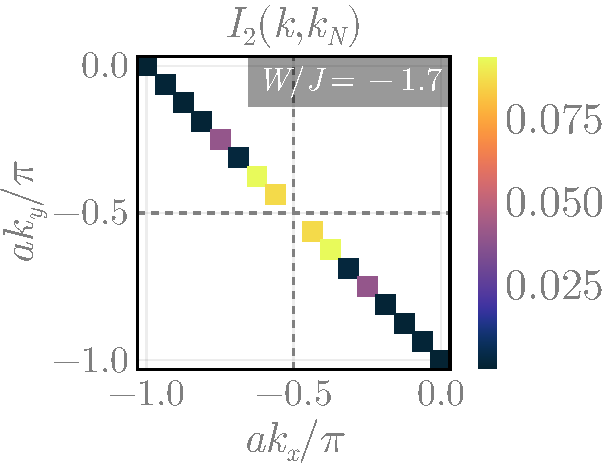
\includegraphics[width=0.24\textwidth]{I2_k_N-3.pdf}
	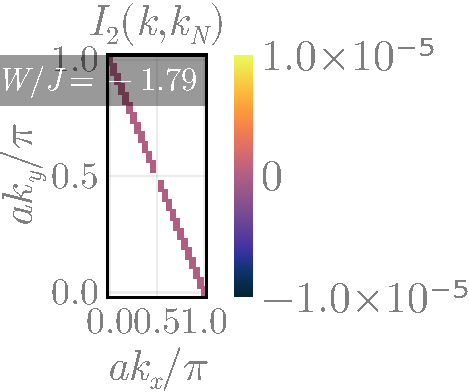
\includegraphics[width=0.24\textwidth]{I2_k_N-4.pdf}
	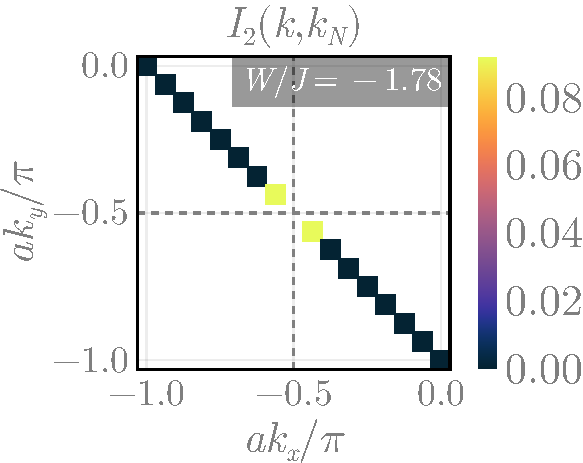
\includegraphics[width=0.24\textwidth]{I2_k_N-5.pdf}
\end{figure}
\begin{figure}[htpb]
	\centering
	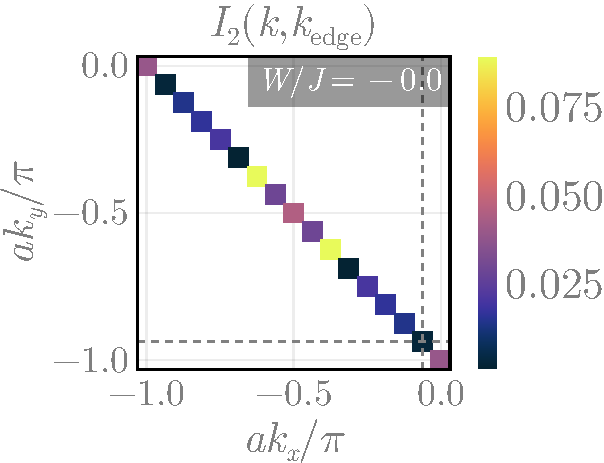
\includegraphics[width=0.24\textwidth]{I2_k_edge-1.pdf}
	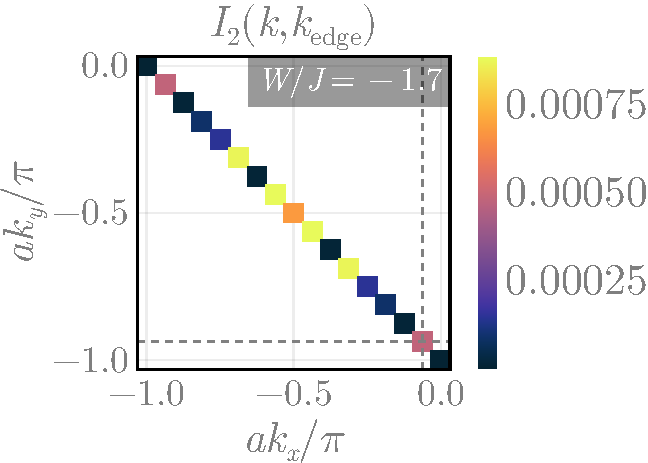
\includegraphics[width=0.24\textwidth]{I2_k_edge-3.pdf}
	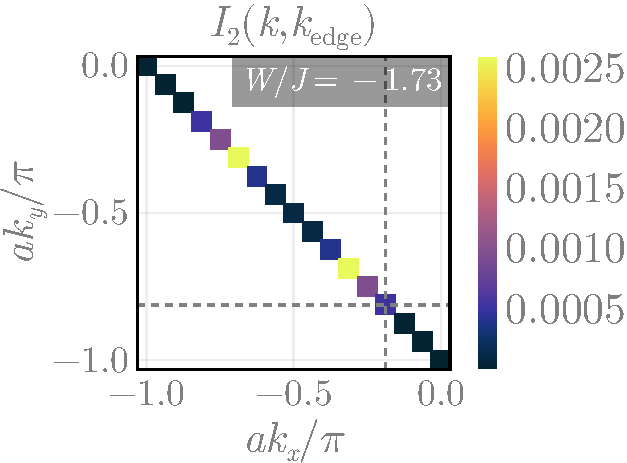
\includegraphics[width=0.24\textwidth]{I2_k_edge-4.pdf}
	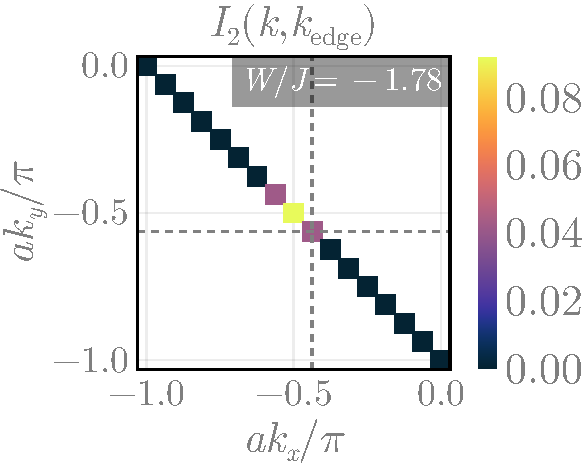
\includegraphics[width=0.24\textwidth]{I2_k_edge-5.pdf}
\end{figure}


\subsection{Heisenberg model as a low-energy description of the insulator}

In the insulating phase, the ground state of each auxiliary model hosts a decoupled local moment. Upon applying the tiling procedure, the lattice model ground state becomes that of the Hubbard model in the atomic limit. In order to lift the extensive degeneracy of the state, we will now take into consideration inter-auxiliary model virtual scattering processes that were subdominant in the metallic phase and were hence ignored. These one-particle scattering processes lead to the emergence of a nearest-neighbour superexchange interaction.

For simplicity, we consider two impurity sites labelled \(1\) and \(2\) associated with two nearest-neighbour auxiliary models. The ground state subspace is four-fold degenerate:
\begin{equation}\begin{aligned}
	\ket{\Psi_L} = \left\{\ket{\sigma_1,\sigma_2}\right\}~,\quad \sigma_i = \pm 1
\end{aligned}\end{equation}
where \(\sigma_i\) is the spin state of site \(i\). This ground state is derived from the following "zeroth order" Hamiltonian that emerges in the local moment phase of the auxiliary models when all scattering processes between the impurity and conduction bath are RG-irrelevant:
\begin{equation}\begin{aligned}
	H_0 = -\frac{U}{2}\sum_{i=1,2}\left(n_{i \uparrow} - n_{i \downarrow}\right)^2~;
\end{aligned}\end{equation}
the local correlation on the impurity site becomes the largest scale in the problem in this phase and pushes the \(\ket{n_i=2}\) and \(\ket{n_i=0}\) states to high energies. This then defines the high-energy subspace for our calculation:
\begin{equation}\begin{aligned}
	\ket{\Psi_H} = \ket{C_1,C_2}~,
\end{aligned}\end{equation}
where \(C_i\) can take values 0 or 2, indicating that the state \(i\) is either empty or full, respectively. Both the double and hole states exist at a charge gap of the order of \(U/2\) above the low-energy singly-occupied subspace defined by the states \(\ket{\Psi_L}\).

In order to allow virtual fluctuations that can lift the large ground state degeneracy and lower the energy, we consider (perturbatively) the effects of an irrelevant single-particle hybridisation that connects the nearest-neighbour sites. This perturbation Hamiltonian is therefore of the form
\begin{equation}\begin{aligned}
	H_t = \sum_\omega V(\omega) \mathcal{P}(\omega)~\sum_\sigma\left(c^\dagger_{1\sigma}c_{2\sigma} + \text{h.c.}\right) ~,
\end{aligned}\end{equation}
where \(V(\omega)\) only acts on states at the energy scale \(\omega\); the renormalisation of \(V\) is encoded in the fact that \(V(\omega)\) is largest for the excited states and vanishes at low-energies: \(V(\omega \to 0) = 0\).

In order to obtain a low-energy effective Hamiltonian for the impurity sites arising from this hybridisation, we integrate out \(H_t\) via a Schrieffer-Wolff transformation. This leads to the following second-order Hamiltonian:
\begin{equation}\begin{aligned}
	H_\text{eff} = \mathcal{P}_L H_t G\mathcal H_t \mathcal{P}_L~.
\end{aligned}\end{equation}
The operator \(\mathcal{P}_L\) projects onto the low-energy subspace \(\ket{\Psi_L}\) - this ensures that we remain in the low-energy subspace at the beginning and at the end of the total process. The Greens function \(G = (E_L - H_0)^{-1}\) incorporates the excitation energy to go from the low-energy subspace \(\ket{\Psi}_L\) (of energy \(E_L\)) to the excited subspace \(\ket{\Psi}_H\) of energy \(E_L + U/2\). Substituting the form of the perturbation Hamiltonian and the excitation energy into the above expression gives
\begin{equation}\begin{aligned}\label{effHam1}
	H_\text{eff} = \frac{V_H^2}{-U/2}\sum_{\sigma,\sigma^\prime} \left[c^\dagger_{1\sigma}c_{2\sigma}c^\dagger_{2\sigma^\prime}c_{1\sigma^\prime} + c^\dagger_{2\sigma}c_{1\sigma}c^\dagger_{1\sigma^\prime}c_{2\sigma^\prime}\right] ~.
\end{aligned}\end{equation}
where \(V_H \equiv V(\omega \to U/2)\) is the impurity-bath hybridisation at energy scales of the order of the Mott gap, in the sense of an RG flow. Terms with consecutive creation or annihilation operators on the same site are prohibited because each site is singly-occupied in the ground state. It is now easy to cast this Hamiltonian into a more recognizable form. For \(\sigma^\prime=\sigma\), we get
\begin{equation}\begin{aligned}
	\sum_{\sigma}\delta_{\sigma,\sigma^\prime}c^\dagger_{1\sigma}c_{2\sigma}c^\dagger_{2\sigma^\prime}c_{1\sigma^\prime} = \sum_\sigma \left(n_{1\sigma} - n_{1\sigma}n_{2\sigma}\right) ~,
\end{aligned}\end{equation}
while \(\sigma=-\sigma^\prime=\pm 1\) gives 
\begin{equation}\begin{aligned}
	\sum_{\sigma}\delta_{\sigma,-\sigma^\prime}c^\dagger_{1\sigma}c_{2\sigma}c^\dagger_{2\sigma^\prime}c_{1\sigma^\prime} = -\left(S_1^+ S_2^- + \text{h.c.}\right)~.
\end{aligned}\end{equation}
For the latter expression, we introduced the local spin-flip operators \(S_i^\pm\). The expression above it can also be cast into spin variables, using the equations
\begin{equation}\begin{aligned}
	\frac{1}{2}\sum_{\sigma}n_{i\sigma} = \frac{1}{2},\\
    \frac{1}{2}\sum_{\sigma}\sigma n_{i\sigma} = S_i^z,
\end{aligned}\end{equation}
where the first equation is simply the condition of half-filling at each site, and the second equation is the definition of the local spin operator in \(z-\)direction. Adding and subtracting the equations gives \(n_{i\sigma} = \frac{1}{2} + \sigma S_i^z\)~.

Substituting everything back into eq.~\ref{effHam1} and dropping constant terms gives
\begin{equation}\begin{aligned}
	H_\text{eff} = 2\frac{V_H^2}{U/2}\left(2S_1^z S_2^z + S_1^+S_2^- + S_1^-S_2^+\right) = J_\text{eff} {\bf S}_1\cdot{\bf S}_2~,
\end{aligned}\end{equation}
where the effective antiferromagnetic Heisenberg coupling is \(J_\text{eff} = \frac{8V_H^2}{U}\).







\clearpage



\section{The Mott MIT: a local perspective}
\subsection{Gapping of the local spectral function and vanishing of correlations}
% At a critical value \(U_b = -J/4\) of the local correlation \(U_b\) on the bath zeroth site, the couplings \(J\) and \(V\) of the auxiliary model become irrelevant while \(U\) becomes remains non-zero, leading to a low-energy phase where the impurity is cut off from the conduction bath. This is the local moment phase, where low-energy excitations have been gapped out.
% \begin{figure}[htpb]
% 	\centering
% 	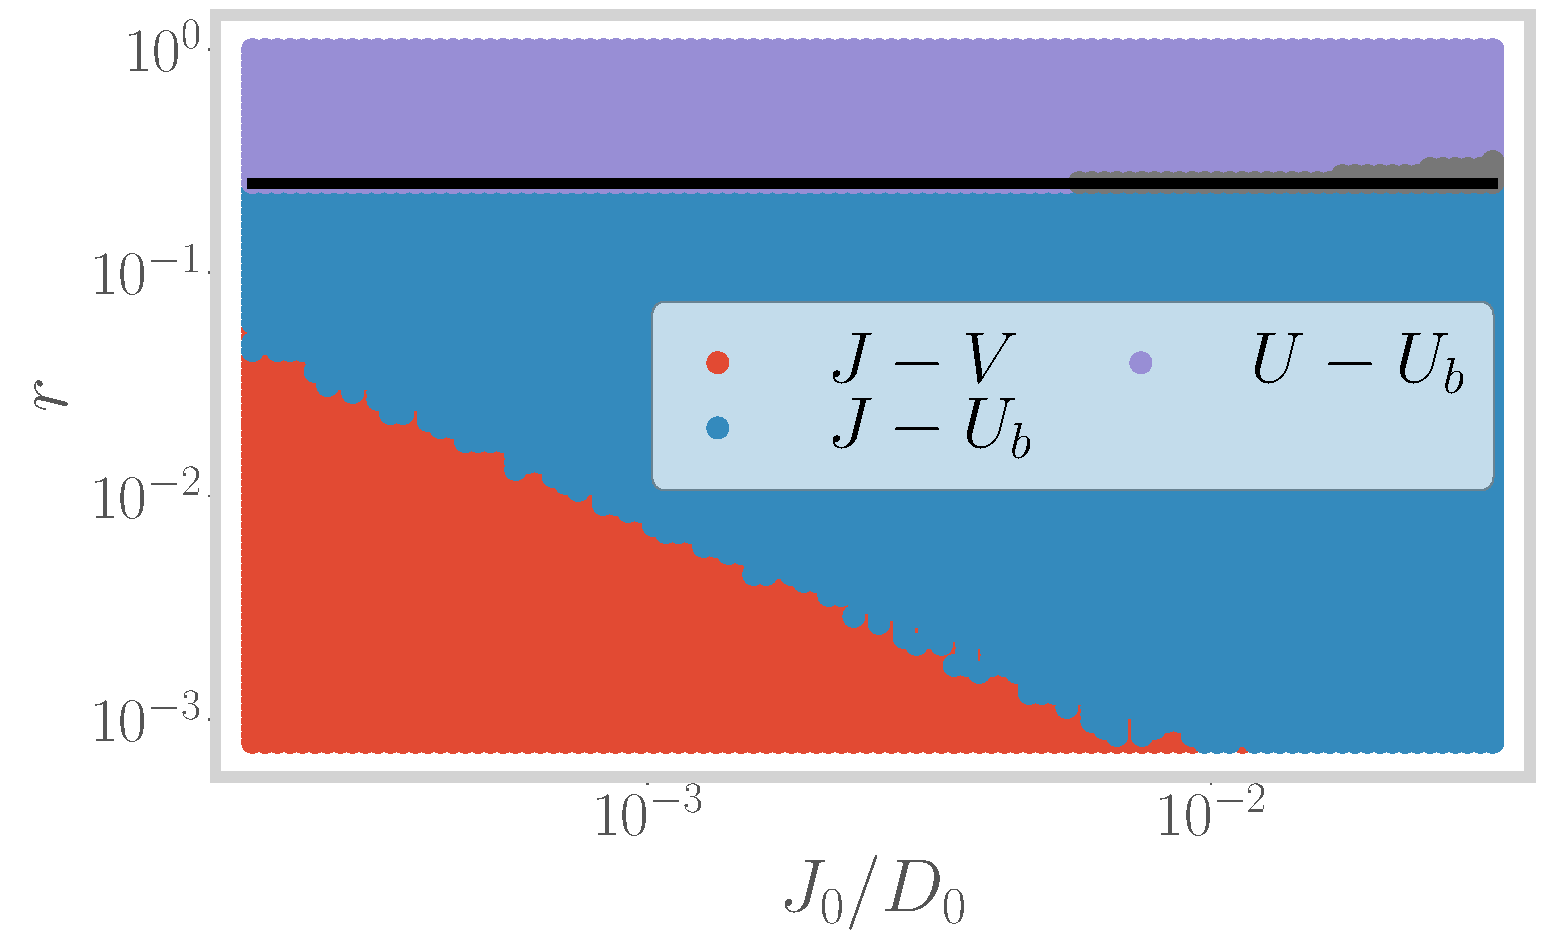
\includegraphics[width=0.48\textwidth]{phase-map-MIT.pdf}
% 	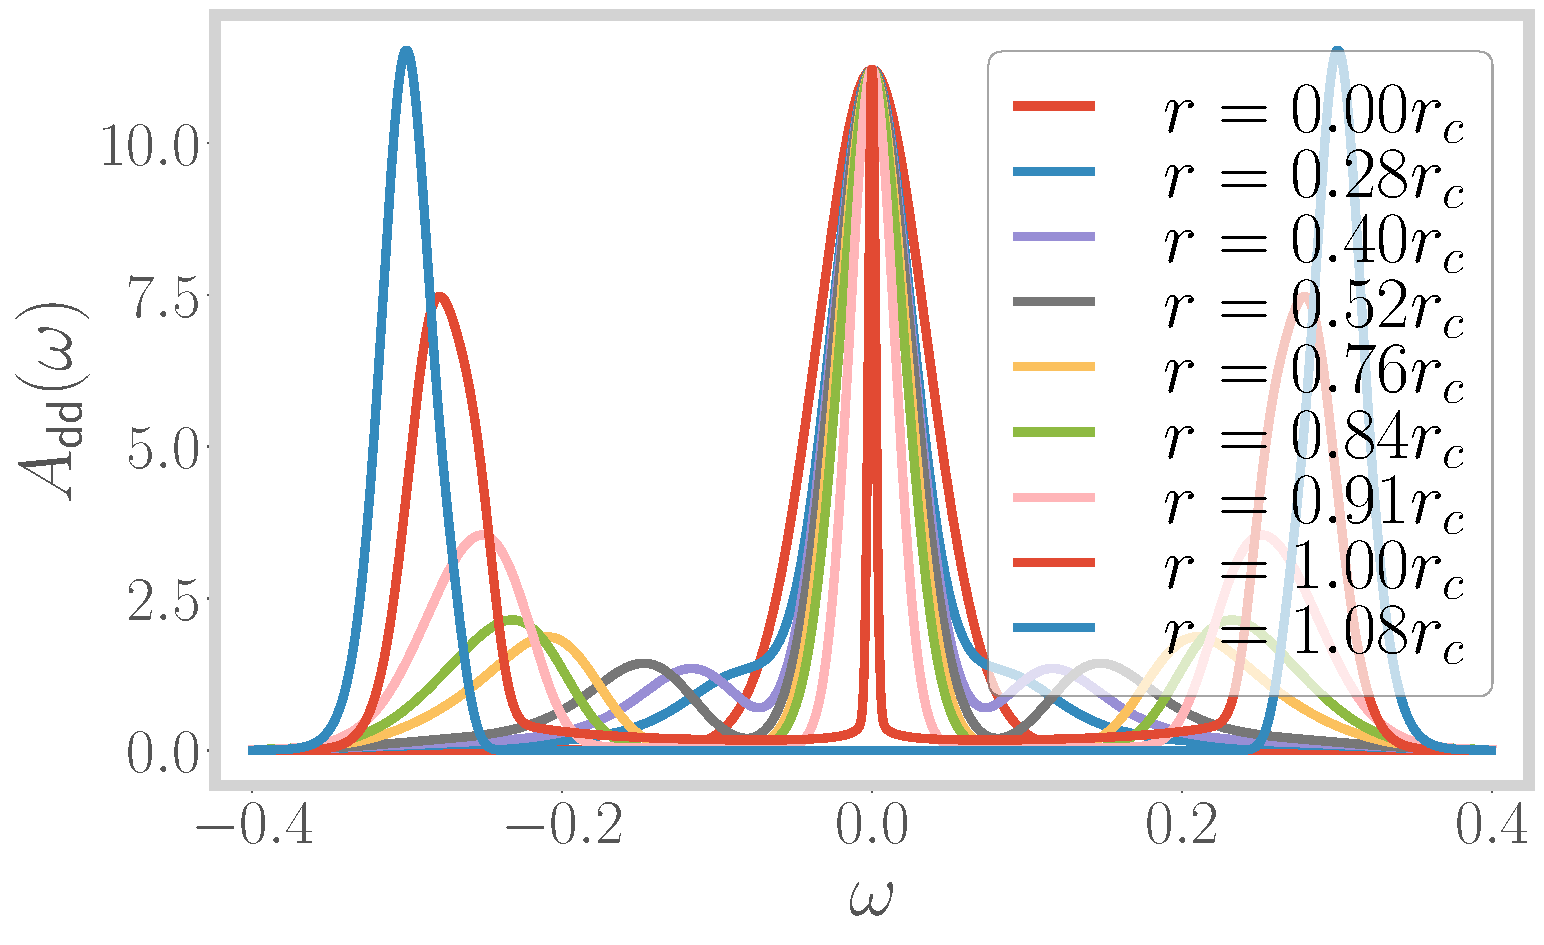
\includegraphics[width=0.48\textwidth]{spectral-function_dd.pdf}
% 	\caption{{\it Left:} Phase diagram of the extended SIAM auxiliary model. As the parameter \(r\) is tuned through 0.25, the metallic blue phase changes into the insulating violet phase. {\it Right:} Local spectral function of the auxiliary model. It shows a hard gap for \(r/r_c > 1\).}
% 	\label{spec_func_mit}
% \end{figure}
%
% The impurity local spectral function \(\mathcal{A}_{dd}(\omega)\) and the impurity-bath real space off-diagonal spectral function \(\mathcal{A}_{dz}(\omega)\) reveal a gap in the spectrum at low \(\omega\) for \(U_b > J/4\). We show the former in fig.~\ref{spec_func_mit}. The gap in the former shows the absence of any gapless excitations that can allow the impurity configuration to fluctuate, while the vanishing of the off-diagonal spectral function shows that this is because the entanglement between the impurity and the bath has been quenched. 
%
% In Fig.~\ref{spin-charge-correlations}, we show the behaviour of the spin-flip and charge isospin-flip correlations between two neighbouring real space sites, as well as the mutual real space entanglement and mutual information. Both show a sharp fall on crossing the transition, demonstrating the destruction of the Kondo cloud and the stabilisation of the local moment on the impurity. Importantly, they charge correlations show a rise very close to the transition (can be seen as a single elevated blue point near \(r = 0.25\) in the left panel of Fig.~\ref{spin-charge-correlations}); this indicates that the transition is precipitated by the growth of pairing correlations.
%
% \begin{figure}[!htb]
% \centering
% 	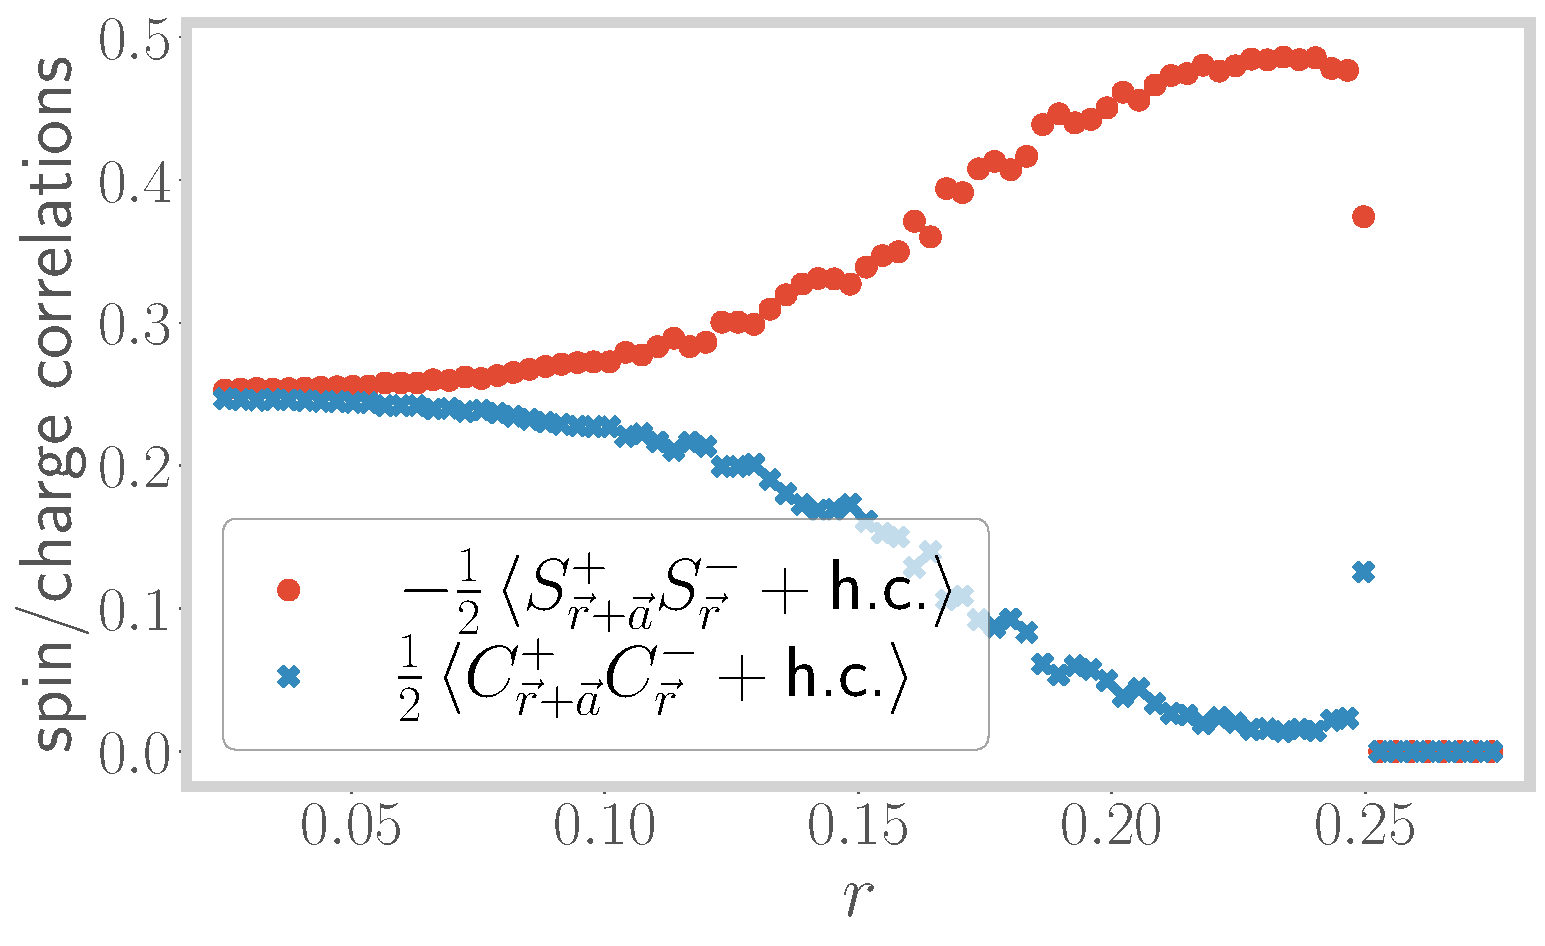
\includegraphics[width=0.48\textwidth]{spin-charge-corr-full.pdf}
% 	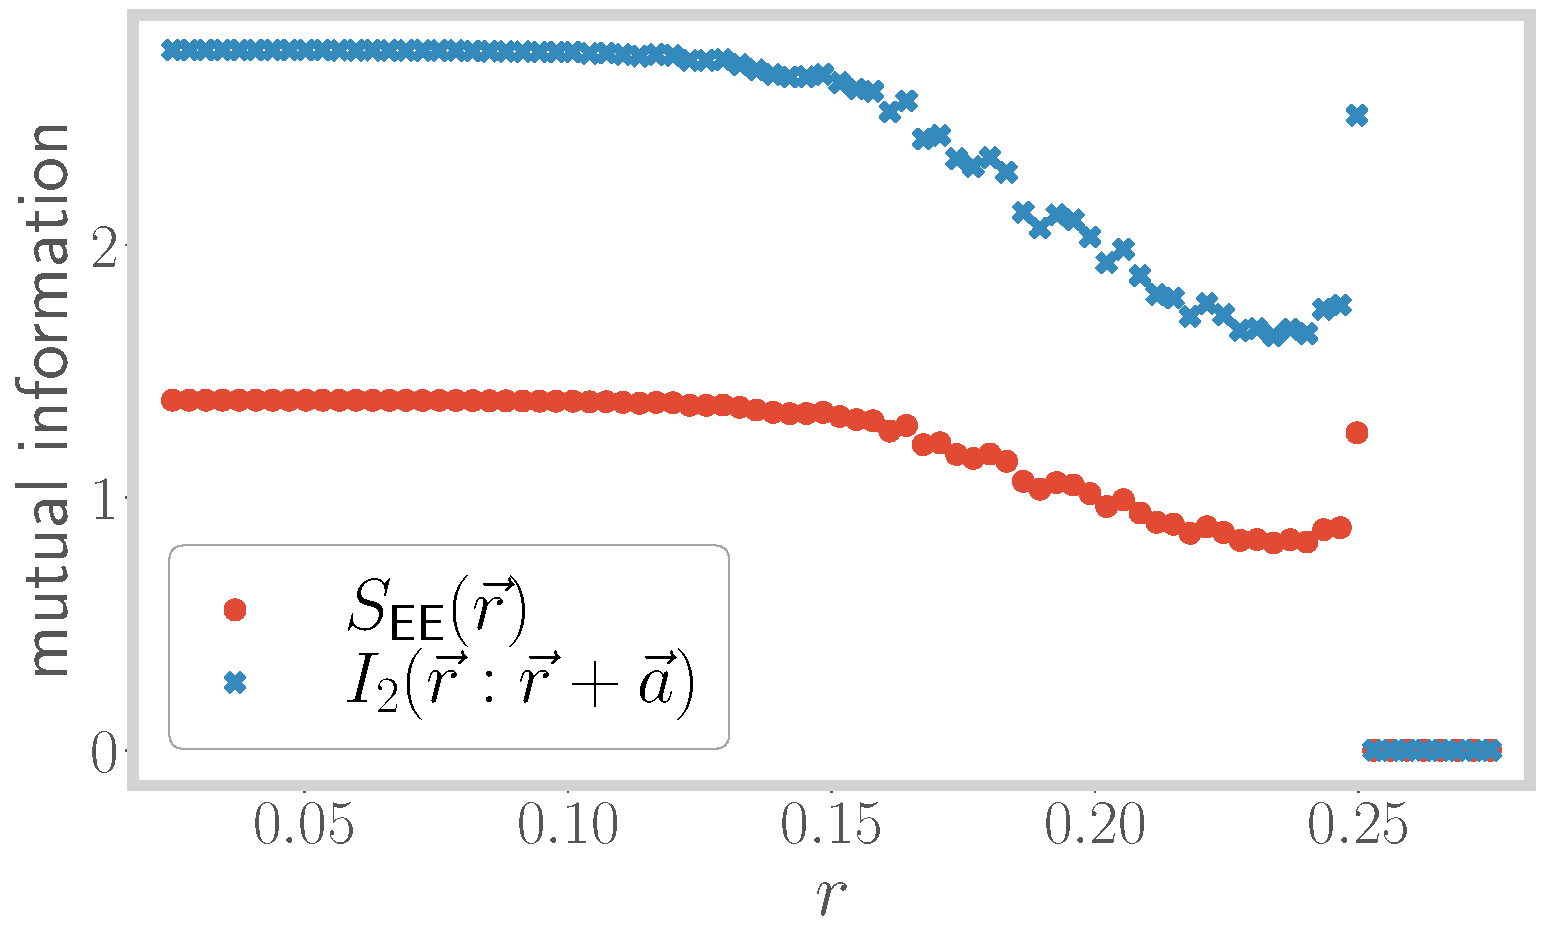
\includegraphics[width=0.48\textwidth]{impEE-mutinfo-d0.pdf}
% 	\caption{{\it Left}: Spin-flip correlations(red) and charge-flip correlations(blue) in real space. The former increases as the system moves into the Kondo regime, and then vanishes at the transition. The latter decreases as the charge content is removed from the ground state in the Kondo regime, but shows a sudden increase at the transition. {\it Right}: Real space Entanglement and mutual information. Both vanish in the local moment phase.}
% 	\label{spin-charge-correlations}
% \end{figure}

\subsection{Value of the critical paramter for the bulk model}
Using the mappings between the auxiliary model parameters and the bulk parameters (eq.~\ref{couplingsMappings}), one can define a critical value \(r^{*}\) of the ratio \(r = U_{H-H}/J_{H-H}\) at the critical points \(-U_b/J=1/4\) \textit{for a given and fixed value of \(U\)}. We will now argue that this critical point describes a metal-insulator transition. For \(r < r^{*}\), the well-defined low-\(\omega\) central peak in the impurity spectral function, as well as the large mutual and information correlations, in the ground state, among the members of the Kondo cloud or between the impurity and the zeroth site show that the impurity and the bath are very strongly entangled. This means that both the local and the nearest-neighbour Greens functions have poles at low\(-\omega\) and support the propagation of electrons through gapless excitations. Since the spectral function is also very simply related to that of the auxiliary model, the former also shows the same zero-energy resonance. 

On the other side \(r > r^{*}\) of the critical point, we know that the impurity gets decoupled from the bath, leading to the transformation of poles into zeros in the Greens functions. This is demonstrated through the gapping of the impurity spectral function in fig.~\ref{spec_func_mit}, and it describes an insulating phase where the electrons get "jammed" in the local states. By the same argument as above, the bulk spectral function also sees a gap in this phase when the impurity spectral function is gapped.

Finally, using relations \eqref{couplingsMappings} between the auxiliary model couplings and the bulk parameters, we can offer a functional form for the critical value of the parameter $r^{*} = U_{H-H}^{*}/J_{H-H}^{*}$. Using \(U_{H-H}^{*} = U^* + U_b\) and \(J_{H-H}^{*} = 2J^*\) (following \eqref{couplingsMappings}), we get
\begin{equation}\begin{aligned}
	r^{*} &=& \frac{1}{2}\left(\frac{U^{*}}{J^{*}} + \frac{U_b}{J^*}\right)
\end{aligned}\end{equation}
where $U^{*}$ and $J^{*}$ are the values of the on-site and Kondo couplings of the auxiliary model at the auxiliary model (i.e., the extended SIAM with a correlated bath) at the transition between the Kondo screened and the local moment phases. By using the auxiliary model criticality condition \(-4U_b = J^*\), the bulk criticality parameter \(r^*\) takes the form
\begin{equation}\begin{aligned}
	r^{*} &=& \frac{1}{2}\left(\frac{U^{*}}{J^{*}} - \frac{1}{4}\right)
\end{aligned}\end{equation}
Parametrising the bath correlation coupling as $U_{b}=-\frac{U}{10}$, we obtain $U^{*}/J^{*}=5/2$, and $r^{*} = 9/8$ for the 2D square lattice Hubbard-Heisenberg model. The reduction in the value of \(r\) from \(2.5\) in the auxiliary model to \(~1.1\) in the bulk model can be attributed to (i) the reduction in the effective bulk repulsion \(U\) due to the competition coming from the attractive \(U_b\), and (ii) increased hybdridisation through \(J\) due to the presence of multiple auxiliary models that connect two lattice sites.


\section{Emergence of effectively pseudogapped Anderson model at the MIT}
%\begin{itemize}
%\item 
We begin by recalling that the RG equation (in the weak coupling limit) of the \(J-U_b\) model that emerges in the Kondo limit of the eSIAM is similar to that of the pseudogapped Anderson model~\cite{fritzvojta2004} that has a bath density of states of the form \(\rho\sim |\omega|^\alpha\). If we define the dimensionless Kondo coupling \(g = \rho J\) and the dimensionless bath coupling \(u = \rho U_b\), the RG equation for \(g\),
\begin{equation}\begin{aligned}
	\Delta g \simeq g^2 + 4gu~,
\end{aligned}\end{equation}
can be mapped to the corresponding RG equation for the pseudogapped Kondo model,
\begin{equation}\begin{aligned}
	\Delta g = g^2 - \alpha g~,
\end{aligned}\end{equation}
with the identification \(\alpha = -4u = -4\rho U_b\). Specifically, this corresponds to a Kondo model that is coupled to a conduction bath with a single-particle density of states that is vanishing (pseudogapped): $\rho\sim |\omega|^{\alpha}$~.
\par
Now, following the work by Si and Kotliar~\cite{kotliarsi_1993}, the impurity self-energy of the \(J-U_b\) model takes the form
	\begin{equation}\begin{aligned}
		\Sigma_{dd} \sim |\omega|^{\gamma_{dd}}~,
	\end{aligned}\end{equation}
	where the exponent \(\gamma_{dd}\) can be written in terms of the phase shifts (at the RG fixed point) \(\delta^*_\text{sp}\) and \(\delta^*_\text{ch}\) suffered by the conduction electrons due to the potentials \(J\) and \(U_b\) respectively in the Hamiltonian:
	\begin{equation}\begin{aligned}
		\gamma_{dd} = \frac{5}{4} - \left[ \frac{1}{\pi}\left( \delta^*_\text{sp} + \delta^*_\text{ch} \right) - \frac{1}{2}  \right]^2 - \left( \frac{\delta^*_\text{ch}}{\pi} \right)^2~.
	\end{aligned}\end{equation}
	The phase shifts are given by \(\delta^*_\text{sp}=\arctan\left( \pi g/2 \right) \) and \(\delta^*_\text{ch}=\arctan\left( \pi u/2 \right) \). In the small coupling limit, these can be approximated as \(\delta^*_\text{sp}=\pi g/2\) and \(\delta^*_\text{ch}=\pi u/2\).
\par 
We now focus on the quantum critical point \(g = -4u\) of our model. At this point, the phase shifts get related to each other: \(\delta^*_\text{sp} = -4\delta^*_\text{ch}\), so that the exponent of the self-energy takes the form
	\begin{equation}\begin{aligned}
		\gamma_{dd} \simeq 1 - \frac{3}{\pi}\delta^*_\text{ch} = 1 + \frac{3}{8}\alpha
	\end{aligned}\end{equation}
	where we have used the fact that for our model, the effective pseudogap parameter \(\alpha\) is set to \(-4u\). The local self-energy then vanishes as
	\begin{equation}\begin{aligned}
		\Sigma_{dd} \sim |\omega|^{\gamma_{dd}} = |\omega|^{1 + \frac{3}{8}\alpha}
	\end{aligned}\end{equation}
The power-law exponent $\gamma_{dd}=1 + \frac{3}{8}\alpha$ lies in the following range: $1\leq \gamma_{dd} \leq 2$. This can be compared with the expression \(\sim|\omega|^{2-3\alpha}\) of the impurity self-energy obtained in ref.~\cite{fritzvojta2004} where the power law exponent ranges between $1/2$ and $2$. In a similar manner, the self-energy \(\Sigma_{dz}\) for scattering processes that connect the impurity site and the bath zeroth site can also be obtained. The exponent \(\gamma_{dz}\) for this self-energy is given by \(\gamma_{dz} = 2 - 2\gamma_{dd}\), so that this non-local self-energy diverges as
\begin{equation}\begin{aligned}\label{selfenergydivergence}
	\Sigma_{dz} \sim |\omega|^{- \frac{3}{4}\alpha}~.
\end{aligned}\end{equation}

We will now relate the auxiliary model self-energies \(\Sigma_{dd}\) and \(\Sigma_{dz}\) with their bulk (or lattice) model counterparts using the lattice Dyson equation. We consider self-energy matrices \(\Sigma\) and \(\Sigma_\text{aux}\) constructed out of real-space self-energies:
\begin{equation}\begin{aligned}
	\Sigma(\omega) = \begin{bmatrix} \Sigma_\text{loc}(\omega) && \Sigma_\text{near-n}(\omega) \\ \Sigma_\text{near-n}(\omega) && \Sigma_\text{loc}(\omega)\end{bmatrix} ,\quad \Sigma_\text{aux}(\omega) = \begin{bmatrix} \Sigma_{dd}(\omega) && \Sigma_{dz}(\omega) \\ \Sigma_{dz}(\omega) && \Sigma_{dd}(\omega)\end{bmatrix}~,
\end{aligned}\end{equation}
where \(\Sigma_\text{loc}\) is the real-space local self-energy and \(\Sigma_\text{near-n}\) is the self-energy for nearest-neighbour scattering processes. Using Dyson's equation, we can write
\begin{equation}\begin{aligned}
	\begin{bmatrix} \Sigma_\text{loc}(\omega) && \Sigma_\text{near-n}(\omega) \\ \Sigma_\text{near-n}(\omega) && \Sigma_\text{loc}(\omega)\end{bmatrix} = \begin{bmatrix} G^{(0)}_\text{loc}(\omega) && G^{(0)}_\text{near-n}(\omega) \\ G^{(0)}_\text{near-n}(\omega) && G^{(0)}_\text{loc}(\omega)\end{bmatrix}^{-1} - \begin{bmatrix} G_\text{loc}(\omega) && G_\text{near-n}(\omega) \\ G_\text{near-n}(\omega) && G_\text{loc}(\omega)\end{bmatrix}^{-1}~,
\end{aligned}\end{equation}
and
\begin{equation}\begin{aligned}
	\begin{bmatrix} \Sigma_{dd}(\omega) && \Sigma_{dz}(\omega) \\ \Sigma_{dz}(\omega) && \Sigma_{dd}(\omega)\end{bmatrix} = \begin{bmatrix} \mathcal{G}^{(0)}_{dd}(\omega) && \mathcal{G}^{(0)}_{dz}(\omega) \\ \mathcal{G}^{(0)}_{dz}(\omega) && \mathcal{G}^{(0)}_{dd}(\omega)\end{bmatrix}^{-1} - \begin{bmatrix} \mathcal{G}_{dd}(\omega) && \mathcal{G}_{dz}(\omega) \\ \mathcal{G}_{dz}(\omega) && \mathcal{G}_{dd}(\omega)\end{bmatrix}^{-1}~,
\end{aligned}\end{equation}
where the superscript \((0)\) indicates that the corresponding quantity has to be calculated from the non-interacting model. We now evaluate the second inverse matrix in each of the two equations, and expression the lattice Greens functions in terms of the auxiliary mode Greens functions (using eqs.~\ref{greens_func_relation} and \ref{greens_func_relation_near}). We get
\begin{equation}\begin{aligned}
	\begin{bmatrix} \Sigma_{dd}(\omega) && \Sigma_{dz}(\omega) \\ \Sigma_{dz}(\omega) && \Sigma_{dd}(\omega)\end{bmatrix} &= 1/\mathcal{G}^{(0)} - \frac{1}{\mathcal{G}_{dd}^2 - \mathcal{G}_{dz}^2}\begin{bmatrix} \mathcal{G}_{dd} && -\mathcal{G}_{dz} \\ -\mathcal{G}_{dz} && \mathcal{G}_{dd}\end{bmatrix}~,\\
	\begin{bmatrix} \Sigma_\text{loc}(\omega) && \Sigma_\text{near-n}(\omega) \\ \Sigma_\text{near-n}(\omega) && \Sigma_\text{loc}(\omega)\end{bmatrix} &= 1/G^{(0)} - \frac{\lambda_{\vec k_0}^2}{\mathcal{G}_{dd}^2 - \mathcal{G}_{dz}^2 / \mathcal{Z}^2}\begin{bmatrix} \mathcal{G}_{dd} && -\frac{1}{\mathcal{Z}}\mathcal{G}_{dz} \\ -\frac{1}{\mathcal{Z}}\mathcal{G}_{dz} && \mathcal{G}_{dd}\end{bmatrix}~.
\end{aligned}\end{equation}
This allows us to write down expressions for the off-diagonal self-energies, in terms of Greens functions, without evaluating the non-singular contribution coming from the non-interacting matrix:
\begin{equation}\begin{aligned}
	\Sigma_{dz} = \left(1/\mathcal{G}^{(0)}\right)_{dz} + \frac{1}{\mathcal{G}_{dd}^2 - \mathcal{G}_{dz}^2} \mathcal{G}_{dz},\quad \Sigma_\text{near-n} = \left(1/G^{(0)}\right)_\text{near-n} + \frac{\lambda_{\vec k_0}^2}{\mathcal{Z}}\frac{1}{\mathcal{G}_{dd}^2 - \mathcal{G}_{dz}^2 / \mathcal{Z}^2} \mathcal{G}_{dz}
\end{aligned}\end{equation}
The divergence of \(\Sigma_{dz}\) shown in eq.~\ref{selfenergydivergence} as \(\omega \to 0\) has to arise from the second term in the expression for \(\Sigma_{dz}\) above as it contains the effects of inter-particle correlations.
%, because the non-interacting Greens function has well-defined poles which kill the first term. 
Importantly, we note that the second term in the expression for \(\Sigma_\text{near-n}\) is very similar to the diverging term in \(\Sigma_{dz}\), differing only through the presence of some finite (i.e., non-divergent) non-zero factors of \(\lambda_{\vec k_0}^2\) and \(\mathcal{Z}\). We therefore conclude that the non-local self-energy of the lattice model $\Sigma_\text{near-n}$ contains the same power-law divergence  as $\Sigma_{dz}$ upon taking the limit $\omega\to 0$:
\begin{equation}\begin{aligned}
	\Sigma_\text{near-n}\left( \omega \right) \sim \omega^{-3\alpha/4}~.
\end{aligned}\end{equation}
By a similar argument, the local self-energy is found to vanish as \(\omega \to 0\). We have seen above that we can approximate the \(k-\)space self-energy in terms of these two real-space self-energies (eq.\eqref{selfenergy1}):
\begin{equation}\begin{aligned}
	\Sigma(\vec k, \omega) \simeq \Sigma_\text{loc}(\omega) + \tilde{\Sigma}(\vec k, \omega)~,~~\textrm{where}~\tilde{\Sigma}(\vec k, \omega)=\xi_{\vec k}\Sigma_\text{near-n}~,
\end{aligned}\end{equation}
and $\xi_{\vec{k}}$ is the electronic lattice dispersion (in units of the hopping amplitude $t$). It is clear from the expression that the divergent $\Sigma_\text{near-n}$ does not affect the single-particle self-energy $\Sigma(\vec k,\omega)$ at the Fermi surface, i.e., for $\xi_{\vec{k}}= 0$, but $\Sigma(\vec k,\omega)$ diverges everywhere else in the Brillouin zone. This corresponds to a gapless non-Fermi liquid metal present at the QCP, corresponding to a system with Landau quasiparticle poles precisely on the Fermi surface but which are destroyed everywhere else.

Now, following the arguments laid out in Ref.\cite{sujan2023}, the single-particle spectral function $A(\omega,\vec{k})$ will vanish (i.e., be pseudogapped) for excitations away from a critical Fermi surface~(see Chapter 8 of Ref.\cite{carr2010})
\begin{equation}
A(\vec{k},\omega) \sim |\omega|^{\frac{3}{4}\alpha}~.
\end{equation}	
This corresponds to the vanishing of the residue of the Landau quasiparticle precisely at the metal-insulator transition, and the emergence of a gapless non-Fermi liquid ``local quantum critical" metal~\cite{Si2001}. Further, the fact that the single-particle self-energy $\Sigma(\vec k, \omega)$ vanishes precisely at the Fermi surface signals the fact that the Luttinger's count for states on the Fermi surface is preserved and identical to that in the Fermi liquid phase. 



\section{Topological nature of the transition}
Since the impurity charge hybridising with the bath contributes to the total Luttinger volume of the system~\cite{martin1982fermi}, decoupling of the impurity from the conduction bath leads to a difference in the value of the Luttinger volume between the local moment (LM) and the strong-coupling (SC) fixed points. If we define \(\mathcal{N}_L\) as the Luttinger volume with the spin-degeneracy accounted for, we can write
\begin{equation}\begin{aligned}
	\label{lutt_change}
	\mathcal{N}_L^\text{lm} - \mathcal{N}_L^\text{sc} = 1
\end{aligned}\end{equation}
where \(\mathcal{N}_L^\text{lm},\mathcal{N}_L^\text{sc}\) are the Luttinger volumes at the local moment and strong-coupling fixed points respectively. This equation expresses the fact that the Luttinger volume of the bath increases by \(1\) when the system is tuned from LM to SC, and this happens because the single-particle impurity excitation in the lower-Hubbard at the atomic limit gets transferred to the bath Greens function in the process. The quantity which tracks this transfer is therefore \(\mathcal{N}_\text{imp}\), the number of poles minus the number of zeros in the impurity Greens function at and below the Fermi surface:
\begin{equation}\begin{aligned}
	\label{imp_count_def}
	\mathcal{N}_\text{imp} = \begin{cases}
		1 & \text{ at LM}\\
		0 & \text{ at SC}
	\end{cases}\implies \Delta \mathcal{N}_\text{imp} = 1
\end{aligned}\end{equation}
The Luttinger volume \(\mathcal{N}_L\) is related to this impurity count by the equation
\begin{equation}\begin{aligned}
	\mathcal{N}_L = \mathcal{N} - \mathcal{N}_\text{imp}
\end{aligned}\end{equation}
where \(\mathcal{N}\) is the total number of electrons in the system, accounting for the spin degeneracy. If we keep this total number fixed (isolated system), the changes in the impurity count and Luttinger volume become constrained: 
\begin{equation}\begin{aligned}
	\Delta \mathcal{N}_L = - \Delta \mathcal{N}_\text{imp}~.
\end{aligned}\end{equation}
Eq.~\ref{imp_count_def} then readily implies eq.~\ref{lutt_change}.

In order to connect this impurity topological change with the bulk model, we write the total number of particles in the bulk system in the following manner:
\begin{equation}\begin{aligned}
	\mathcal{N} = \mathcal{N}_\text{loc} + \mathcal{N}_\text{deloc}
\end{aligned}\end{equation}
\(\mathcal{N}_\text{loc}\) is the number of real poles minus the number of zeros of the local Greens function. \(\mathcal{N}_\text{deloc}\) is the number of real poles minus the number of zeros of the \(k-\)space Greens functions. The former (latter) contributes only in the insulating (metallic) phase, because in the metallic (insulating) phase, the local (\(k-\)space) Greens function develop imaginary self-energy and the real poles in these Greens functions get replaced by imaginary poles. Together, these two terms accurately count the total number of particles in both these phases. These two terms are defined as
\begin{equation}\begin{aligned}
	\mathcal{N}_\text{loc} = \sum_i \mathcal{N}_i = \oint \frac{dz}{2\pi i}n_F(z) \text{Tr}\left[G_i(z)\right], ~ ~ ~\mathcal{N}_\text{deloc} = \sum_k \mathcal{N}_k = \oint \frac{dz}{2\pi i}n_F(z) \text{Tr}\left[G_k(z)\right] = \mathcal{N}_L
\end{aligned}\end{equation}
\(G_i(z)\) is the local Greens function at site \(i\) of the bulk model, and \(G_k(z)\) is the \(k-\)space Greens function in the bulk model. \(N_\text{deloc}\) is just the Luttinger volume \(\mathcal{N}_L\) of the bulk system. With this, the total number of particles in the bulk can be expressed as
\begin{equation}\begin{aligned}
	\label{bulk_total}
	\mathcal{N} = \sum_i \mathcal{N}_i + \mathcal{N}_\text{L}
\end{aligned}\end{equation}
From eq.~\ref{greens_func_relation}, we know that the bulk local Greens function is proportional to that of the auxiliary model, and that gives \(\sum_i \mathcal{N}_i = \mathcal{N}_\text{imp}\sum_i = \mathcal{N} \mathcal{N}_\text{imp}\). There we used the fact that for a half-filled system, the total number of sites is equal to the total number of particles in the system. Substituting this into eq.~\ref{bulk_total} and again using \(\Delta \mathcal{N} = 0\) gives
\begin{equation}\begin{aligned}
	\mathcal{N} = \mathcal{N} \mathcal{N}_\text{imp} + \mathcal{N}_\text{L} \implies \Delta \mathcal{N}_\text{L} = - \mathcal{N} \Delta \mathcal{N}_\text{imp}
\end{aligned}\end{equation}
We already know that \(\Delta \mathcal{N}_\text{imp}=1\) across the transition, so we get
\begin{equation}\begin{aligned}
	\mathcal{N}_L^\text{metal} - \mathcal{N}_L^\text{insulator} = \mathcal{N}\left(\mathcal{N}_\text{imp}^\text{sc} - \mathcal{N}_\text{imp}^\text{lm}\right) = \mathcal{N}
\end{aligned}\end{equation}
The metal-insulator transition is therefore characterised by a change in the topological quantity \(\mathcal{N}_L\). The topological nature arises from the fact that it can be expressed in terms of winding numbers related to the corresponding Greens functions. \(\mathcal{N}_\text{imp}\), which derives from the impurity Greens function \(G_d\), is related to the winding numbers of the curves \(\text{Det}[G_d^{-1}(\Gamma^<)]\) and \(\text{Det}[G_d^{-1}(\Gamma^0)]\). The winding number is simply the number of times this function encircles the origin when traced on the curves \(\Gamma^<\) and \(\Gamma^0\) that enclose all poles inside and on the Fermi surface respectively. An example of such a winding number is shown in fig.~\ref{imp_winding}.
\begin{figure}[!htb]
	\centering
	\includegraphics[width=0.4\textwidth]{windingNumbers.pdf}
	\caption{The green lines describe the winding number related to the impurity Greens function, while the blue lines do it for the bath. At the local moment fixed point \(V=0\), the impurity has a winding number of 1 because the curve encircles the origin once. At the strong-coupling fixed point, this winding number becomes zero, indicated by the fact that the curve does not encircle the origin even once. The reduction in the winding number on the part of the impurity is directly linked to the increase in the winding number of the bath - it encircles the origin once at the local moment fixed point but twice at strong-coupling.}
	\label{imp_winding}
\end{figure}


\clearpage
\section*{Appendices}
\appendix
\section{Effective action for the Hubbard-Heisenberg model and the eSIAM}
In order to better understand the similarities and differences between the tiling approach outlined here and the approach adopted in dynamical mean-field approximations, we compute the effective action for the local impurity as well as the impurity-zeroth site system, in both the auxiliary and bulk models. This will be done in the limit of infinite coordination number, in order to create a tractable effective theory.

\subsection{Local theory for the Hubbard-Heisenberg model}
We will first work with the Hubbard-Heisenberg model. Let us recall that within the eSIAM, most of the dynamics is governed by the physics of the impurity site and the bath site coupled to the impurity. Accordingly, we will first obtain an effective action within the Hubbard-Heisenberg model for the small system consisting of a local site and all its nearest-neighbours. 

We choose a certain local site that we call \(0\), whose nearest-neighbours will be denoted as \(\left\{ {\bar 0} \right\} \). The action for the full Hubbard-Heisenberg model can be formally separated into three parts:
\begin{equation}\begin{aligned}
S_\text{H-H} = S_{0,{\bar 0}} + S^{(0,{\bar 0})} + S_\text{int}~,
\end{aligned}\end{equation}
where \(S_{0,{\bar 0}}\) represents the part of the action that involves only the sites \(0\) and $\left\{ {\bar 0} \right\}$, \(S^{(0,{\bar 0})}\) represents the part that has all the sites apart from \(0\) and \(\left\{ {\bar 0} \right\} \), while \(S_\text{int}\) contains all terms that connect these two parts. These three parts have the forms
\begin{equation}\begin{aligned}
S_{0,{\bar 0}} = \sum_{i=0,{\bar 0}}\sum_\sigma \int_0^\beta\mathrm{d\tau}~c^\dagger_{i\sigma}(\tau)\partial_\tau c_{i\sigma}(\tau)  - t\sum_{{\bar 0},\sigma}\int_0^\beta\mathrm{d\tau}~\left[c^\dagger_{0\sigma}(\tau)c_{{\bar 0}\sigma}(\tau) + \text{h.c.}\right] \\
- \frac{U}{2}\sum_{i=0,{\bar 0}}\int_0^\beta\mathrm{d\tau}~\left(n_{i \uparrow}(\tau) - n_{i \downarrow}(\tau)\right)^2 + J\sum_{{\bar 0}}\int_0^\beta\mathrm{d\tau} \vec{S}_0(\tau)\cdot\vec{S}_{{\bar 0}}(\tau)~,
\end{aligned}\end{equation}
\begin{equation}\begin{aligned}
S^{(0,{\bar 0})} = \sum_{j\neq(0,{\bar 0})}\sum_\sigma \int_0^\beta\mathrm{d\tau}~c^\dagger_{j\sigma}(\tau)\partial_\tau c_{j\sigma}(\tau)  - t\sum_{\left<j,l\right>\neq (0,{\bar 0}),\sigma}\int_0^\beta\mathrm{d\tau}~\left[c^\dagger_{j\sigma}(\tau)c_{l\sigma}(\tau) + \text{h.c.}\right] \\
- \frac{U}{2}\sum_{j\neq(0,{\bar 0})}\int_0^\beta\mathrm{d\tau}~\left(n_{j\uparrow}(\tau) - n_{j\downarrow}(\tau)\right)^2 + J\sum_{\left<j,l\right>\neq(0,{\bar 0})}\int_0^\beta\mathrm{d\tau} \vec{S}_l(\tau)\cdot\vec{S}_j(\tau)~,
\end{aligned}\end{equation}
\begin{equation}\begin{aligned}
S_\text{int} = -t\sum_{i \in {\bar 0}}\sum_{j \in \text{NN of}~i}\sum_\sigma \int_0^\beta\mathrm{d\tau}~\left(c^\dagger_{i\sigma}(\tau) c_{j\sigma}(\tau) + \text{h.c.}\right) + J\sum_{i \in {\bar 0}}\sum_{j \in \text{NN of}~i}\int_0^\beta\mathrm{d\tau}\vec{S}_i(\tau)\cdot\vec{S}_j(\tau) = S_\text{int}^\text{hop} + S_\text{int}^\text{spin} 
\end{aligned}\end{equation}

In order to obtain an effective theory \(S^{0,{\bar 0}}_\text{eff}\) purely for the local system \((0,{\bar 0})\), we need to trace over all the other degrees of freedom. This partial trace will be carried out over the states of the so-called ``cavity" system \(S^{(0,{\bar 0})}\). The effective action can be constructed by tracing over scattering processes of all orders that leave the final action diagonal in the system \((0,{\bar 0})\). The formal expression can be written as
\begin{equation}\begin{aligned}
	S^{0,{\bar 0}}_\text{eff} = S_{0,{\bar 0}} + \sum_{n=1}^\infty \braket{\left(S_\text{int}^\text{hop}\right)^{2n}}_{(0,{\bar 0})} + \sum_{n=1}^\infty \braket{\left(S_\text{int}^\text{spin}\right)^{2n}}_{(0,{\bar 0})}
\end{aligned}\end{equation}
where, as mentioned before, the average is carried out in the cavity system \(S^{(0,{\bar 0})}\). Each hopping term in the expansion is of the form
\begin{equation}\begin{aligned}
	\left(S_\text{int}^\text{hop}\right)^{2n} =& t^{2n}\sum_\sigma\sum_{(i_1, i_1^\prime)\ldots, (i_n, i_n^\prime)} ~\sum_{(j_1, j_1^\prime)\ldots, (j_n, j_n^\prime)} \int_0^\beta d\tau_{1}\ldots d\tau_{n}d\tau_{1}^\prime\ldots d\tau_{j_n}^\prime\\
			   &c^\dagger_{i_1\sigma}(\tau_{i_1})c^\dagger_{i_2\sigma}(\tau_{2})\ldots c^\dagger_{i_n\sigma}(\tau_{n}) c_{i_1^\prime\sigma}(\tau_{1}^\prime)c_{i_2^\prime\sigma}(\tau_{2}^\prime)\ldots c_{i_n^\prime\sigma}(\tau_{n}^\prime)\left<c_{j_1\sigma}(\tau_{1})c_{j_2\sigma}(\tau_{2})\ldots c_{j_n\sigma} ~ c^\dagger_{j_1^\prime\sigma}(\tau_{1}^\prime)\ldots c^\dagger_{j_n^\prime\sigma}(\tau_{n}^\prime) \right>_{(0,{\bar 0})}\\
	=& t^{2n}\sum_\sigma\sum_{(i_1, i_1^\prime)\ldots, (i_n, i_n^\prime)} ~\sum_{(j_1, j_1^\prime)\ldots, (j_n, j_n^\prime)} \int_0^\beta d\tau_{1}\ldots d\tau_{j_n}^\prime c^\dagger_{i_1\sigma}(\tau_{i_1})\ldots c^\dagger_{i_n\sigma}(\tau_{n})~c_{i_1^\prime\sigma}(\tau_{1}^\prime)\ldots c_{i_n^\prime\sigma}(\tau_{n}^\prime)\\
	 &G_n^{(0,\bar 0)}\left(\tau_1\ldots \tau_n; \tau_1^\prime\ldots \tau_n^\prime\right)~,
\end{aligned}\end{equation}
where the indices \(i_1\) through \(i_n\) and their primed counterparts run through \(\bar 0\), while \(j_l\) (\(\in \left\{j_1,\ldots,j_n^\prime\right\}\)) runs through the nearest-neighbours of the corresponding \(i_l\) index. The \(n-\)particle Greens function \(G_n^{(0,\bar 0)}\left(\tau_1\ldots \tau_n; \tau_1^\prime\ldots \tau_n^\prime\right)\) for the cavity system is defined in the usual fashion
\begin{equation}\begin{aligned}
	G_n^{(0,\bar 0)}\left(\tau_1\ldots \tau_n; \tau_1^\prime\ldots \tau_n^\prime\right) = \left<c_{j_1\sigma}(\tau_{1})c_{j_2\sigma}(\tau_{2})\ldots c_{j_n\sigma} ~ c^\dagger_{j_1^\prime\sigma}(\tau_{1}^\prime)\ldots c^\dagger_{j_n^\prime\sigma}(\tau_{n}^\prime) \right>_{(0,{\bar 0})} 
\end{aligned}\end{equation}
In the limit of infinite coordination number, only the \(n=1\) term survives:
\begin{equation}\begin{aligned}
	\lim_{\mathcal{Z}\to \infty}\sum_{n=1}^\infty \braket{\left(S_\text{int}^\text{hop}\right)^{2n}}_{(0,{\bar 0})} = t^2\sum_{\sigma}\sum_{i,i^\prime}\int_0^\beta\mathrm{d\tau}\mathrm{d\tau^\prime}c^\dagger_{i\sigma}(\tau)c_{i^\prime\sigma}(\tau^\prime)\sum_{j,j^\prime}G_1^{(0,\bar 0)}\left(j\tau; j^\prime\tau^\prime\right) \\
	= \sum_{\sigma}\sum_{i,i^\prime}\int_0^\beta\mathrm{d\tau}\mathrm{d\tau^\prime}~\Delta_{ii^\prime,\sigma}(\tau - \tau^\prime)c^\dagger_{i\sigma}(\tau)c_{i^\prime\sigma}(\tau^\prime)~,
\end{aligned}\end{equation}
where we have defined the bath hybridisation function \(\Delta_{ii^\prime,\sigma}(\tau - \tau^\prime)\) as
\begin{equation}\begin{aligned}
	\Delta_{ii^\prime,\sigma}(\tau - \tau^\prime) = t^2\sum_{j \in \text{NN of}~i}\sum_{j^\prime \in \text{NN of}~i^\prime}G_1^{(0,\bar 0)}\left(j\sigma\tau; j^\prime\sigma\tau^\prime\right)~.
\end{aligned}\end{equation}

Under similar approximations, the spin term in the action reduces to
\begin{equation}\begin{aligned}
	\lim_{\mathcal{Z}\to \infty}\sum_{n=1}^\infty \braket{\left(S_\text{int}^\text{spin}\right)^{2n}}_{(0,{\bar 0})} = \sum_{i,i^\prime}\int_0^\beta\mathrm{d\tau}\mathrm{d\tau^\prime}~\chi(\tau - \tau^\prime)\vec{S}_{i}(\tau)\cdot\vec{S}_{i^\prime}(\tau^\prime)~,
\end{aligned}\end{equation}
where the susceptibility \(\chi_{ii^\prime}(\tau - \tau^\prime)\) is defined as 
\begin{equation}\begin{aligned}
	\chi_{ii^\prime}(\tau - \tau^\prime) = J^2\sum_{j \in \text{NN of}~i}\sum_{j^\prime \in \text{NN of}~i^\prime}\vec{S}_{j}(\tau)\cdot\vec{S}_{j^\prime}(\tau^\prime)~.
\end{aligned}\end{equation}
The effective action for the \(0,\bar 0\) system, in the limit of large coordination number, simplifies to
\begin{equation}\begin{aligned}
	S^{0,{\bar 0}}_\text{eff} =& \sum_{i=0,{\bar 0}}\sum_\sigma \int_0^\beta\mathrm{d\tau}~c^\dagger_{i\sigma}(\tau)\partial_\tau c_{i\sigma}(\tau)  - t\sum_{{\bar 0},\sigma}\int_0^\beta\mathrm{d\tau}~\left[c^\dagger_{0\sigma}(\tau)c_{{\bar 0}\sigma}(\tau) + \text{h.c.}\right] - \frac{U}{2}\sum_{i=0,{\bar 0}}\int_0^\beta\mathrm{d\tau}~\left(n_{i \uparrow}(\tau) - n_{i \downarrow}(\tau)\right)^2 \\
				   &+ J\sum_{{\bar 0}}\int_0^\beta\mathrm{d\tau} \vec{S}_0(\tau)\cdot\vec{S}_{{\bar 0}}(\tau) + \sum_{i,i^\prime}\int_0^\beta\mathrm{d\tau}\mathrm{d\tau^\prime}~\left[\sum_{\sigma}\Delta_{ii^\prime,\sigma}(\tau - \tau^\prime)c^\dagger_{i\sigma}(\tau)c_{i^\prime\sigma}(\tau^\prime) + \chi_{ii^\prime}(\tau - \tau^\prime)\vec{S}_{i}(\tau)\cdot\vec{S}_{i^\prime}(\tau^\prime)\right]
\end{aligned}\end{equation}

One can also write down an effective action purely for the local site \(0\). The sites \(\bar 0\) will now be a part of the environment action \(S^{(0)}\) instead of the system action, but since the system is thermodynamically large, the cavity action can be assumed to remain the same, such the expectation values are calculated in the same system. As a result, the hybridisation and susceptibility functions remain unchanged. \(S_\text{int}\) is now made of terms that connect \(0\) and \(\bar 0\), so the transformation from \(S^{(0,\bar 0)}\) can be made by replacing the set \(\left\{ j \right\} \) with the set \(\bar 0\), and the set \(\bar 0\) itself will be replaced by the local site \(0\). We quote the final form of the local effective action:
\begin{equation}\begin{aligned}
	S^{0}_\text{eff} =& \sum_\sigma \int_0^\beta\mathrm{d\tau}~c^\dagger_{0\sigma}(\tau)\partial_\tau c_{0\sigma}(\tau) - \frac{U}{2}\int_0^\beta\mathrm{d\tau}~\left(n_{0\uparrow}(\tau) - n_{0\downarrow}(\tau)\right)^2 \\
			  &+ \int_0^\beta\mathrm{d\tau}\mathrm{d\tau^\prime}~\left[\sum_{\sigma}\Delta_{00,\sigma}(\tau - \tau^\prime)c^\dagger_{i\sigma}(\tau)c_{i^\prime\sigma}(\tau^\prime) + \chi_{00}(\tau - \tau^\prime)\vec{S}_{i}(\tau)\cdot\vec{S}_{i^\prime}(\tau^\prime)\right]
\end{aligned}\end{equation}

\subsection{Local theory for the extended SIAM}
The Hamiltonian for the extended SIAM model is shown in eq.~\ref{siam_attr}. We will denote the impurity with the label \(d\) and the bath sites with the label \(c\). Among the bath sites, we will represent the site coupled to the impurity with \(z\). The full action has the form
\begin{equation}\begin{aligned}
	S_\text{ES} = \sum_{d,c}\sum_\sigma \int_0^\beta\mathrm{d\tau}~c^\dagger_{i\sigma}(\tau)\partial_\tau c_{i\sigma}(\tau) - t\sum_{\left<i,j \right> \in c,\sigma}\int_0^\beta\mathrm{d\tau}~\left[c^\dagger_{i\sigma}(\tau)c_{j\sigma}(\tau) + \text{h.c.}\right] - V\sum_{\sigma}\int_0^\beta\mathrm{d\tau}~\left[c^\dagger_{d\sigma}(\tau)c_{z\sigma}(\tau) + \text{h.c.}\right]\\
+ J\int_0^\beta\mathrm{d\tau} \vec{S}_d(\tau)\cdot\vec{S}_{z}(\tau) - \frac{U}{2}\int_0^\beta\mathrm{d\tau}~\left(n_{d\uparrow}(\tau) - n_{d\downarrow}(\tau)\right)^2 - \frac{U_b}{2}\int_0^\beta\mathrm{d\tau}~\left(n_{z\uparrow}(\tau) - n_{z\downarrow}(\tau)\right)^2 ~,
\end{aligned}\end{equation}
As in the Hubbard-Heisenberg model, we first obtain an effective action for the pair of sites \((d,z)\). As in the previous calculation, this will again generate a hybridisation function \(\Delta_{zz,\sigma}\) for the bath site nearest to the zeroth site. No susceptibility will be generated however, because there is no spin-exchange coupling within the bath. The net result is
\begin{equation}\begin{aligned}
	S^{d,z}_\text{eff} =& \sum_{d,c}\sum_\sigma \int_0^\beta\mathrm{d\tau}~c^\dagger_{i\sigma}(\tau)\partial_\tau c_{i\sigma}(\tau) - V\sum_{\sigma}\int_0^\beta\mathrm{d\tau}~\left[c^\dagger_{d\sigma}(\tau)c_{z\sigma}(\tau) + \text{h.c.}\right] + J\int_0^\beta\mathrm{d\tau} \vec{S}_d(\tau)\cdot\vec{S}_{z}(\tau) \\
	&- \frac{U}{2}\int_0^\beta\mathrm{d\tau}~\left(n_{d\uparrow}(\tau) - n_{d\downarrow}(\tau)\right)^2 - \frac{U_b}{2}\int_0^\beta\mathrm{d\tau}~\left(n_{z\uparrow}(\tau) - n_{z\downarrow}(\tau)\right)^2 \\
	&+ \int_0^\beta\mathrm{d\tau}\mathrm{d\tau^\prime}~\sum_{\sigma}\Delta_{zz,\sigma}(\tau - \tau^\prime)c^\dagger_{z\sigma}(\tau)c_{z\sigma}(\tau^\prime)
\end{aligned}\end{equation}
This hybridisation \(\Delta_{zz,\sigma}\) is calculated in the cavity model of the eSIAM, obtained by removing the impurity and the zeroth site from the full model; it is a completely non-interacting system.

One can go one step further and also remove the zeroth site in order to obtain a theory for the impurity site. With this choice, the cavity model now also includes the zeroth site, and hence contains the correlation term associated with \(U_b\). The one-particle connection \(V\) will lead to a modified hybridisation \(\mathcal{F}\) for this effective theory; the Kondo terms will generate a susceptibility. The resultant action is
\begin{equation}\begin{aligned}
	S^{d}_\text{eff} =& \sum_\sigma \int_0^\beta\mathrm{d\tau}~c^\dagger_{d\sigma}(\tau)\partial_\tau c_{d\sigma}(\tau) - \frac{U}{2}\int_0^\beta\mathrm{d\tau}~\left(n_{d\uparrow}(\tau) - n_{d\downarrow}(\tau)\right)^2 \\
			  &+ \int_0^\beta\mathrm{d\tau}\mathrm{d\tau^\prime}~\left[\sum_{\sigma}\mathcal{F}_{\sigma}(\tau - \tau^\prime)c^\dagger_{i\sigma}(\tau)c_{i^\prime\sigma}(\tau^\prime) + \chi_{d}(\tau - \tau^\prime)\vec{S}_{i}(\tau)\cdot\vec{S}_{i^\prime}(\tau^\prime)\right]
\end{aligned}\end{equation}
where \(\mathcal{F}\) is defined in terms of the local correlator of the zeroth site
\begin{equation}\begin{aligned}
	\mathcal{F}_\sigma(\tau - \tau^\prime) = V^2 G_1^{(d)}\left(z\sigma\tau; z\sigma\tau^\prime\right) = V^2 \left<c_{z\sigma}(\tau)c^\dagger_{z\sigma}(\tau^\prime)\right>_{(d)}
\end{aligned}\end{equation}
with the average computed in the interacting cavity model that has the impurity site removed. The interaction arises from the \(U_b-\)term. The susceptibility is also calculated in this interacting cavity model, and follows the same definition as in the bulk model:
\begin{equation}\begin{aligned}
	\chi_{d}(\tau - \tau^\prime) = J^2\vec{S}_{z}(\tau)\cdot\vec{S}_{z}(\tau^\prime)~.
\end{aligned}\end{equation}
\section{Zero temperature Greens function in frequency domain}

\label{appx-spectral-func}

\subsection{Spectral representation of Greens function}
The impurity retarded Green's function is defined as
\begin{equation}\begin{aligned}
	G_{d\sigma}(t) = -i\theta(t) \left<\left\{ \mathcal{O}_{\sigma}(t),\mathcal{O}^\dagger_{\sigma} \right\}  \right>
\end{aligned}\end{equation}
where the average \(\left< \right>\) is over a canonical ensemble at temperature \(T\), and \(\mathcal{O}_\sigma\) is the excitation whose spectral function we are interested in. What follows is a standard calculation where we write the Green's function in the spectral representation. The ensemble average for the operator \(\mathcal{O}_\sigma\) can be written in terms of the exact eigenstates of the Hamiltonian:
\begin{equation}\begin{aligned}
	H \ket{n} &= E_n \ket{n}, \quad\left<\mathcal{O}_\sigma\right> &\equiv \frac{1}{Z}\sum_n \braket{n | \mathcal{O}_\sigma | n} e^{-\beta E_n}
\end{aligned}\end{equation}
where \(Z = \sum_n e^{-\beta E_n}\) is the partition function and \(\left\{ \ket{n} \right\} \) is the set of eigenfunctions of the Hamiltonian. We can therefore write
\begin{equation}\begin{aligned}
	&\left<\left\{ \mathcal{O}_{\sigma}(t),\mathcal{O}^\dagger_{\sigma} \right\}  \right> \\
	&= \frac{1}{Z}\sum_{m}e^{-\beta E_m}\bra{m}\left\{ \mathcal{O}_{\sigma}(t),\mathcal{O}^\dagger_{\sigma} \right\} \ket{m}\\
	&= \frac{1}{Z}\sum_{m,n}e^{-\beta E_m}\bra{m}\left( \mathcal{O}_{\sigma}(t)\ket{n}\bra{n}\mathcal{O}^\dagger_{\sigma} + \mathcal{O}^\dagger_{\sigma}\ket{n}\bra{n}\mathcal{O}_{\sigma}(t)\right) \ket{m} && \left[\sum_n \ket{n}\bra{n} = 1\right]  \\
	&= \frac{1}{Z}\sum_{m,n}e^{-\beta E_m}\bra{m}\left( e^{iH^* t}\mathcal{O}_{\sigma}e^{-iH^* t}\ket{n}\bra{n}\mathcal{O}^\dagger_{\sigma} + \mathcal{O}^\dagger_{\sigma}\ket{n}\bra{n}e^{iH^* t}\mathcal{O}_{\sigma}e^{-iH^* t}\right) \ket{m}\\
	&= \frac{1}{Z}\sum_{m,n}e^{-\beta E_m}\left( e^{i\left( E_m - E_n \right)  t}\bra{m}\mathcal{O}_{\sigma}\ket{n}\bra{n}\mathcal{O}^\dagger_{\sigma} \ket{m} + e^{i\left( E_n - E_m \right)  t}\bra{m}\mathcal{O}^\dagger_{\sigma}\ket{n}\bra{n}\mathcal{O}_{\sigma} \ket{m}\right)\\
	&= \frac{1}{Z}\sum_{m,n}e^{i\left( E_m - E_n \right)  t}||\bra{m}\mathcal{O}_{\sigma}\ket{n}||^2\left( e^{-\beta E_m} + e^{-\beta E_n}\right)\\
\end{aligned}\end{equation}
The time-domain impurity Green's function can thus be written as (this is the so-called Lehmann-Kallen representation)
\begin{equation}\begin{aligned}
	G_{d\sigma} = -i\theta(t)\frac{1}{Z}\sum_{m,n}e^{i\left( E_m - E_n \right)  t}||\bra{m}\mathcal{O}_{\sigma}\ket{n}||^2\left( e^{-\beta E_m} + e^{-\beta E_n}\right)\\
\end{aligned}\end{equation}
We are interested in the frequency domain form.
\begin{equation}\begin{aligned}
	G_{d d}^\sigma(\omega) &= \int_{-\infty}^\infty dt e^{i \left(\omega \right)t}G_{d d}^\sigma(t) \\
			       &= \frac{1}{Z}\sum_{m,n}||\bra{m}\mathcal{O}_{\sigma}\ket{n}||^2\left( e^{-\beta E_m} + e^{-\beta E_n}\right)\left(-i\right)\int_{-\infty}^\infty dt \theta(t)e^{i\left(\omega + E_m - E_n \right)t}
\end{aligned}\end{equation}
To evaluate the time-integral, we will use the integral representation of the Heaviside function:
\begin{equation}\begin{aligned}
	\theta(t) = -\frac{1}{2\pi i}\lim_{\eta \to 0^+} \int_{-\infty}^\infty \frac{1}{x + i\eta}e^{-ixt}dx
\end{aligned}\end{equation}
With this definition, the integral in \(G_{d\sigma}(\omega)\) becomes
\begin{equation}\begin{aligned}
	\left(-i\right)\int_{-\infty}^\infty dt \theta(t)e^{i\left( \omega + i0^+ + E_m - E_n \right)t} &= \left(-i\right)\frac{-1}{2\pi i}\lim_{\eta \to 0^+} \int_{-\infty}^\infty dx\frac{1}{x+ i\eta}\int_{-\infty}^\infty dt e^{i\left( \omega + i0^+ + E_m - E_n - x\right)t} \\
									     &=\frac{1}{2\pi}\lim_{\eta \to 0^+} \int_{-\infty}^\infty dx\frac{1}{x+ i\eta} 2\pi \delta\left( \omega + i0^+ + E_m - E_n - x\right) \\
									     &=\frac{1}{\omega + E_m - E_n + i0^+}~.
\end{aligned}\end{equation}
The frequency-domain Green's function is thus
\begin{equation}\begin{aligned}
	G_{d d}^\sigma(\omega) = \frac{1}{Z}\sum_{m,n}||\bra{m}\mathcal{O}_{\sigma}\ket{n}||^2\left( e^{-\beta E_m} + e^{-\beta E_n}\right)\frac{1}{\omega + E_m - E_n + i0^+}
\end{aligned}\end{equation}
The infinitesimally positive imaginary part in the denominator shifts the poles onto the lower half of the complex plane, leaving it analytic in the upper half: this is necessary to make the retarded Greens function causal.

\subsection{Real and imaginary parts - The Sokhotski-Plemelj theorem}
In order to write down the real and imaginary parts of the Greens function, we first prove the {\it Sokhotski-Plemelj} formula:
\begin{equation}\begin{aligned}\label{SokhotskiPlemelj}
	\lim_{\eta \to 0^+} \frac{1}{x + i \eta} = P\left(\frac{1}{x}\right) - i \pi \delta(x)~.
\end{aligned}\end{equation}
where \(P(f(x))\) is the Cauchy principal value, defined as 
\begin{equation}\begin{aligned}
	P\left[\int_{-\infty}^{\infty}\frac{dx}{x}\right] = \int_{-\infty}^{0^-}\frac{dx}{x} + \int_{0^+}^{\infty}\frac{dx}{x}~.
\end{aligned}\end{equation}

To prove the above identity, we integrate the left-hand side using a test function \(f(x)\):
\begin{equation}\begin{aligned}\label{twoIntegrals}
	\lim_{\eta \to 0^+}\int_{-\infty}^{\infty} \text{dx}~\frac{f(x)}{x + i \eta} &= \lim_{\eta \to 0^+}\int_{-\infty}^{\infty} \text{dx}~\frac{f(x)\left( x - i\eta \right) }{x^2 + \eta^2} \\
																				 &= \lim_{\eta \to 0^+}\int_{-\infty}^{\infty} \text{dx}~f(x)\left[\frac{x}{x^2 + \eta^2} - i\eta\frac{1}{x^2 + \eta^2}\right]
\end{aligned}\end{equation}
The first integral can be split into three parts:
\begin{equation}\begin{aligned}
	\lim_{\eta \to 0^+}\int_{-\infty}^{\infty} \text{dx}~f(x)\frac{x}{x^2 + \eta^2} &= \lim_{\eta \to 0^+}\lim_{\varepsilon_\to 0^+}\left[\int_{-\infty}^{-\varepsilon} \text{dx}~\frac{f(x) x}{x^2 + \eta^2} + \int_{\varepsilon}^{\infty} \text{dx}~\frac{f(x)x}{x^2 + \eta^2} + \int_{-\varepsilon}^{\varepsilon} \text{dx}~\frac{f(x)x}{x^2 + \eta^2}\right]
\end{aligned}\end{equation}
For the first two parts, it is safe to take the limit of \(\eta\), because \(x\) is always non-vanishing there. For the third part, we can approximate \(f(x)\) as \(f(0)\) in the neighbourhood \(x \in \left[-\varepsilon, \varepsilon\right], \varepsilon \to 0 \). This leaves an odd function \(x/(x^2 + \eta^2)\) as the integrand, being integrated over a symmetric range. The third term therefore vanishes. In total, we get
\begin{equation}\begin{aligned}\label{integral1}
	\lim_{\eta \to 0^+}\int_{-\infty}^{\infty} \text{dx}~f(x)\frac{x}{x^2 + \eta^2} &= \int_{-\infty}^{-\varepsilon} \text{dx}~\frac{f(x)}{x} + \int_{\varepsilon}^{\infty} \text{dx}~\frac{f(x)}{x}  = P\left(\int_{-\infty}^{\infty} \text{dx}~\frac{f(x)}{x}\right) ~.
\end{aligned}\end{equation}
To evaluate the second integral of eq.~\ref{twoIntegrals}, we note that the only region in which the integrand is non-zero is when \(|x| \simeq 0\); there, we again approximate \(f(x)\) as \(f(0)\). The remaining integral can then be evaluated easily:
\begin{equation}\begin{aligned}\label{integral2}
	-i\lim_{\eta \to 0^+}\eta\int_{-\infty}^{\infty} \text{dx}~\frac{f(x)}{x^2 + \eta^2} = -i \lim_{\eta \to 0^+}\eta f(0)\int_{-\infty}^{\infty} \frac{\text{dx}}{x^2 + \eta^2} = -i \pi f(0),
\end{aligned}\end{equation}
where we used \(\int \frac{dx}{x^2 + \eta^2} = \frac{1}{\eta} \arctan\left( x/\eta \right) \). Combining eqs.~\ref{twoIntegrals},\ref{integral1} and \ref{integral2}, we get
\begin{equation}\begin{aligned}
	\lim_{\eta \to 0^+}\int_{-\infty}^{\infty} \text{dx}~\frac{f(x)}{x + i \eta} = P\left(\int_{-\infty}^{\infty} \text{dx}~\frac{f(x)}{x}\right) - i\pi \int_{-\infty}^{\infty} \text{dx}~f(x)\delta(x)~.
\end{aligned}\end{equation}
This proves eq.~\ref{SokhotskiPlemelj}.

The Sokhotski-Plemelj formula allows us to split the spectral representation into a real and an imaginary part:
\begin{equation}\begin{aligned}
	G_{d\sigma}^\prime = \frac{1}{Z}\sum_{m,n}||\bra{m}\mathcal{O}_{\sigma}\ket{n}||^2\left( e^{-\beta E_m} + e^{-\beta E_n}\right)P\left(\frac{1}{\omega + E_m - E_n}\right)\\
	G_{d\sigma}^{\prime\prime} = -\pi\frac{1}{Z}\sum_{m,n}||\bra{m}\mathcal{O}_{\sigma}\ket{n}||^2\left( e^{-\beta E_m} + e^{-\beta E_n}\right)\delta\left(\omega + E_m - E_n\right)~.
\end{aligned}\end{equation}
The spectral function, specifically, is defined as follows:
\begin{equation}\begin{aligned}
	A_{d\sigma}(\omega) = -\frac{1}{\pi}G_{d\sigma}^\prime = \frac{1}{Z}\sum_{m,n}||\bra{m}\mathcal{O}_{\sigma}\ket{n}||^2\left( e^{-\beta E_m} + e^{-\beta E_n}\right)\delta\left(\omega + E_m - E_n\right)
\end{aligned}\end{equation}

\subsection{Zero temperature spectral function}
We specialise to zero temperature by taking the limit of \(\beta \to \infty\). In both the partition function as well as inside the summation, the only term that will survive is the exponential of the ground state energy \(E_\text{GS}\).
\begin{equation*}\begin{aligned}
	Z \equiv \sum_m e^{-\beta E_m} \implies \lim_{\beta \to \infty}Z = d_\text{GS} e^{-\beta E_\text{GS}}, && E_\text{GS} \equiv \text{min}\left\{ E_n \right\} 
\end{aligned}\end{equation*}
where \(d_\text{GS}\) is the degeneracy of the ground state. The spectral function then simplifies to
\begin{equation}\begin{aligned}
	\label{Gf_lk}
	A_{d\sigma} &= \frac{1}{d_\text{GS}e^{-\beta E_\text{GS}}}\sum_{m,n}||\bra{m}\mathcal{O}_{\sigma}\ket{n}||^2\left[e^{-\beta E_m}\delta_{E_m, E_\text{GS}} + e^{-\beta E_n}\delta_{E_n, E_\text{GS}}\right]\delta\left(\omega + E_m - E_n\right)\\
											 &= \frac{1}{d_\text{GS}}\sum_{n,n_\text{GS}}\left[||\bra{n_\text{GS}}\mathcal{O}_{\sigma}\ket{n}||^2\delta\left(\omega + E_\text{GS} - E_n\right) + ||\bra{n}\mathcal{O}_{\sigma}\ket{n_\text{GS}}||^2\delta\left(\omega - E_\text{GS} + E_n\right)\right]\\
\end{aligned}\end{equation}
The label \(n_\text{GS}\) sums over all states \(\ket{n_\text{GS}}\) with energy \(E_\text{GS}\). In practise, we evaluate this expression by replacing the formal Dirac delta functions with "nascent" ones, such as a Lorentzian function with a sufficiently sharp peak.

\subsection{Reconstructing full Green function from spectral function: Kramers-Kronig relations}
As mentioned earlier, the retarded Greens function \(G_R(\omega + i 0^+)\) has a complex pole in the lower half of the complex plane. In the following, the frequency \(\omega\) is assumed to be complex. Consider the integral
\begin{equation}\begin{aligned}
	I(\omega) = \oint_C d\omega^\prime \frac{G_R(\omega^\prime)}{\omega^\prime - \omega},~\omega \in \mathbb{R}~.
\end{aligned}\end{equation}
The contour \(C\) encloses the entirety of the upper half of the complex plane as well as almost all points of the real line but avoids the pole at \(\omega^\prime = \omega\) by forming a semicircle about that point that extends into the upper half of the plane. Since the integrand is completely analytic in the region enclosed by the contour (recall again that \(G_R\) is analytic in the upper half), the integral evaluates to zero (by Cauchy's theorem):
\begin{equation}\begin{aligned}\label{zerointegral}
	I(\omega) = 0~.
\end{aligned}\end{equation}
One can also evaluate the integral along each part of the contour. The semicircular part contributes zero: this is because while the length of the semicircular arc goes as \(|\omega^\prime|\), the integrand vanishes faster than \(1/|\omega^\prime|\) as \(|\omega^\prime| \to \infty\) (this assumes that the Green function vanishes in the limit of \(\omega \to \infty\)). The part of the contour along the real axis can now be evaluated. The two parts of the contour on either side of the pole contribute
\begin{equation}\begin{aligned}
	\int_{-\infty}^{\omega - 0^+}d\omega^\prime~\frac{G_R(\omega^\prime)}{\omega^\prime - \omega} + \int_{\omega + 0^+}^{\infty}d\omega^\prime~\frac{G_R(\omega^\prime)}{\omega^\prime - \omega} = P\int_{-\infty}^{\infty}d\omega^\prime~\frac{G_R(\omega^\prime)}{\omega^\prime - \omega}
\end{aligned}\end{equation}
To evaluate the part of the integral along the small semicircular around \(\omega^\prime = \omega\) (that extends into the upper half), we argue that this contribution should be equal to that obtained by taking the semicircle that goes instead into the lower half but circulates in the opposite direction. Each of these contributions should, in turn, be equal to that obtained from joining these two contours. But joining these contours leads to a closed integral about the pole at \(\omega^\prime = \omega\), which is equal to \(2\pi G_R(\omega)\).
\begin{equation}\begin{aligned}
	\int_\text{upper} d\omega^\prime~\frac{G_R(\omega^\prime)}{\omega^\prime - \omega} = \int_\text{lower} d\omega^\prime~\frac{G_R(\omega^\prime)}{\omega^\prime - \omega} = \frac{1}{2}\oint_{C(\omega)} d\omega^\prime~\frac{G_R(\omega^\prime)}{\omega^\prime - \omega} = i\pi G_R(\omega)~.
\end{aligned}\end{equation}
Combining the last two equations, we get
\begin{equation}\begin{aligned}
	I(\omega) = P\int_{-\infty}^{\infty}d\omega^\prime~\frac{G_R(\omega^\prime)}{\omega^\prime - \omega} + i\pi G_R(\omega)~.
\end{aligned}\end{equation}
Comparing with eq.~\ref{zerointegral} and separating into real part \(G_R^\prime\) and imaginary part \(G_R^{\prime\prime}\) gives
\begin{equation}\begin{aligned}
	P\int_{-\infty}^{\infty}d\omega^\prime~\frac{\left[G_R^\prime(\omega^\prime) + i G_R^{\prime\prime}(\omega^\prime)\right]}{\omega^\prime - \omega} + \pi\left[-G_R^{\prime\prime}(\omega) + i G_R^\prime(\omega) \right]= 0~.
\end{aligned}\end{equation}
Comparing the imaginary parts gives
\begin{equation}\begin{aligned}
	G_R^\prime(\omega) = \frac{1}{\pi}P\int_{-\infty}^{\infty}d\omega^\prime~\frac{G_R^{\prime\prime}(\omega^\prime)}{\omega^\prime - \omega} = - \mathcal{H}\left[G_R^{\prime\prime}(\omega)\right] ~,
\end{aligned}\end{equation}
where \(\mathcal{H}\left[g(\omega)\right]=\frac{1}{\pi}P\int_{-\infty}^{\infty}d\omega^\prime~\frac{g(\omega^\prime)}{\omega - \omega^\prime}\) is the Hilbert transform of the function \(g(\omega)\). The spectral function was defined above as \(-1/\pi\) times the imaginary part of the Greens function. Exchanging \(G_R^{\prime\prime}\) for \(A\) gives
\begin{equation}\begin{aligned}
	G_R^\prime(\omega) = \pi \mathcal{H}\left[A(\omega)\right]~.
\end{aligned}\end{equation}
This provides a method for calculating the real part of a Greens function if the spectral function is already known.









\section{Properties of the Bloch states}

\subsection{Translation invariance}
It is easy to verify that \(\Psi_{\vec k}\left(\left\{ {\bf r}_k \right\}  \right) \) transforms like Bloch functions under translation by a displacement \({\bf r}\):
\begin{equation}\begin{aligned}
	\Psi_{\vec k}\left(\left\{{\bf r}_k + {\bf r}\right\} \right) = \frac{1}{\lambda_{\ket{\vec k}} \mathcal{Z} N}\sum_{{\bf r}_i,{\bf a}} e^{i \vec{k}\cdot\vec{R}_i} \psi_\text{aux}\left({\bf r}_i - {\bf r}, {\bf a}\right) = \frac{1}{\lambda_{\ket{\vec k}} \mathcal{Z} N}\sum_{{\bf r}_j, {\bf a}} e^{i \vec{k}\cdot\left(\vec{R}_j + {\bf r}\right)} \psi_\text{aux}\left({\bf r}_j, {\bf a}\right) = e^{i \vec{k}\cdot\vec{R}} \Psi_{\vec k}\left(\left\{ {\bf r}_k \right\} \right)
\end{aligned}\end{equation}
In the last equation, we transformed \({\bf r}_i \to {\bf r}_j = {\bf r}_i - {\bf r}\). Note that the argument \({\bf a}\) does not change under a translation of the system, because that vector always represents the difference between the impurity lattice position and its nearest neighbours, irrespective of the absolute position of the impurity.

The wavefunction can be even brought into the familiar Bloch function form:
\begin{equation}\begin{aligned}
	\Psi^n_{\vec k}\left(\left\{{\bf r}_k\right\}\right) = \sum_{{\bf r}_i, {\bf a}} \frac{e^{i \vec{k}\cdot\vec{R}_i}}{\lambda_{\ket{\vec k}} \mathcal{Z} N} \psi_\text{aux}\left(\left\{ {\bf r}_d - {\bf r}_i, {\bf r_0} - {\bf r}_i - {\bf a} \right\} \right) = \frac{e^{i \vec{k}\cdot\frac{1}{N}\sum_k \vec{r}_k}}{\lambda_{\ket{\vec k}} \mathcal{Z} N}\sum_{{\bf r}_i, {\bf a}} e^{-i \vec{k}\cdot\left(\frac{1}{N}\sum_k{\bf r}_k - \vec{R}_i\right)} \psi_\text{aux}\left(\left\{ {\bf r}_d - {\bf r}_i, {\bf r_0} - {\bf r}_i - {\bf a} \right\} \right) \\
	= e^{i \vec{k}\cdot\vec{r}_\text{COM}} \eta_{\vec k}\left(\left\{{\bf r}_k\right\}\right)
\end{aligned}\end{equation}
where \({\bf r}_\text{COM} = \frac{1}{N}\sum_k {\bf r}_k\) is the center-of-mass coordinate and \(\eta_{\vec k}\left(\left\{{\bf r}_k\right\}\right) = \frac{1}{\lambda_{\ket{\vec k}} \mathcal{Z} N}\sum_{{\bf r}_i} e^{-i \vec{k}\cdot\left(\frac{1}{N}\sum_k{\bf r}_k - \vec{R}_i\right)} \psi^n_\text{aux}\left(\left\{{\bf r}_k - {\bf r}_i\right\}\right)\) is the translation symmetric function. This form of the eigenstate allows the interpretation that tuning the Bloch momentum \(\vec k\) corresponds to a translation of the center of mass of the system (or in this case, of the auxiliary models that comprise the system).

\subsection{Orthonormality}
It is straightforward to show that these states form an orthonormal basis. We start by writing down the inner product of two distinct such states:
\begin{equation}\begin{aligned}
	\braket{\Psi_{\vec k^\prime} | \Psi_{\vec k}} 
	&= \frac{1}{\lambda_{\ket{\vec k^\prime}}^* \lambda_{\ket{\vec k}} \mathcal{Z}^2 N^2}\sum_{{\bf r}_i, {\bf r}_j, {\bf a}, {\bf a}^\prime} e^{i \left(\vec{k}\cdot\vec{R}_i - \vec{k}^\prime\cdot\vec{R}_j\right) } \braket{\psi_\text{aux}\left( {\bf r}_j, {\bf a}^\prime \right) | \psi_\text{aux}\left( {\bf r}_i, {\bf a} \right)} \\
	&= \frac{1}{\lambda_{\ket{\vec k^\prime}}^* \lambda_{\ket{\vec k}} \mathcal{Z}^2 N^2}\sum_{{\bf r}_i, {\bf r}_j, {\bf a}, {\bf a}^\prime} e^{i \left(\vec{k}\cdot\vec{R}_i - \vec{k}^\prime\cdot\vec{R}_j\right) } \braket{\psi_\text{aux}\left( {\bf r_0}, {\bf a}^\prime \right) T^\dagger\left( {\bf r_0} - {\bf r}_j \right) T\left( {\bf r_0} - {\bf r}_i \right) | \psi_\text{aux}\left( {\bf r_0}, {\bf a} \right)}\\
\end{aligned}\end{equation}
At this point, we insert a complete basis of momentum eigenkets \(1 = \sum_{\vec q}\ket{\vec q}\bra{\vec q}\) to resolve the translation operators:
\begin{equation}\begin{aligned}
	\braket{\Psi_{\vec k^\prime} | \Psi_{\vec k}} &= \frac{1}{\lambda_{\ket{\vec k^\prime}}^* \lambda_{\ket{\vec k}} \mathcal{Z}^2 N^2}\sum_{{\bf r}_i, {\bf r}_j, {\bf a}, {\bf a}^\prime, \vec q} e^{i \left(\vec{k}\cdot\vec{R}_i - \vec{k}^\prime\cdot\vec{R}_j\right) } \braket{\psi_\text{aux}\left( {\bf r_0}, {\bf a}^\prime \right) T\left( {\bf r}_j - {\bf r}_i \right) \ket{\vec q}\bra{\vec q} \psi_\text{aux}\left( {\bf r_0}, {\bf a} \right)}\\
						      &= \frac{1}{\lambda_{\ket{\vec k^\prime}}^* \lambda_{\ket{\vec k}} \mathcal{Z}^2 N^2}\sum_{{\bf r}_i, {\bf r}_j, {\bf a}, {\bf a}^\prime, \vec q} e^{i \left(\vec{k}\cdot\vec{R}_i - \vec{k}^\prime\cdot\vec{R}_j\right) } \braket{\psi_\text{aux}\left( {\bf r_0}, {\bf a}^\prime \right) e^{i \vec q \cdot \left( {\bf r}_j - {\bf r}_i \right)} \ket{\vec q}\bra{\vec q} \psi_\text{aux}\left( {\bf r_0}, {\bf a} \right)} \\
						      &= \frac{1}{|\lambda_{\ket{\vec k}}|^2 \mathcal{Z}^2} \delta_{\vec k, \vec k^\prime}\sum_{{\bf a}, {\bf a}^\prime}\braket{\psi_\text{aux}\left( {\bf r_0}, {\bf a}^\prime \right) \ket{\vec k}\bra{\vec k} \psi_\text{aux}\left( {\bf r_0}, {\bf a} \right)}\\
\end{aligned}\end{equation}
At the last step, we used the summation form of the Kronecker delta function: \(\sum_{{\bf r}_i}e^{i {\bf r}_i \left( \vec k - \vec q \right) }\sum_{{\bf r}_j}e^{i {\bf r}_j \left( \vec q - \vec k^\prime \right) } = N \delta_{\vec k,\vec q}N \delta_{\vec k^\prime,\vec q}\). The final remaining step is to identify that the inner products inside the summation are actually independent of the direction \({\bf a}, {\bf a}^\prime\) of the connecting vector, and both are equal to the normalisation factor \(\lambda_{\ket{\vec k}}\):
\begin{equation}\begin{aligned}
	\braket{\Psi_{\vec k^\prime} | \Psi_{\vec k}} = \frac{1}{|\lambda_{\ket{\vec k}}|^2 \mathcal{Z}^2 } \delta_{\vec k, \vec k^\prime}\sum_{{\bf a},{\bf a}^\prime} |\lambda_{\ket{\vec k}}|^2 = \frac{1}{|\lambda_{\ket{\vec k}}|^2 \mathcal{Z}^2 } \delta_{\vec k, \vec k^\prime}w^2 |\lambda_{\ket{\vec k}}|^2 = \delta_{\vec k, \vec k^\prime}
\end{aligned}\end{equation}
This concludes the proof of orthonormality.

\subsection{Eigenstates}
To demonstrate that these are indeed eigenstates of the bulk Hamiltonian, we will calculate the matrix elements of the full Hamiltonian between these states:
\begin{equation}\begin{aligned}
	&\bra{\Psi_{\vec k^\prime}}H_\text{H-H} \ket{\Psi_{\vec k}} = \frac{1}{\lambda^*_{\ket{\vec k^\prime}} \lambda_{\ket{\vec k}} \mathcal{Z}^2 N^2}\sum_{{\bf r}_i, {\bf r}_j, {\bf r}_k, {\bf a}, {\bf a}^\prime}e^{i\left(\vec{k}\cdot\vec{R}_i - \vec{k}^\prime\cdot\vec{R}_j\right)} \bra{\psi_\text{aux}\left({\bf r}_j, {\bf a}^\prime\right)} H_\text{aux}\left({\bf r}_k\right) \ket{\psi_\text{aux}\left({\bf r}_i, {\bf a}\right)}\\
	&= \frac{1}{\lambda^*_{\ket{\vec k^\prime}} \lambda_{\ket{\vec k}} \mathcal{Z}^2 N^2}\sum_{{\bf r}_i, {\bf r}_j, {\bf r}_k, {\bf a}, {\bf a}^\prime}e^{i\left(\vec{k}\cdot\vec{R}_i - \vec{k}^\prime\cdot\vec{R}_j\right)} \bra{\psi_\text{aux}\left({\bf r_0}, {\bf a}^\prime\right)} T^\dagger_{{\bf r_0} - {\bf r}_j} T_{{\bf r_0} - {\bf r}_k} H_\text{aux}\left({\bf r_0}\right) T^\dagger_{{\bf r_0} - {\bf r}_k} T_{{\bf r_0} - {\bf r}_i} \ket{\psi_\text{aux}\left({\bf r_0}, {\bf a}\right)}\\
	&= \frac{1}{\lambda^*_{\ket{\vec k^\prime}} \lambda_{\ket{\vec k}} \mathcal{Z}^2 N^2}\sum_{{\bf r}_i, {\bf r}_j, {\bf r}_k, {\bf a}, {\bf a}^\prime}e^{i\left(\vec{k}\cdot\vec{R}_i - \vec{k}^\prime\cdot\vec{R}_j\right)} \bra{\psi_\text{aux}\left({\bf r_0}, {\bf a}^\prime\right)} T^\dagger_{{\bf r}_k - {\bf r}_j} H_\text{aux}\left({\bf r_0}\right) T_{{\bf r}_k - {\bf r}_i} \ket{\psi_\text{aux}\left({\bf r_0}, {\bf a}\right)}
\end{aligned}\end{equation}
To resolve the translation operators, we will now insert the momentum eigenstates \(\ket{\vec k}\) of the full model: \(1 = \sum_{\vec q}\ket{\vec q}\bra{\vec q}\) in between the operators.
\begin{equation}\begin{aligned}
	\bra{\Psi_{\vec k^\prime}}H_\text{H-H} \ket{\Psi_{\vec k}} &= \sum_{{\bf r}_i, {\bf r}_j, {\bf r}_k, \atop{{\bf a}, {\bf a}^\prime, \vec q, \vec q^\prime}}\frac{e^{i\left(\vec{k}\cdot\vec{R}_i - \vec{k}^\prime\cdot\vec{R}_j\right)}}{\lambda^*_{\ket{\vec k^\prime}} \lambda_{\ket{\vec k}} \mathcal{Z}^2 N^2} \braket{\psi_\text{aux}\left({\bf r_0}, {\bf a}^\prime\right)| \vec q^\prime}\bra{\vec q^\prime} T^\dagger_{{\bf r}_k - {\bf r}_j} H_\text{aux}\left({\bf r_0}\right) T_{{\bf r}_k - {\bf r}_i}  \ket{\vec q}\braket{\vec q | \psi_\text{aux}\left({\bf r_0}, {\bf a}\right)}\\
								   &= \sum_{{\bf r}_i, {\bf r}_j, {\bf r}_k, \atop{{\bf a}, {\bf a}^\prime, \vec q, \vec q^\prime}}\frac{e^{i\left(\vec{k}\cdot\vec{R}_i - \vec{k}^\prime\cdot\vec{R}_j\right)}}{\lambda^*_{\ket{\vec k^\prime}} \lambda_{\ket{\vec k}} \mathcal{Z}^2 N^2} \braket{\psi_\text{aux}\left({\bf r_0}, {\bf a}^\prime\right)| \vec q^\prime} e^{-i \vec q^\prime \cdot \left({\bf r}_k - {\bf r}_j\right) } e^{i \vec q \cdot \left({\bf r}_k - {\bf r}_i\right)} \braket{\vec q^\prime | H_\text{aux}\left({\bf r_0}\right) | \vec q}  \braket{\vec q | \psi_\text{aux}\left({\bf r_0}, {\bf a}\right)}\\
								   &= \frac{N}{\lambda^*_{\ket{\vec k^\prime}} \lambda_{\ket{\vec k}} \mathcal{Z}^2}\sum_{{\bf a}, {\bf a}^\prime, \vec q, \vec q^\prime} \delta_{\vec k, \vec q} \delta_{\vec q,\vec q^\prime} \delta_{\vec q^\prime,\vec k} \braket{\psi_\text{aux}\left({\bf r_0}, {\bf a}^\prime\right)| \vec q^\prime} \braket{\vec q^\prime | H_\text{aux}\left({\bf r_0}\right) | \vec q}  \braket{\vec q | \psi_\text{aux}\left({\bf r_0}, {\bf a}\right)}\\
								   &= \frac{N}{|\lambda_{\ket{\vec k}}|^2 \mathcal{Z}^2}\delta_{kk^\prime}\sum_{{\bf a}, {\bf a}^\prime} \braket{\psi_\text{aux}\left({\bf r_0}, {\bf a}^\prime\right)| \vec k} \braket{\vec k | H_\text{aux}\left({\bf r_0}\right) | \vec k}  \braket{\vec k | \psi_\text{aux}\left({\bf r_0}, {\bf a}\right)}\\
								   &= \frac{N}{|\lambda_{\ket{\vec k}}|^2 \mathcal{Z}^2}\delta_{kk^\prime}\braket{\vec k | H_\text{aux}\left({\bf r_0}\right) | \vec k} \underbrace{\sum_{{\bf a}, {\bf a}^\prime} \braket{\psi_\text{aux}\left({\bf r_0}, {\bf a}^\prime\right)| \vec k} \braket{\vec k | \psi_\text{aux}\left({\bf r_0}, {\bf a}\right)}}_{w^2 |\lambda_{\ket{\vec k}}|^2}\\
	&= N\delta_{kk^\prime}\braket{\vec k | H_\text{aux}\left({\bf r_0}\right) | \vec k}
\end{aligned}\end{equation}
The momentum eigenket \(\ket{\vec k}\) can be expressed as a sum over position eigenkets at varying distances from \({\bf r_0}\). This form allows a systematic method of improving the energy eigenvalue estimate, because the interacting in the impurity model is extremely localised, so the overlap between two auxiliary models decreases rapidly with distance. The majority of the contribution will come from the state at \({\bf r_0}\), and improvements are then made by considering auxiliary models at further distances. 

\section{Greens function in the insulating phase: the Hubbard bands and mottness}
In the insulating state, the cluster becomes a local moment and the bulk system reduces to the atomic limit \(H = -\frac{U}{2}\sum_i\left(\hat n_{i \uparrow} - \hat n_{i \downarrow}\right)^2\). The Greens function in this limit is that of the atomic limit of the Hubbard model:
\begin{equation}\begin{aligned}
	G_{i}(\omega) = \sum_\sigma G_{i,\sigma}(\omega) = \frac{1 + \left<\tau_{i }\right>}{\omega - \frac{U}{2}} + \frac{1 - \left<\tau_{i}\right>}{\omega + \frac{U}{2}}
\end{aligned}\end{equation}
where \(\tau_i = \sum_\sigma \hat n_{i,\sigma} - 1\). At half-filling \(\left<\tau_{i}\right>=0\), the low and high-energy poles have equal spectral weights. \textit{This is different from the situation in a band insulator, where the valence band has all the spectral weight in the ground state while the conduction band is empty.} On doping holes into the system such that \(\left<\tau_{i}\right> = -x < 0\), spectral weight is transferred from the upper Hubbard band at \(\omega = U/2\) to the lower one at \(\omega = -U/2\):

\begin{equation}\begin{aligned}
	G_{i}(\omega) = \sum_\sigma G_{i,\sigma}(\omega) = \frac{1 - x}{\omega - \frac{U}{2}} + \frac{1 + x}{\omega + \frac{U}{2}}
\end{aligned}\end{equation}
\textit{This transfer of spectral weight across energy scales of the order of \(U\), as well as the lack of poles at zero energies, is referred to as mottness}~\cite{phillips2006mottness}.
\begin{figure}[!htb]
	\centering
	\includegraphics[width=0.5\textwidth]{hubbard_bands.pdf}
	\caption{Structure of the Greens function in the atomic limit. The two poles at \(\omega = \pm \frac{U}{2}\) form the two Hubbard bands. Doping the system leads to transfer of spectral weight between the bands.}
\end{figure}

\section{Nature of propagation: metal vs insulator}
In the metallic state, the impurity in the auxiliary model hybridises with the bath through both 1-particle and 2-particle interactions. For any two auxiliary models differing by the locations \(i_1, i_2\) of the impurity, the baths will always overlap. This means that an electron that starts out from the impurity site at \(i_1\) can hop into the bath, and eventually reach \(i_2\) by hopping out of the other bath and into the other impurity. Such processes connect all sites of the lattice and \textit{allow spectral flow}.

In the insulating state, each auxiliary model separates into an impurity and a bath that decoupled from each other. This means that the impurity cannot hybridise into the bath, and hence cannot tunnel into any other impurity. This leads to the atomic limit of the system, where each site develops a local moment configuration because of the repulsive local correlation, but these local moments cannot communicate with each other, either through spin-exchange processes or by breaking into holons and doublons. Any attempt at spectral flow fails because the boundaries of the system become disconnected from each other.

A more accurate picture of the insulating and metallic phases can be obtained by working with a more complicated choice of the cluster. For instance, instead of a single impurity, one can take two correlated impurities interacting with each other through a single-particle hopping, and this cluster then interacts with the bath through the usual interactions. The ground state of such a cluster is actually a quantum liquid, consisting of the entangled spin and charge degrees of freedom. In the metallic state, various members of this liquid such as the holons, doublons and the spinons are free to propagate across the system through the baths. In the insulating state, it is this cluster that then gets decoupled from the other clusters. The composite degrees of freedom are then unable to propagate outside the cluster, and \textit{the holons and the doublons are bound to each other}~\cite{Mott_1949} within the confines of the cluster.

\begin{figure}[ht]
	\centering
	\includegraphics[width=0.55\textwidth]{metal_prop.pdf}
	\caption{Propagation of electrons from one cluster to another through the bath, in the metallic state}
\end{figure}

\begin{figure}[!ht]
	\centering
	\includegraphics[width=0.75\textwidth]{ins_prop.pdf}
	\caption{The clusters get isolated from each other in the insulator, because they get decoupled from their baths.}
\end{figure}

\begin{figure}[!ht]
	\centering
	\includegraphics[width=0.85\textwidth]{ins_prop_cluster.pdf}
	\caption{Each cluster is a quantum liquid composed of spin \(\left(\uparrow,\downarrow\right) \) and charge \(\left(0,2\right) \) degrees of freedom. In the insulating state, these degrees of freedom get bound within the cluster and are unable to propagate outside.}
\end{figure}

\section{Presence of two self-energies under symmetry-breaking}
The effective Hamiltonian that describes either the metallic or the insulating phase has $\mathrm{SU}(2)$ symmetry in both the spin and charge sectors. Since the repulsive correlation on the impurity picks out the spin sector, we focus on that for now. Applying a small magnetic field on the impurity breaks this spin-rotation symmetry and picks out either the up or the down state on the impurity, leading to two kinds of self-energies, one for each spin state~\cite{logan_2014,Logan_2015}. The Hamiltonian has the form \(H(h)_i = -\frac{U}{2}\left(\hat n_{i \uparrow} - \hat n_{i \downarrow}\right)^2 - h\left(\hat n_{i \uparrow} - \hat n_{i \downarrow}\right)\). The unique ground-state is \(\ket{\hat n_{i,\sigma = \text{sgn}(h)}=1,\hat n_{i,\sigma = -\text{sgn}(h)}=0}\), with an energy of \(E_\text{gs} = -\frac{U}{2} - h\). The Greens function is easiest to obtain from the Lehmann-Kallen representation (eq.~\ref{Gf_lk}):
\begin{equation}\begin{aligned}
	G_{i,\sigma} = \sum_{n}\left[||\bra{\text{GS}}c_{i\sigma}\ket{n}||^2\frac{1}{\omega + E_\text{GS} - E_n} + ||\bra{n}c_{i\sigma}\ket{\text{GS}}||^2\frac{1}{\omega - E_\text{GS} + E_n}\right]\\
\end{aligned}\end{equation}
We have \(c_{i,\sigma}\ket{\text{GS}} = \ket{\hat n_i = 0}\delta_{\sigma,\text{sgn}(h)}\) and \(c^\dagger_{i,\sigma}\ket{\text{GS}} = \ket{\hat n_i = 2}\delta_{\sigma,-\text{sgn}(h)}\), so that the only excited states that give non-zero inner product is \(\ket{n}=\ket{\hat n_i = 0}\) for the second term and \(\ket{n}=\ket{\hat n_i=2}\) for the first term, with energies \(E_n=0\). Substituting these, we get
\begin{equation}\begin{aligned}
	G_{i,\sigma}(h) = \frac{\delta_{\sigma,-\text{sgn}(h)}}{\omega - \frac{U}{2} - h} + \frac{\delta_{\sigma,\text{sgn}(h)}}{\omega + \frac{U}{2} + h} = \frac{1}{\omega + \left(\frac{U}{2}+h\right)\sigma \times \text{sgn}(h) }
\end{aligned}\end{equation}
Taking the limit of \(h \to 0^\pm\) then gives
\begin{equation}\begin{aligned}
	G_{i,\sigma}(h=0^\pm) = \frac{1}{\omega \pm \frac{U}{2}\sigma}
\end{aligned}\end{equation}
The self-energies arising from the correlation \(U\) can also be obtained using Dyson's equation \(\Sigma = G^{-1} - G_0^{-1}\), where \(G_0^{-1} = \omega\) is the Greens function at \(U=0\). Using Dyson's equation, we get
\begin{equation}\begin{aligned}
	\Sigma_{i,\sigma} = \pm\frac{U}{2}\sigma
\end{aligned}\end{equation}

\section{Analytic consistency check - On the Bethe lattice}
We now apply our approach to the case of infinite number of nearest-neighbours $\mathcal{Z}\to\infty$ (the coordination number, and effectively the dimension), where the correct scaling of the $t^{H}$ hopping parameter is $t^{H}\to t^{H}/\sqrt{\mathcal{Z}}$~\cite{metzner_volhardt_1989,georges_kotliar_1992,pruschke_cox_jarrel_1993}, such that DMFT obtains a metal-insulator transition in that limit~\cite{georges1996}. It is well known from the works of Müller-Hartmann as well as Metzner and Vollhardt that self-energy arising from the correlations loses all momentum-dependence and becomes purely local~\cite{Muller-Hartmann1989,metzner_volhardt_1989}. This simplification is what makes DMFT exact in the limit of infinite dimensions. This simplification is also explicit in our formalism, as can be seen in the expression of the Self-energy (eq.~\eqref{selfenergy1}). Upon taking the limit of \(\mathcal{Z}\to\infty\), the non-local terms drop out:
\begin{equation}\begin{aligned}
	\lim_{\mathcal{Z}\to\infty}\Sigma_{H-H}(\vec k,\omega) = \frac{\left(\lambda_{\vec k_0}^{(0)}\right)^2}{\mathcal{G}^{(0)}_{dd}(\omega)} - \frac{\lambda_{\vec k_0}^2}{\mathcal{G}_{dd}(\omega)} = \Sigma_\text{loc}(\omega)~,
\end{aligned}\end{equation}
making the self-energy completely local.


\section{Derivation of RG equations for the embedded e-SIAM}
\subsection{RG scheme}
At any given step \(j\) of the RG procedure, we decouple the states \(\left\{ {\bf q} \right\} \) on the isoenergetic surface of energy \(\varepsilon_j\). The diagonal Hamiltonian \(H_D\) for this step consists of all terms that do not change the occupancy of the states \(\left\{{\bf q}\right\}\):
\begin{equation}\begin{aligned}
	H_D^{(j)} = \varepsilon_j\sum_{q,\sigma}\tau_{q,\sigma} + \frac{1}{2}\sum_{{\bf q}}J_{{\bf q}, {\bf q}}S_d^z\left(\hat n_{{\bf q}, \uparrow} - \hat n_{{\bf q}, \downarrow}\right) - \frac{1}{2}\sum_{{\bf q}}W_{\bf q}\left(\hat n_{{\bf q}, \uparrow} - \hat n_{{\bf q}, \downarrow}\right)^2~,
\end{aligned}\end{equation}
where \(\tau = \hat n - 1/2\) and \(W_{{\bf q}}\) is a shorthand for \(W_{{\bf q},{\bf q},{\bf q},{\bf q}}\). The three terms, respectively, are the kinetic energy of the momentum states on the isoenergetic shell that we are decoupling, the spin-correlation energy between the impurity spin and the spins formed by these momentum states and, finally, the local correlation energy associated with these states arising from the \(W\) term. The off-diagonal part of the Hamiltonian on the other hand leads to scattering in the states \(\left\{ {\bf q} \right\} \). We now list these terms, classified by the coupling they originate from.

\subsubsection*{Arising from the Kondo spin-exchange term}
\begin{equation}\begin{aligned}
	T_{KZ1}^\dagger + T_{KZ1} &= \frac{1}{2}\sum_{{\bf k}, {\bf q}, \sigma}\sigma J_{{\bf k}, {\bf q}} S_d^z  \left[c^\dagger_{{\bf q}\sigma}c_{{\bf k},\sigma} + \text{h.c.}\right],\\
	T_{KZ2}^\dagger + T_{KZ2} &= \frac{1}{2}\sum_{{\bf q}, \sigma}\sigma J_{{\bf q}, {\bf \bar q}} S_d^z  \left[c^\dagger_{{\bf q}\sigma}c_{{\bf \bar q},\sigma} + \text{h.c.}\right],\\
	T_{KT1}^\dagger + T_{KT1} &= \frac{1}{2}\sum_{{\bf k}, {\bf q}}J_{{\bf k}, {\bf q}} \left[S_d^+\left(c^\dagger_{{\bf q}\downarrow}c_{{\bf k}\uparrow} + c^\dagger_{{\bf k}\downarrow}c_{{\bf q}\uparrow}\right) + \text{h.c.}\right],\\
	T_{KT2}^\dagger + T_{KT2} &= \frac{1}{2}\sum_{{\bf q}}J_{{\bf q}, {\bf \bar q}} \left[S_d^+\left(c^\dagger_{{\bf q}\downarrow}c_{{\bf \bar q}\uparrow} + c^\dagger_{{\bf \bar q}\downarrow}c_{{\bf q}\uparrow}\right) + \text{h.c.}\right],\\
\end{aligned}\end{equation}
\subsubsection*{Arising from spin-preserving scattering within conduction bath}
\begin{equation}\begin{aligned}
	T_{P1}^\dagger + T_{P1} &= -\sum_{{\bf q} \in \varepsilon_j}\sum_{{\bf k}_2, {\bf k}_3, {\bf k}_4 < \varepsilon_j}\sum_{\sigma} \left[W_{{\bf q},{\bf k}_2,{\bf k}_3,{\bf k}_4}c^\dagger_{{\bf q},\sigma}c_{{\bf k}_2,\sigma}c^\dagger_{{\bf k}_3,\sigma}c_{{\bf k}_4,\sigma} + \text{h.c.}\right]\\
	T_{P2}^\dagger + T_{P3} &= -\sum_{{\bf q} \in \varepsilon_j}\sum_{{\bf k}_2 < \varepsilon_j}\sum_{\sigma} W_{{\bf q},{\bf k}_2,{\bf \bar q}, {\bf \bar q}} c^\dagger_{{\bf q},\sigma}c_{{\bf k}_2,\sigma} n_{{\bf \bar q},\sigma} -\sum_{{\bf q} \in \varepsilon_j}\sum_{{\bf k}_1 < \varepsilon_j}\sum_{\sigma} W_{{\bf k}_1,{\bf q},{\bf q},{\bf q}} c^\dagger_{{\bf k}_1,\sigma}c_{{\bf q},\sigma} n_{{\bf q},\sigma}\\
	T_{P4} &= -\sum_{{\bf q} \in \varepsilon_j}\sum_{{\bf k}_2, {\bf k}_3 < \varepsilon_j}\sum_{\sigma}W_{{\bf q},{\bf \bar q},{\bf k}_2,{\bf k}_3} c^\dagger_{{\bf q},\sigma}c_{{\bf \bar q},\sigma}c^\dagger_{{\bf k}_2,\sigma}c_{{\bf k}_3,\sigma}\\
	T_{P5} &= -\sum_{{\bf q} \in \varepsilon_j}\sum_{{\bf k}_2, {\bf k}_3 < \varepsilon_j}\sum_{\sigma} W_{{\bf q},{\bf k}_2,{\bf k}_3,{\bf \bar q}} c^\dagger_{{\bf q},\sigma}c_{{\bf k}_2,\sigma}c^\dagger_{{\bf k}_3,\sigma}c_{{\bf \bar q},\sigma}\\
		   &= +\sum_{{\bf q} \in \varepsilon_j}\sum_{{\bf k}_2, {\bf k}_3 < \varepsilon_j}\sum_{\sigma} W_{{\bf q},{\bf k}_3,{\bf k}_2,{\bf \bar q}} c^\dagger_{{\bf q},\sigma}c_{{\bf \bar q},\sigma}c^\dagger_{{\bf k}_2,\sigma}c_{{\bf k}_3,\sigma}\\
		   &= -T_{P4}
\end{aligned}\end{equation}
\subsubsection*{Arising from spin-flip scattering within conduction bath}
\begin{equation}\begin{aligned}
	T_{F1}^\dagger + T_{F1} &= \sum_{{\bf q} \in \varepsilon_j}\sum_{{\bf k}_2, {\bf k}_3, {\bf k}_4 < \varepsilon_j}\sum_{\sigma} \left[W_{{\bf q},{\bf k}_2,{\bf k}_3,{\bf k}_4}c^\dagger_{{\bf q},\sigma}c_{{\bf k}_2,\sigma}c^\dagger_{{\bf k}_3,\bar\sigma}c_{{\bf k}_4,\bar\sigma} + \text{h.c.}\right]\\
	T_{F2} &= \sum_{{\bf q}, {\bf q}^\prime \in \varepsilon_j}\sum_{{\bf k}_2, {\bf k}_3 < \varepsilon_j}\sum_{\sigma}W_{{\bf q},{\bf q}^\prime,{\bf k}_2,{\bf k}_3} c^\dagger_{{\bf q},\sigma}c_{{\bf q}^\prime,\sigma}c^\dagger_{{\bf k}_2,\bar\sigma}c_{{\bf k}_3,\bar\sigma}\\
	T_{F3} &= \sum_{{\bf q}, {\bf q}^\prime \in \varepsilon_j}\sum_{{\bf k}_2, {\bf k}_3 < \varepsilon_j}\sum_{\sigma} W_{{\bf q},{\bf k}_2,{\bf k}_3,{\bf q}^\prime} c^\dagger_{{\bf q},\sigma}c_{{\bf k}_2,\sigma}c^\dagger_{{\bf k}_3,\bar\sigma}c_{{\bf q}^\prime,\bar\sigma} \\
	T_{F4}^\dagger + T_{F4} &= \sum_{{\bf q}, {\bf q}^\prime, \in \varepsilon_j}\sum_{{\bf k}_1 < \varepsilon_j}\sum_{\sigma} \left[W_{{\bf q},{\bf q},{\bf q}^{\prime}, {\bf k}_1} n_{{\bf q},\sigma} c^\dagger_{{\bf q}^{\prime},\bar\sigma}c_{{\bf k}_1,\bar\sigma} + \text{h.c.}\right]
\end{aligned}\end{equation}
In all of the terms \(T_{P[i]}\) and \(T_{F[i]}\), the factor of \(1/2\) in front has been cancelled out by a factor of 2 coming from the multiple possibilities of arranging the momentum labels. We will henceforth ignore \(T_{P4}\) and \(T_{P5}\) because they cancel each other out.

The renormalisation of the Hamiltonian is constructed from the general expression
\begin{equation}\begin{aligned}
	\Delta H^{(j)} = H_X \frac{1}{\omega- H_D} H_X~.
\end{aligned}\end{equation}

The states on the isoenergetic shell \(\pm|\varepsilon_j|\) come in particle-hole pairs \(\left( {\bf q}, {\bf \bar q} \right) \) with energies of opposite signs (relative to the Fermi energy). If \({\bf q}\) is defined as the hole state (unoccupied in the absence of quantum fluctuations), it will have positive energy, while the particle state \({\bf \bar q}\) will be of negative energy and hence below the Fermi surface. To be more specific, given a state \({\bf q}\) with energy \(\pm|\varepsilon_j|\), we define its particle-hole transformed counterpart as the state \({\bf \bar q} = \boldsymbol{\pi} + {\bf q}\), having energy \(\mp|\varepsilon_j|\) and residing in the opposite quadrant of the Brillouin zone. Given this definition, we have the important property that
\begin{equation}\begin{aligned}\label{particleHoleRelation}
	J_{{\bf k}, {\bf \bar q}} &= -J_{{\bf k}, {\bf q}},\\
	W_{\left\{{\bf k}\right\}, {\bf \bar q}} &= -W_{\left\{{\bf k}\right\}, {\bf q}}~.
\end{aligned}\end{equation}

\begin{figure}[htpb]
	\centering
	\includegraphics[width=0.35\textwidth]{particleHoleRelation.pdf}
	\caption{Particle and hole states.}
	\label{fig:particleHoleRelation-pdf}
\end{figure}
\subsection{Renormalisation of the bath correlation term {\it W}}
The bath correlation term \(W\) can undergo renormalisation only via scattering processes arising from itself. Irrespective of whether the state \({\bf q}\) being decoupled is in a particle or hole configuration in the initial many-body state, the propagator \(G = 1/(\omega - H_D)\) of the intermediate excited state is uniform, and equal to 
\begin{equation}\begin{aligned}\label{propagatorW}
	G_W = 1/\left(\omega - |\varepsilon_j|/2 + W_{\bf q}/2)\right)~,
\end{aligned}\end{equation}
where \(W_{\bf q}\) is the same whether \({\bf q}\) is above or below the Fermi surface. The \(|\varepsilon_j|/2\) in \(H_D\) arises from the excited nature of the state after the initial scattering process.

\subsubsection*{Scattering arising purely from spin-preserving processes}
In this subsection, we calculate the renormalisation to \(W\) arising from the terms \(T_{P1}\), \(T_{P2}\) and \(T_{P3}\). The first term is
\begin{equation}\begin{aligned}
	T_{P1}^\dagger G_W T_{P3} &= \sum_\sigma\sum_{{\bf k}_1, {\bf k}_2, {\bf k}_3, {\bf k}_4} \sum_{\bf q} W_{{\bf q},{\bf k}_2,{\bf k}_3,{\bf k}_4}c^\dagger_{{\bf q},\sigma}c_{{\bf k}_2,\sigma}c^\dagger_{{\bf k}_3,\sigma}c_{{\bf k}_4,\sigma} G_W W_{{\bf k}_1,{\bf q},{\bf q},{\bf q}} c^\dagger_{{\bf k}_1,\sigma}c_{{\bf q},\sigma} n_{{\bf q},\sigma}\\
							  &= -\sum_\sigma\sum_{{\bf k}_1, {\bf k}_2, {\bf k}_3, {\bf k}_4} c^\dagger_{{\bf k}_1,\sigma} c_{{\bf k}_2,\sigma}c^\dagger_{{\bf k}_3,\sigma}c_{{\bf k}_4,\sigma} \sum_{\bf q \in \text{PS}} W_{{\bf q},{\bf k}_2,{\bf k}_3,{\bf k}_4} G_W W_{{\bf k}_1,{\bf q},{\bf q},{\bf q}}~.
\end{aligned}\end{equation}
The operators acting on the states being decoupled contract to form a number operator \(n_{{\bf q},\sigma}\) which projects the sum over \({\bf q}\) into the states that are initial occupied (particle sector, PS). 

The second such contribution is obtained by flipping the sequence of scattering processes:
\begin{equation}\begin{aligned}
	T_{P3} G_W T_{P1}^\dagger &= \sum_\sigma\sum_{{\bf k}_1, {\bf k}_2, {\bf k}_3, {\bf k}_4} \sum_{\bf q} W_{{\bf k}_1,{\bf q},{\bf q},{\bf q}} c^\dagger_{{\bf k}_1,\sigma}c_{{\bf q},\sigma} n_{{\bf q},\sigma} G_W W_{{\bf q},{\bf k}_2,{\bf k}_3,{\bf k}_4}c^\dagger_{{\bf q},\sigma}c_{{\bf k}_2,\sigma}c^\dagger_{{\bf k}_3,\sigma}c_{{\bf k}_4,\sigma} \\
							  &= \sum_\sigma\sum_{{\bf k}_1, {\bf k}_2, {\bf k}_3, {\bf k}_4} c^\dagger_{{\bf k}_1,\sigma} c_{{\bf k}_2,\sigma}c^\dagger_{{\bf k}_3,\sigma}c_{{\bf k}_4,\sigma} \sum_{\bf q \in \text{HS}} W_{{\bf q},{\bf k}_2,{\bf k}_3,{\bf k}_4} G_W W_{{\bf k}_1,{\bf q},{\bf q},{\bf q}}~.
\end{aligned}\end{equation}
By virtue of eq.~\ref{particleHoleRelation}, the product of couplings \(W_{{\bf q},{\bf k}_2,{\bf k}_3,{\bf k}_4} G_W W_{{\bf k}_1,{\bf q},{\bf q},{\bf q}}\) is the same irrespective of whether \({\bf q}\) belongs to the particle or hole sector. The two contributions therefore cancel each other. Moreover, the remaining contributions \(T_{P3}^\dagger G_W T_{P1}\) and \(T_{P1}G_W T_{P2}^\dagger\) are effectively hermitian conjugates of the two contributions considered above, and therefore also cancel each other.

\subsubsection*{Scattering arising from spin-flip processes}
We now come to the processes that involve spin-flips. Considering \(T_{F1}\) and \(T_{F4}\) first, we get
\begin{equation}\begin{aligned}
	T_{F1}^\dagger G_W T_{F4} &= \sum_\sigma\sum_{{\bf k}_1, {\bf k}_2, {\bf k}_3, {\bf k}_4} \sum_{\bf q} W_{{\bf q},{\bf k}_2,{\bf k}_3,{\bf k}_4}c^\dagger_{{\bf q},\sigma}c_{{\bf k}_2,\sigma}c^\dagger_{{\bf k}_3,\bar\sigma}c_{{\bf k}_4,\bar\sigma} G_W W_{{\bf k}_1, {\bf q}, {\bf q}, {\bf q}}  c^\dagger_{{\bf k}_1\sigma} c_{{\bf q}\sigma} n_{{\bf q} \bar \sigma} \\
							  &= -\sum_{1,2,3,4}\sum_\sigma c^\dagger_{{\bf k}_1\sigma} c_{{\bf k}_2\sigma} c^\dagger_{{\bf k}_3\bar\sigma} c_{{\bf k}_4\bar \sigma} \sum_{\bf q \in \text{PS}} W_{{\bf q}, {\bf k}_2, {\bf k}_4, {\bf k}_4} G_W W_{{\bf k}_1, {\bf q}, {\bf q}, {\bf q}}~,\\
	T_{F4} G_W T_{F1}^\dagger &= \sum_\sigma\sum_{{\bf k}_1, {\bf k}_2, {\bf k}_3, {\bf k}_4} \sum_{\bf q}W_{{\bf k}_1, {\bf q}, {\bf q}, {\bf q}}  c^\dagger_{{\bf k}_1\sigma} c_{{\bf q}\sigma} n_{{\bf q} \bar \sigma} G_W W_{{\bf q},{\bf k}_2,{\bf k}_3,{\bf k}_4}c^\dagger_{{\bf q},\sigma}c_{{\bf k}_2,\sigma}c^\dagger_{{\bf k}_3,\bar\sigma}c_{{\bf k}_4,\bar\sigma}  \\
							  &= \sum_{1,2,3,4}\sum_\sigma c^\dagger_{{\bf k}_1\sigma} c_{{\bf k}_2\sigma} c^\dagger_{{\bf k}_3\bar\sigma} c_{{\bf k}_4\bar \sigma} \sum_{\bf q \in \text{HS}} W_{{\bf q}, {\bf k}_2, {\bf k}_4, {\bf k}_4} G_W W_{{\bf k}_1, {\bf q}, {\bf q}, {\bf q}}~.
\end{aligned}\end{equation}
By the same arguments as in the previous subsection, these terms cancel each other out. Their hermitian conjugate contributions \(T_{F1} G_W T_{F4}^\dagger\) and \(T_{F4}^\dagger G_W T_{F1}\) also cancel out. The other two terms are \(T_{F2}\) and \(T_{F3}\), and their contributions also cancel out for the same reason:
\begin{equation}\begin{aligned}
	T_{F2} G_W T_{F2} &= \sum_\sigma\sum_{{\bf k}_1, {\bf k}_2, {\bf k}_3, {\bf k}_4} \sum_{\bf q}W_{{\bf q},{\bf \bar q},{\bf k}_3,{\bf k}_4} c^\dagger_{{\bf q},\sigma}c_{{\bf \bar q},\sigma}c^\dagger_{{\bf k}_3,\bar\sigma}c_{{\bf k}_4,\bar\sigma} G_W W_{{\bf \bar q},{\bf q},{\bf k}_1,{\bf k}_2} c^\dagger_{{\bf \bar q},\sigma}c_{{\bf q},\sigma}c^\dagger_{{\bf k}_1,\bar\sigma}c_{{\bf k}_2,\bar\sigma} \\
							  &= \sum_{1,2,3,4}\sum_\sigma c^\dagger_{{\bf k}_1\sigma} c_{{\bf k}_2\sigma} c^\dagger_{{\bf k}_3\bar\sigma} c_{{\bf k}_4\bar \sigma} \sum_{\bf q \in \text{PS}} W_{{\bf q},{\bf \bar q},{\bf k}_3,{\bf k}_4} G_W W_{{\bf \bar q},{\bf q},{\bf k}_1,{\bf k}_2}~,\\
	T_{F3} G_W T_{F3} &= \sum_\sigma\sum_{{\bf k}_1, {\bf k}_2, {\bf k}_3, {\bf k}_4} \sum_{\bf q} W_{{\bf q},{\bf k}_2,{\bf k}_3,{\bf \bar q}} c^\dagger_{{\bf q},\sigma}c_{{\bf k}_2,\sigma}c^\dagger_{{\bf k}_3,\bar\sigma}c_{{\bf \bar q},\bar\sigma} G_W W_{{\bf \bar q},{\bf k}_4,{\bf k}_1,{\bf q}} c^\dagger_{{\bf \bar q},\bar\sigma} c_{{\bf k}_4,\bar\sigma} c^\dagger_{{\bf k}_1,\sigma} c_{{\bf q},\sigma} \\
							  &= -\sum_{1,2,3,4}\sum_\sigma c^\dagger_{{\bf k}_1\sigma} c_{{\bf k}_2\sigma} c^\dagger_{{\bf k}_3\bar\sigma} c_{{\bf k}_4\bar \sigma} \sum_{\bf q \in \text{PS}} W_{{\bf q},{\bf k}_2,{\bf k}_3,{\bf \bar q}} G_W W_{{\bf \bar q},{\bf k}_4,{\bf k}_1,{\bf q}}~,
\end{aligned}\end{equation}

\subsubsection*{Scattering involving both spin-flip and spin-preserving processes}
These processes involve the combination of terms like \(T_{P1}\) with \(T_{F4}\), and \(T_{P2}\) with \(T_{F1}\). These again cancel each other out for the same reasons as outline above.

\subsubsection*{Net renormalisation for the bath correlation term}
Since all the contributions cancel out in pairs, the bath correlation term \(W\) is {\it marginal}.

\subsection{Renormalisation of the Kondo scattering term {\it J}}
We focus on the renormalisation of the spin-flip part of the Kondo interaction. For these processes, the intermediate many-body state always involves the impurity spin being anti-correlated with the conduction electron spin, such that the propagator for that state is \(G_J = 1/\left(\omega - |\varepsilon_j|/2 + J_{\bf q}/4 + W_{\bf q}/2)\right) \).
\subsubsection*{Impurity-mediated spin-flip scattering purely through Kondo-like processes}
The following processes arising from the Kondo term renormalise the spin-flip interaction:
\begin{equation}\begin{aligned}\label{kondoRenorm1}
	T^\dagger_{KT1} G_J \left(T_{KZ1} + T_{KZ1}^\dagger\right) &= \frac{1}{4}\sum_{{\bf k}_1, {\bf k}_1, {\bf q}}~J_{{\bf q}, {\bf k}_2} S_d^+ \left[-c^\dagger_{{\bf q}\downarrow} c_{{\bf k}_2 \uparrow} G_J c^\dagger_{{\bf k}_1 \downarrow} c_{{\bf q} \downarrow} + c^\dagger_{{\bf k}_2\downarrow} c_{{\bf q} \uparrow} G_J c^\dagger_{{\bf q}\uparrow} c_{{\bf k}_1 \uparrow}\right]J_{{\bf k}_1,{\bf q}} S_d^z\\
								&= -\frac{1}{8}\sum_{{\bf k}_1, {\bf k}_1, {\bf q}}~J_{{\bf q}, {\bf k}_2} S_d^+ \left[ c^\dagger_{{\bf k}_1 \downarrow}c_{{\bf k}_2 \uparrow} G_J n_{{\bf q} \downarrow} + c^\dagger_{{\bf k}_2\downarrow} c_{{\bf k}_1 \uparrow}(1 - n_{{\bf q} \uparrow}) G_J \right]J_{{\bf k}_1,{\bf q}}\\
								&= -\frac{1}{8}\sum_{{\bf k}_1, {\bf k}_1}~ S_d^+ c^\dagger_{{\bf k}_1 \downarrow}c_{{\bf k}_2 \uparrow}\sum_{{\bf q} \in \text{PS}}\left[J_{{\bf q}, {\bf k}_2} J_{{\bf k}_1,{\bf q}} + J_{{\bf \bar q}, {\bf k}_1} J_{{\bf k}_2,{\bf \bar q}} \right]G_J~.
\end{aligned}\end{equation}
In getting the final expression, we used the sigma matrix relation \(S_d^+ S_d^z = -\frac{1}{2}S_d^+\), and absorbed the projector \(1 - n_{{\bf q} \uparrow}\) into the sum over the particle sector by replacing \(q\) with its particle-hole transformed counterpart \(\bar q\). An identical contribution is obtained by switching the sequence of processes:
\begin{equation}\begin{aligned}\label{kondoRenorm2}
	 \left(T_{KZ1} + T_{KZ1}^\dagger\right) G_J T^\dagger_{KT1} &= \frac{1}{4}\sum_{{\bf k}_1, {\bf k}_1, {\bf q}}~J_{{\bf k}_1,{\bf q}} S_d^z\left[- c^\dagger_{{\bf k}_1 \downarrow} c_{{\bf q} \downarrow}G_J c^\dagger_{{\bf q}\downarrow} c_{{\bf k}_2 \uparrow} +c^\dagger_{{\bf q}\uparrow} c_{{\bf k}_1 \uparrow} G_J c^\dagger_{{\bf k}_2\downarrow} c_{{\bf q} \uparrow} \right] J_{{\bf q}, {\bf k}_2} S_d^+ \\
								&= -\frac{1}{8}\sum_{{\bf k}_1, {\bf k}_1}~ S_d^+ c^\dagger_{{\bf k}_1 \downarrow}c_{{\bf k}_2 \uparrow}\sum_{{\bf q} \in \text{PS}}\left[J_{{\bf \bar q}, {\bf k}_2} J_{{\bf k}_1,{\bf \bar q}} + J_{{\bf q}, {\bf k}_1} J_{{\bf k}_2,{\bf q}} \right]G_J~.
\end{aligned}\end{equation}

\subsubsection*{Scattering processes involving interplay between the Kondo interaction and conduction bath interaction}
Looking at \(T_{KT1}^\dagger\) first, we have
\begin{equation}\begin{aligned}\label{t7t6}
	T_{KT1}^\dagger G_J \left(T_{F4} + T_{F4}^\dagger\right) &= \frac{1}{2}\sum_{{\bf k}_1,{\bf k}_2,{\bf q}} J_{{\bf k}_2, {\bf q}}S_d^+ \left(c^\dagger_{{\bf q}\downarrow}c_{{\bf k}_2\uparrow}  G_J W_{{\bf q}, {\bf q}, {\bf k}_1, {\bf q}} n_{q \uparrow} c^\dagger_{{\bf k}_1 \downarrow} c_{{\bf q} \downarrow} + c^\dagger_{{\bf k}_2\downarrow}c_{{\bf q}\uparrow}  G_J W_{{\bf \bar q}, {\bf \bar q}, {\bf q}, {\bf k}_1} n_{\bar q \downarrow} c^\dagger_{{\bf q} \uparrow} c_{{\bf k}_1 \uparrow}\right) ~.
\end{aligned}\end{equation}
For either of the two choices of the functional form of \(W\), it is easy to show that \(W_{{\bf q}, {\bf q}, {\bf k}_1, {\bf q}} = W_{{\bf \bar q}, {\bf \bar q}, {\bf q}, {\bf k}_1}\).
\begin{equation}\begin{aligned}\label{KT1F4}
	T_{KT1}^\dagger G_J \left(T_{F4} + T_{F4}^\dagger\right) &= \frac{1}{2}\sum_{{\bf k}_1,{\bf k}_2,{\bf q}} J_{{\bf k}_2, {\bf q}} W_{{\bf q}, {\bf q}, {\bf k}_1, {\bf q}} G_J S_d^+ \left[-c^\dagger_{{\bf k}_1 \downarrow}c_{{\bf k}_2\uparrow} n_{{\bf q}\downarrow} n_{q \uparrow} + c^\dagger_{{\bf k}_2\downarrow} c_{{\bf k}_1 \uparrow} (1 - n_{{\bf q}\uparrow}) n_{\bar q \downarrow}\right] ~.
\end{aligned}\end{equation}

Another contribution is obtained by switching the sequence of the scattering processes:
\begin{equation}\begin{aligned}\label{F4KT1}
	\left(T_{F4} + T_{F4}^\dagger\right) G_J T_{KT1}^\dagger &= \frac{1}{2}\sum_{{\bf k}_1,{\bf k}_2,{\bf q}} \left(W_{{\bf q}, {\bf q}, {\bf k}_1, {\bf q}} n_{\bar q \uparrow} c^\dagger_{{\bf k}_1 \downarrow} c_{{\bf q} \downarrow} G_J c^\dagger_{{\bf q}\downarrow}c_{{\bf k}_2\uparrow} + W_{{\bf \bar q}, {\bf \bar q}, {\bf q}, {\bf k}_1} n_{q \downarrow} c^\dagger_{{\bf q} \uparrow} c_{{\bf k}_1 \uparrow} G_J c^\dagger_{{\bf k}_2\downarrow}c_{{\bf q}\uparrow} \right) J_{{\bf k}_2, {\bf q}}S_d^+\\
															 &= \frac{1}{2}\sum_{{\bf k}_1,{\bf k}_2,{\bf q}} \left(c^\dagger_{{\bf k}_1 \downarrow} c_{{\bf k}_2\uparrow} n_{\bar q \uparrow} (1 - n_{{\bf q} \downarrow}) - c^\dagger_{{\bf k}_2\downarrow}c_{{\bf k}_1 \uparrow}n_{q \downarrow} n_{{\bf q} \uparrow}\right) W_{{\bf q}, {\bf q}, {\bf k}_1, {\bf q}} G_J J_{{\bf k}_2, {\bf q}}S_d^+
\end{aligned}\end{equation}
The two contributions (eqs.~\ref{KT1F4} and \ref{F4KT1}) arising from \(T_{KT1}\) cancel each other.

We now consider the other spin-exchange process \(T_{KT2}^\dagger\). One such contribution is
\begin{equation}\begin{aligned}\label{kondoRenorm3}
	T_{KT2}^\dagger G_J T_{F3} &= \frac{1}{2}\sum_{{\bf k}_1,{\bf k}_2,{\bf q}} J_{{\bf q}, {\bf \bar q}}S_d^+ \left(c^\dagger_{{\bf q}\downarrow}c_{{\bf \bar q}\uparrow} G_J c^\dagger_{{\bf \bar q} \uparrow} c_{{\bf k}_2 \uparrow} c^\dagger_{{\bf k}_1 \downarrow} c_{{\bf q} \downarrow} + c^\dagger_{{\bf \bar q}\downarrow}c_{{\bf q}\uparrow}  G_J  c^\dagger_{{\bf q} \uparrow} c_{{\bf k}_2 \uparrow} c^\dagger_{{\bf k}_1 \downarrow} c_{{\bf \bar q} \downarrow}\right)W_{{\bf \bar q}, {\bf k}_2, {\bf k}_1, {\bf q}}\\
							   &= -\frac{1}{2}\sum_{{\bf k}_1,{\bf k}_2,{\bf q}} S_d^+ c^\dagger_{{\bf k}_1 \downarrow} c_{{\bf k}_2 \uparrow}\left[n_{{\bf q}\downarrow}(1 - n_{{\bf \bar q}\uparrow}) + n_{{\bf \bar q}\downarrow}(1 - n_{{\bf q}\uparrow}) \right] J_{{\bf q}, {\bf \bar q}} G_J W_{{\bf \bar q}, {\bf k}_2, {\bf k}_1, {\bf q}}\\
							   &= -\frac{1}{2}\sum_{{\bf k}_1,{\bf k}_2} S_d^+ c^\dagger_{{\bf k}_1 \downarrow} c_{{\bf k}_2 \uparrow}\sum_{{\bf q} \in \text{PS}}\left(J_{{\bf q}, {\bf \bar q}} W_{{\bf \bar q}, {\bf k}_2, {\bf k}_1, {\bf q}} + J_{{\bf \bar q}, {\bf q}} W_{{\bf q}, {\bf k}_2, {\bf k}_1, {\bf \bar q}}\right)G_J~.
\end{aligned}\end{equation}
An identical contribution is obtained from the reversed term:
\begin{equation}\begin{aligned}\label{kondoRenorm4}
	T_{F3}G_J T_{KT2}^\dagger  &= \frac{1}{2}\sum_{{\bf k}_1,{\bf k}_2,{\bf q}} W_{{\bf \bar q}, {\bf k}_2, {\bf k}_1, {\bf q}}\left(c^\dagger_{{\bf \bar q} \uparrow} c_{{\bf k}_2 \uparrow} c^\dagger_{{\bf k}_1 \downarrow} c_{{\bf q} \downarrow} G_J c^\dagger_{{\bf q}\downarrow}c_{{\bf \bar q}\uparrow} +  c^\dagger_{{\bf q} \uparrow} c_{{\bf k}_2 \uparrow} c^\dagger_{{\bf k}_1 \downarrow} c_{{\bf \bar q} \downarrow} G_J c^\dagger_{{\bf \bar q}\downarrow}c_{{\bf q}\uparrow} \right)J_{{\bf q}, {\bf \bar q}}S_d^+ \\
							   &= -\frac{1}{2}\sum_{{\bf k}_1,{\bf k}_2} S_d^+ c^\dagger_{{\bf k}_1 \downarrow} c_{{\bf k}_2 \uparrow}\sum_{{\bf q} \in \text{PS}}\left(J_{{\bf q}, {\bf \bar q}} W_{{\bf \bar q}, {\bf k}_2, {\bf k}_1, {\bf q}} + J_{{\bf \bar q}, {\bf q}} W_{{\bf q}, {\bf k}_2, {\bf k}_1, {\bf \bar q}}\right)G_J~.
\end{aligned}\end{equation}

\subsubsection*{Net renormalisation to the Kondo interaction}
Combining the results from eqs.~\ref{kondoRenorm1}, \ref{kondoRenorm2}, \ref{kondoRenorm3} and \ref{kondoRenorm4}, as well as using the properties \(J_{{\bf \bar q}, {\bf k}_1} J_{{\bf k}_2,{\bf \bar q}} = J_{{\bf q}, {\bf k}_2} J_{{\bf k}_1,{\bf q}} = J_{{\bf k}_2, {\bf q}} J_{{\bf q},{\bf k}_1}\) and \(J_{{\bf q}, {\bf \bar q}} W_{{\bf \bar q}, {\bf k}_2, {\bf k}_1, {\bf q}} = J_{{\bf \bar q}, {\bf q}} W_{{\bf q}, {\bf k}_2, {\bf k}_1, {\bf \bar q}}\), the total renormalisation in the momentum-resolved Kondo coupling \(J^{(j)}\) at the \(j^\text{th}\) step amounts to
\begin{equation}\begin{aligned}
	\Delta J^{(j)}_{{\bf k}_1, {\bf k}_2} = -\sum_{{\bf q} \in \text{PS}} \frac{J^{(j)}_{{\bf k}_2,{\bf q}} J^{(j)}_{{\bf q},{\bf k}_1} + 4J^{(j)}_{{\bf q}, {\bf \bar q}} W_{{\bf \bar q}, {\bf k}_2, {\bf k}_1, {\bf q}}}{\omega - \frac{1}{2}|\varepsilon_j| + J^{(j)}_{{\bf q}}/4 + W_{{\bf q}}/2}
\end{aligned}\end{equation}

\bibliography{tilingProject}
\end{document}
